%%%%%%%%%%%%%%%%%%%%%%%%%%%%%%%%%%%%%%%%%
% baposter Landscape Poster
% LaTeX Template
% Version 1.0 (11/06/13)
%
% baposter Class Created by:
% Brian Amberg (baposter@brian-amberg.de)
%
% This template has been downloaded from:
% http://www.LaTeXTemplates.com
%
% License:
% CC BY-NC-SA 3.0 (http://creativecommons.org/licenses/by-nc-sa/3.0/)
%
%%%%%%%%%%%%%%%%%%%%%%%%%%%%%%%%%%%%%%%%%

%----------------------------------------------------------------------------------------
%	PACKAGES AND OTHER DOCUMENT CONFIGURATIONS
%----------------------------------------------------------------------------------------

\documentclass[landscape,a0paper,fontscale=0.346]{baposter} % Adjust the font scale/size here
%\documentclass[landscape,paperwidth=1978mm, paperheight=1183mm,fontscale=0.255]{baposter} % Adjust the font scale/size here


\usepackage{graphicx} % Required for including images
\graphicspath{{figures/}} % Directory in which figures are stored
% \usepackage{wrapfig, lipsum} % wrap text round figure
\usepackage{tcolorbox}


\usepackage{calc}

\usepackage{hyperref} % \url, \href, etc ....

\usepackage{amsmath} % For typesetting math
\usepackage{amssymb} % Adds new symbols to be used in math mode

\usepackage{booktabs} % Top and bottom rules for tables
\usepackage{enumitem} % Used to reduce itemize/enumerate spacing
\usepackage{palatino} % Use the Palatino font
\usepackage[font=small,labelfont=bf]{caption} % Required for specifying captions to tables and figures

\usepackage{multicol} % Required for multiple columns
\setlength{\columnsep}{1.5em} % Slightly increase the space between columns
\setlength{\columnseprule}{0mm} % No horizontal rule between columns


\usepackage{tikz} % Required for flow chart
\usetikzlibrary{shapes,arrows,mindmap,shadows} % Tikz libraries required for the flow chart in the template
\usepackage{smartdiagram}

\newcommand{\compresslist}{ % Define a command to reduce spacing within itemize/enumerate environments, this is used right after \begin{itemize} or \begin{enumerate}
\setlength{\itemsep}{0.5pt}
\setlength{\parskip}{0pt}
\setlength{\parsep}{0pt}
}

\definecolor{lightblue}{rgb}{0.145,0.6666,1} % Defines the color used for content box headers
\definecolor{alizarin}{rgb}{0.82, 0.1, 0.26}
\definecolor{applegreen}{rgb}{0.55, 0.71, 0.0}
\definecolor{auburn}{rgb}{0.43, 0.21, 0.1}
\definecolor{candyapplered}{rgb}{1.0, 0.03, 0.0}
\definecolor{charcoal}{rgb}{0.21, 0.27, 0.31}
\definecolor{coolblack}{rgb}{0.0, 0.18, 0.39}
\definecolor{babyblue}{rgb}{0.54, 0.81, 0.94}
\definecolor{airforceblue}{rgb}{0.36, 0.54, 0.66}

\begin{document}

\begin{poster}
{
headerborder=closed, % Adds a border around the header of content boxes
colspacing=1em, % Column spacing
bgColorOne=white, % Background color for the gradient on the left side of the poster
bgColorTwo=white, % Background color for the gradient on the right side of the poster
borderColor=babyblue, % Border color
headerColorOne=black, % Background color for the header in the content boxes (left side)
headerColorTwo=babyblue, % Background color for the header in the content boxes (right side)
headerFontColor=white, % Text color for the header text in the content boxes
boxColorOne=white, % Background color of the content boxes
textborder=roundedleft, % Format of the border around content boxes, can be: none, bars, coils, triangles, rectangle, rounded, roundedsmall, roundedright or faded
eyecatcher=true, % Set to false for ignoring the left logo in the title and move the title left
headerheight=0.16\textheight, % Height of the header
headershape=roundedright, % Specify the rounded corner in the content box headers, can be: rectangle, small-rounded, roundedright, roundedleft or rounded
headerfont=\Large\bf\textsc, % Large, bold and sans serif font in the headers of content boxes
%textfont={\setlength{\parindent}{1.5em}}, % Uncomment for paragraph indentation
linewidth=0.75pt % Width of the border lines around content boxes
}
%----------------------------------------------------------------------------------------
%	TITLE SECTION 
%----------------------------------------------------------------------------------------
%
{
\includegraphics[height=6.5em]{../../logos/ntua.png} \hspace*{0.5cm}
\includegraphics[height=6em]{../../logos/DSOtrans.png}} %
\includegraphics[height=6.5em]{../../logos/noa1.png}} % First university/lab logo on the left
% {\par{\textsc{European Geosciences Union General Assembly 2019 Vienna | Austria | 7 - 12 April 2015}}}
{\bf\textsc{Velocity field estimated from HEPOS permanent GNSS network in Greece, preliminary results.}\vspace{0.3em} } % Poster title
{\large Dimitrios Anastasiou, Xanthos Papanikolaou, Georgios Serelis, Maria Tsakiri 
{\small \par{National Technical University of Athens, School of Rural, Surveying and Geoinformatics Engineering, Dionysos Satellite Observatory, Greece (danastasiou@mail.ntua.gr)} 
} \vspace{0.3em}
\par{\textsc{European Geosciences Union General Assembly 2024 Vienna | Austria | 15 - 19 April 2024}} 
\vskip 0.2cm
%{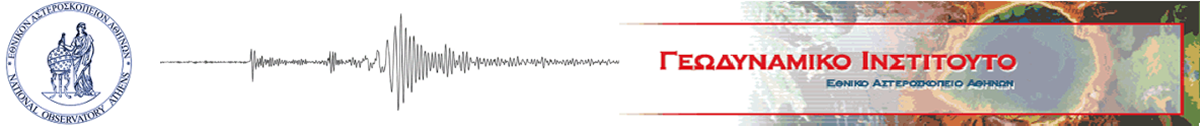
\includegraphics[height=2.5em]{../../logos/gein_logo.png} 
\includegraphics[height=2.5em]{../../logos/egu19_logo.png} 
\includegraphics[height=2.5em]{../../logos/epos_logo_big.jpg}} % Second university/lab logo on the right

 }
{
\includegraphics[height=6em]{../../logos/egu24_logo.png}} % 
\includegraphics[height=6.5em]{../../logos/logo_uoa_blue.png}} % Second university/lab logo on the right
%----------------------------------------------------------------------------------------
%	INTRODUCTION
%----------------------------------------------------------------------------------------

\headerbox{Introduction}{name=introduction,column=0,row=0}{
In this study we present preliminarily results of an ongoing research project between Dionysos Satellite Observatory (DSO) and the Hellenic Cadastre. The latter, has installed since 2007 a dense national network of 98 GPS/GNSS sites, spatially covering the whole country. Selected datasets of the network data were incorporated into the automatic processing infrastructure developed and maintained by DSO to perform an in-depth study and monitoring of the geodynamic and seismic setting of Hellenic region. Further collaboration and integration of both historic and contemporary data can signifficantly strengthen our understanding of the complicated geotectonic setting in one of the most actively tectonic regions of the world.

\begin{center}
\begin{tcolorbox}[height=2.5em,width=.7\textwidth,colback={airforceblue}, colupper=white,  boxrule=0pt]   
 \textbf{Abstract Number:  EGU2024-17390}
\end{tcolorbox}  
 \end{center}
% \vspace{0.3em} % When there are two boxes, some whitespace may need to be added if the one on the right has more content
}

%----------------------------------------------------------------------------------------
%	VELOCITY FIELD
%----------------------------------------------------------------------------------------

\headerbox{Estimation of Velocity Field}{name=data,column=2, span=2,row=0}{
% \vfill
\begin{minipage}[c]{0.31\linewidth}
Following the estimation of daily site coordinates, position time-series were stacked for every site of the network. The latter wre in turn analyzed using the Hector software (Bos et al., 2013) for the estimation of tectonic velocities and harmonic signals. The time span of more than ten years allows estimation of site velocities, yet the temporal density of data could inhibit the accuracy that can be obtained.

%  The daily position estimates of the stations are automatically logged into suitable files, from which position time series are generated. Time series analysis use to estimate coordinates (within a specified Reference Frame IGb14), tectonic velocities, harmonic signals, co-seismic displacements and volocity changes. The analysis was conducted using the Free Software/Open Source Software Hector (Bos, 2013), with requisite adjustments made as necessary.
\end{minipage}
\begin{minipage}[c]{0.02\linewidth}

\end{minipage}
\begin{minipage}[c]{0.33\linewidth}
   Time series analysis of three different station are presented.
   Velocity field with respect to IGb14 presented on the following map.\\[.4em]
  Velocities vary per component:
  \begin{center}
  \vskip-.3cm
  \begin{tabular}{ c  c  c }
    \hline
      comp & min (mm/yr) & max (mm/yr)\\
    \hline
        North & -17.9 & 15.5 \\
        East & 2.4 & 26.0\\
        Up & -5.5 & 4.7 \\
    \hline
  \end{tabular}
  \end{center}

%  
%  North Greece WNW dir

%  Central GR Aegrean SW
    
\end{minipage}
\begin{minipage}[c]{0.34\linewidth}
  \begin{center}
  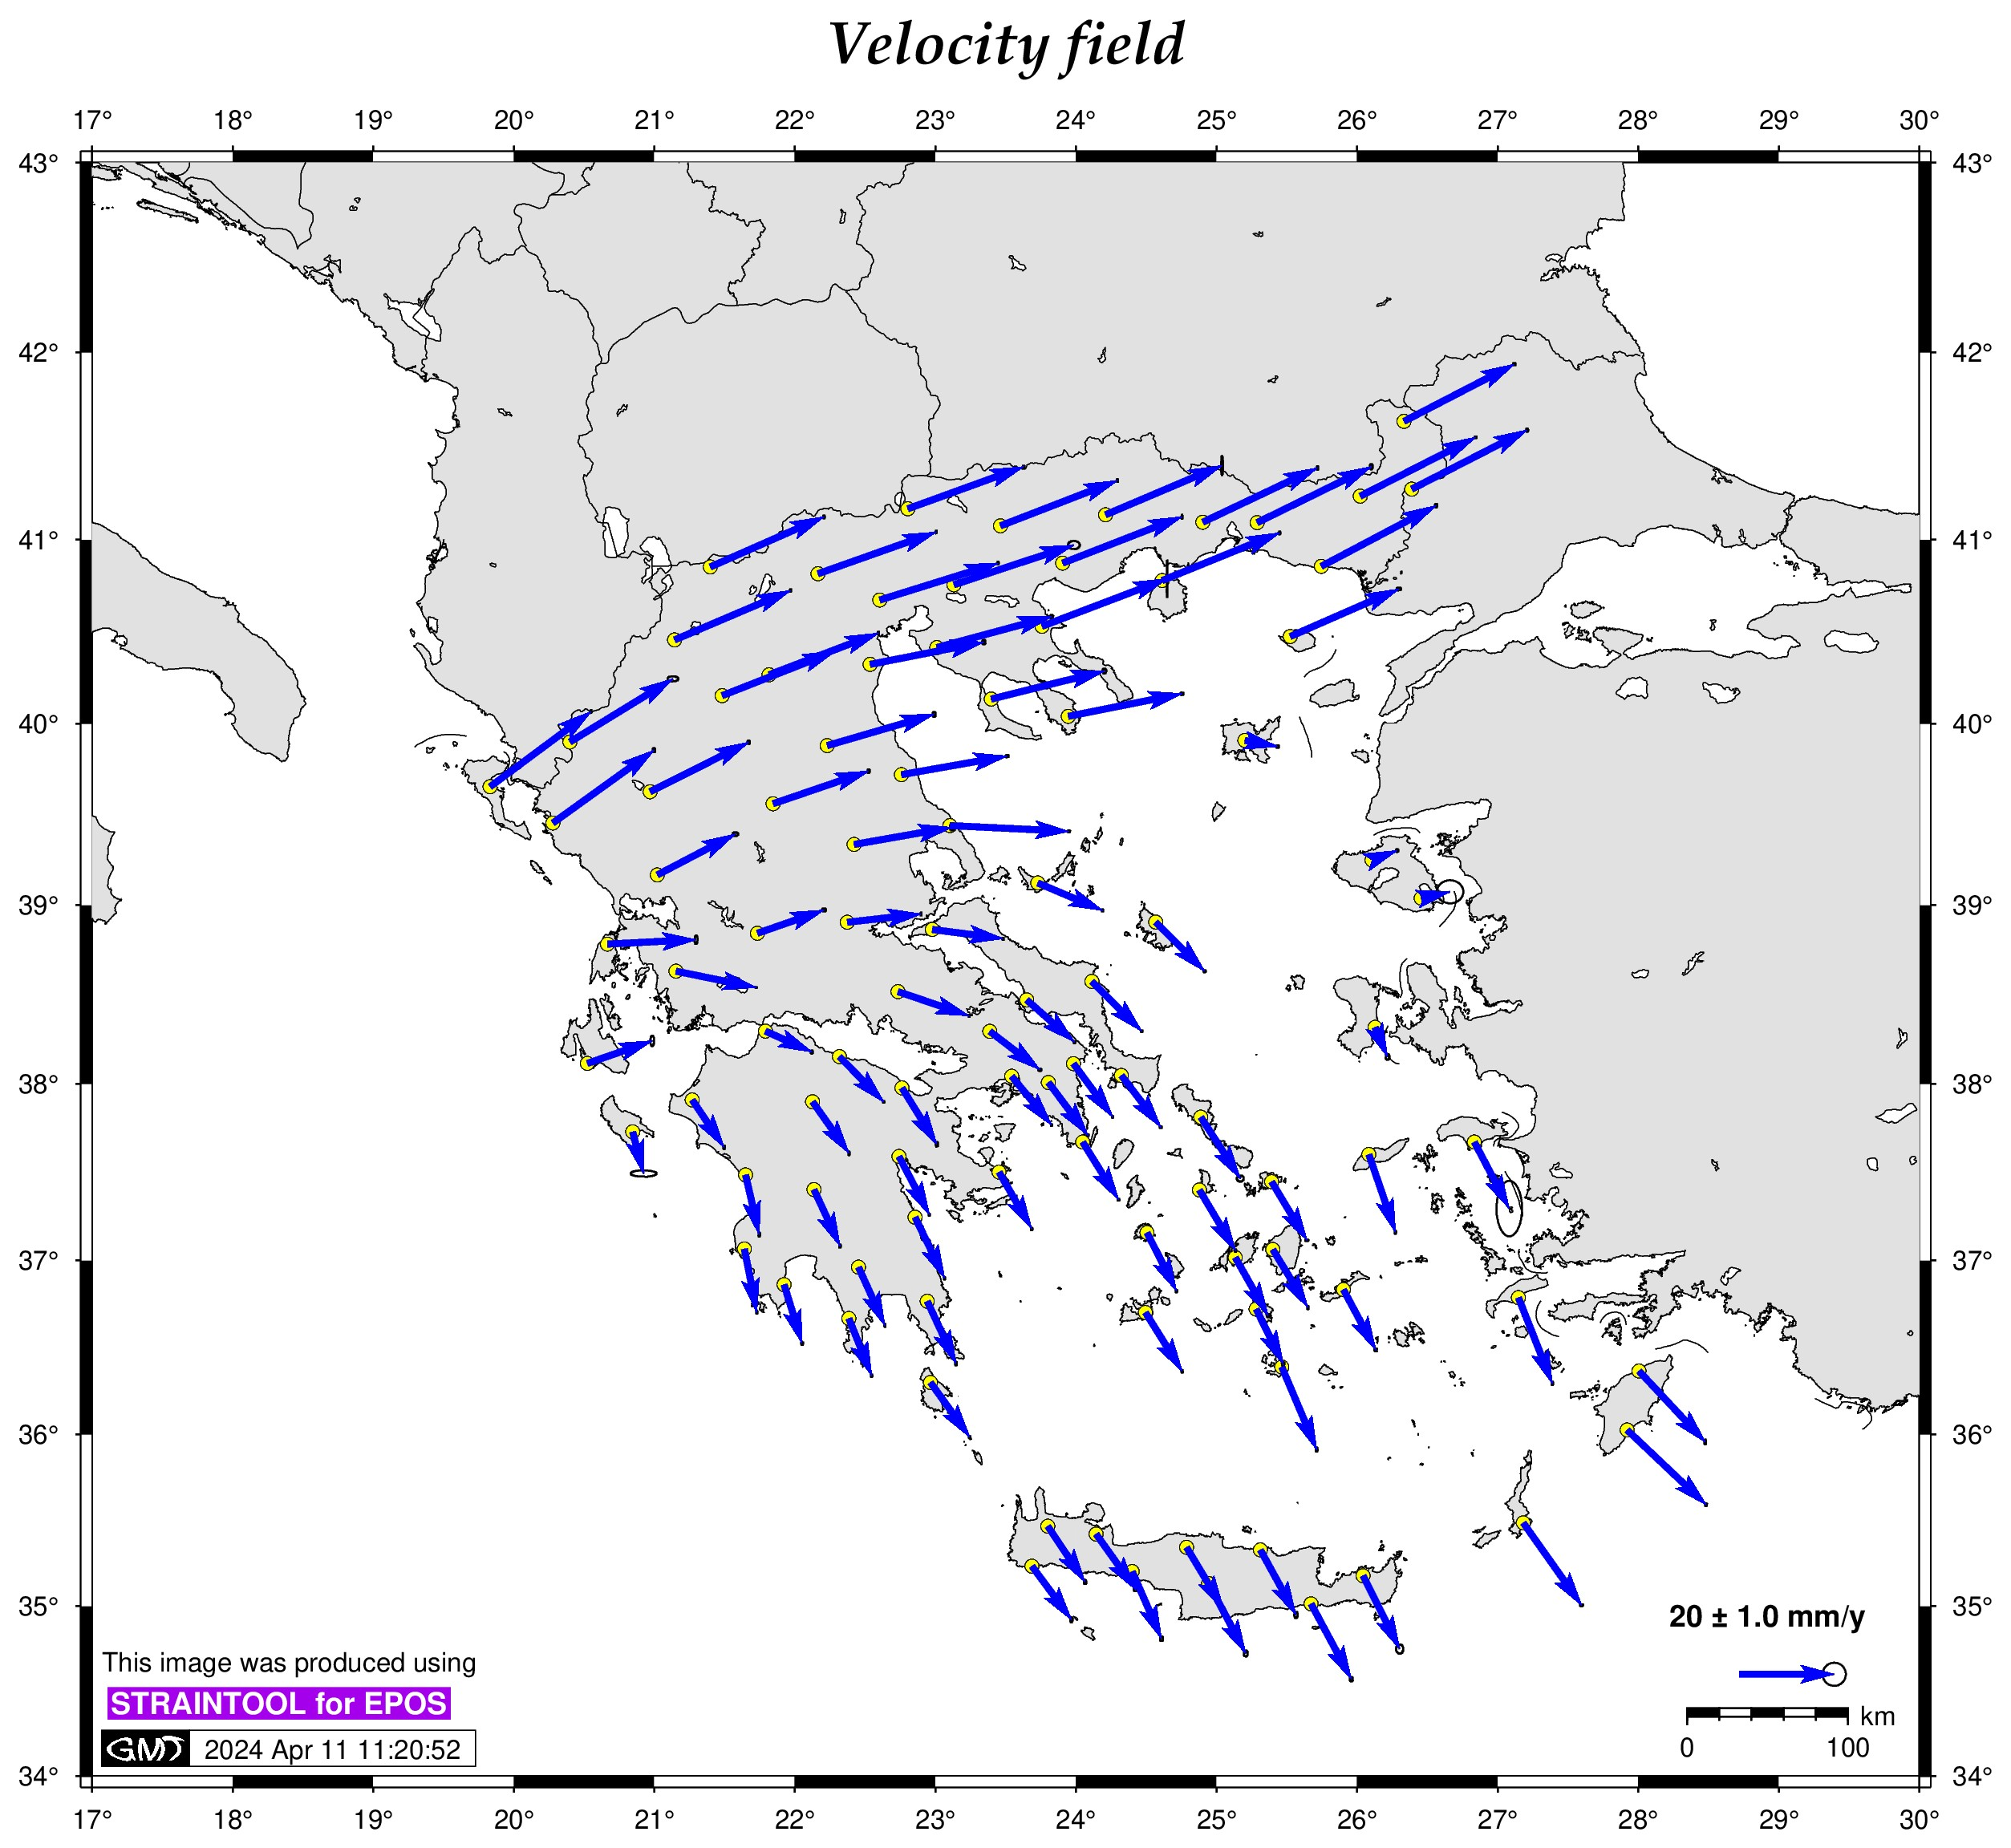
\includegraphics[width=.9\textwidth]{hepos22-output_vel.jpg}
  \end{center}
\end{minipage}

\begin{minipage}[c]{0.34\linewidth}
\begin{center}
098A
\end{center}
%\vfill
\rotatebox{90}{\scriptsize ~~~~~~~~~~North}
  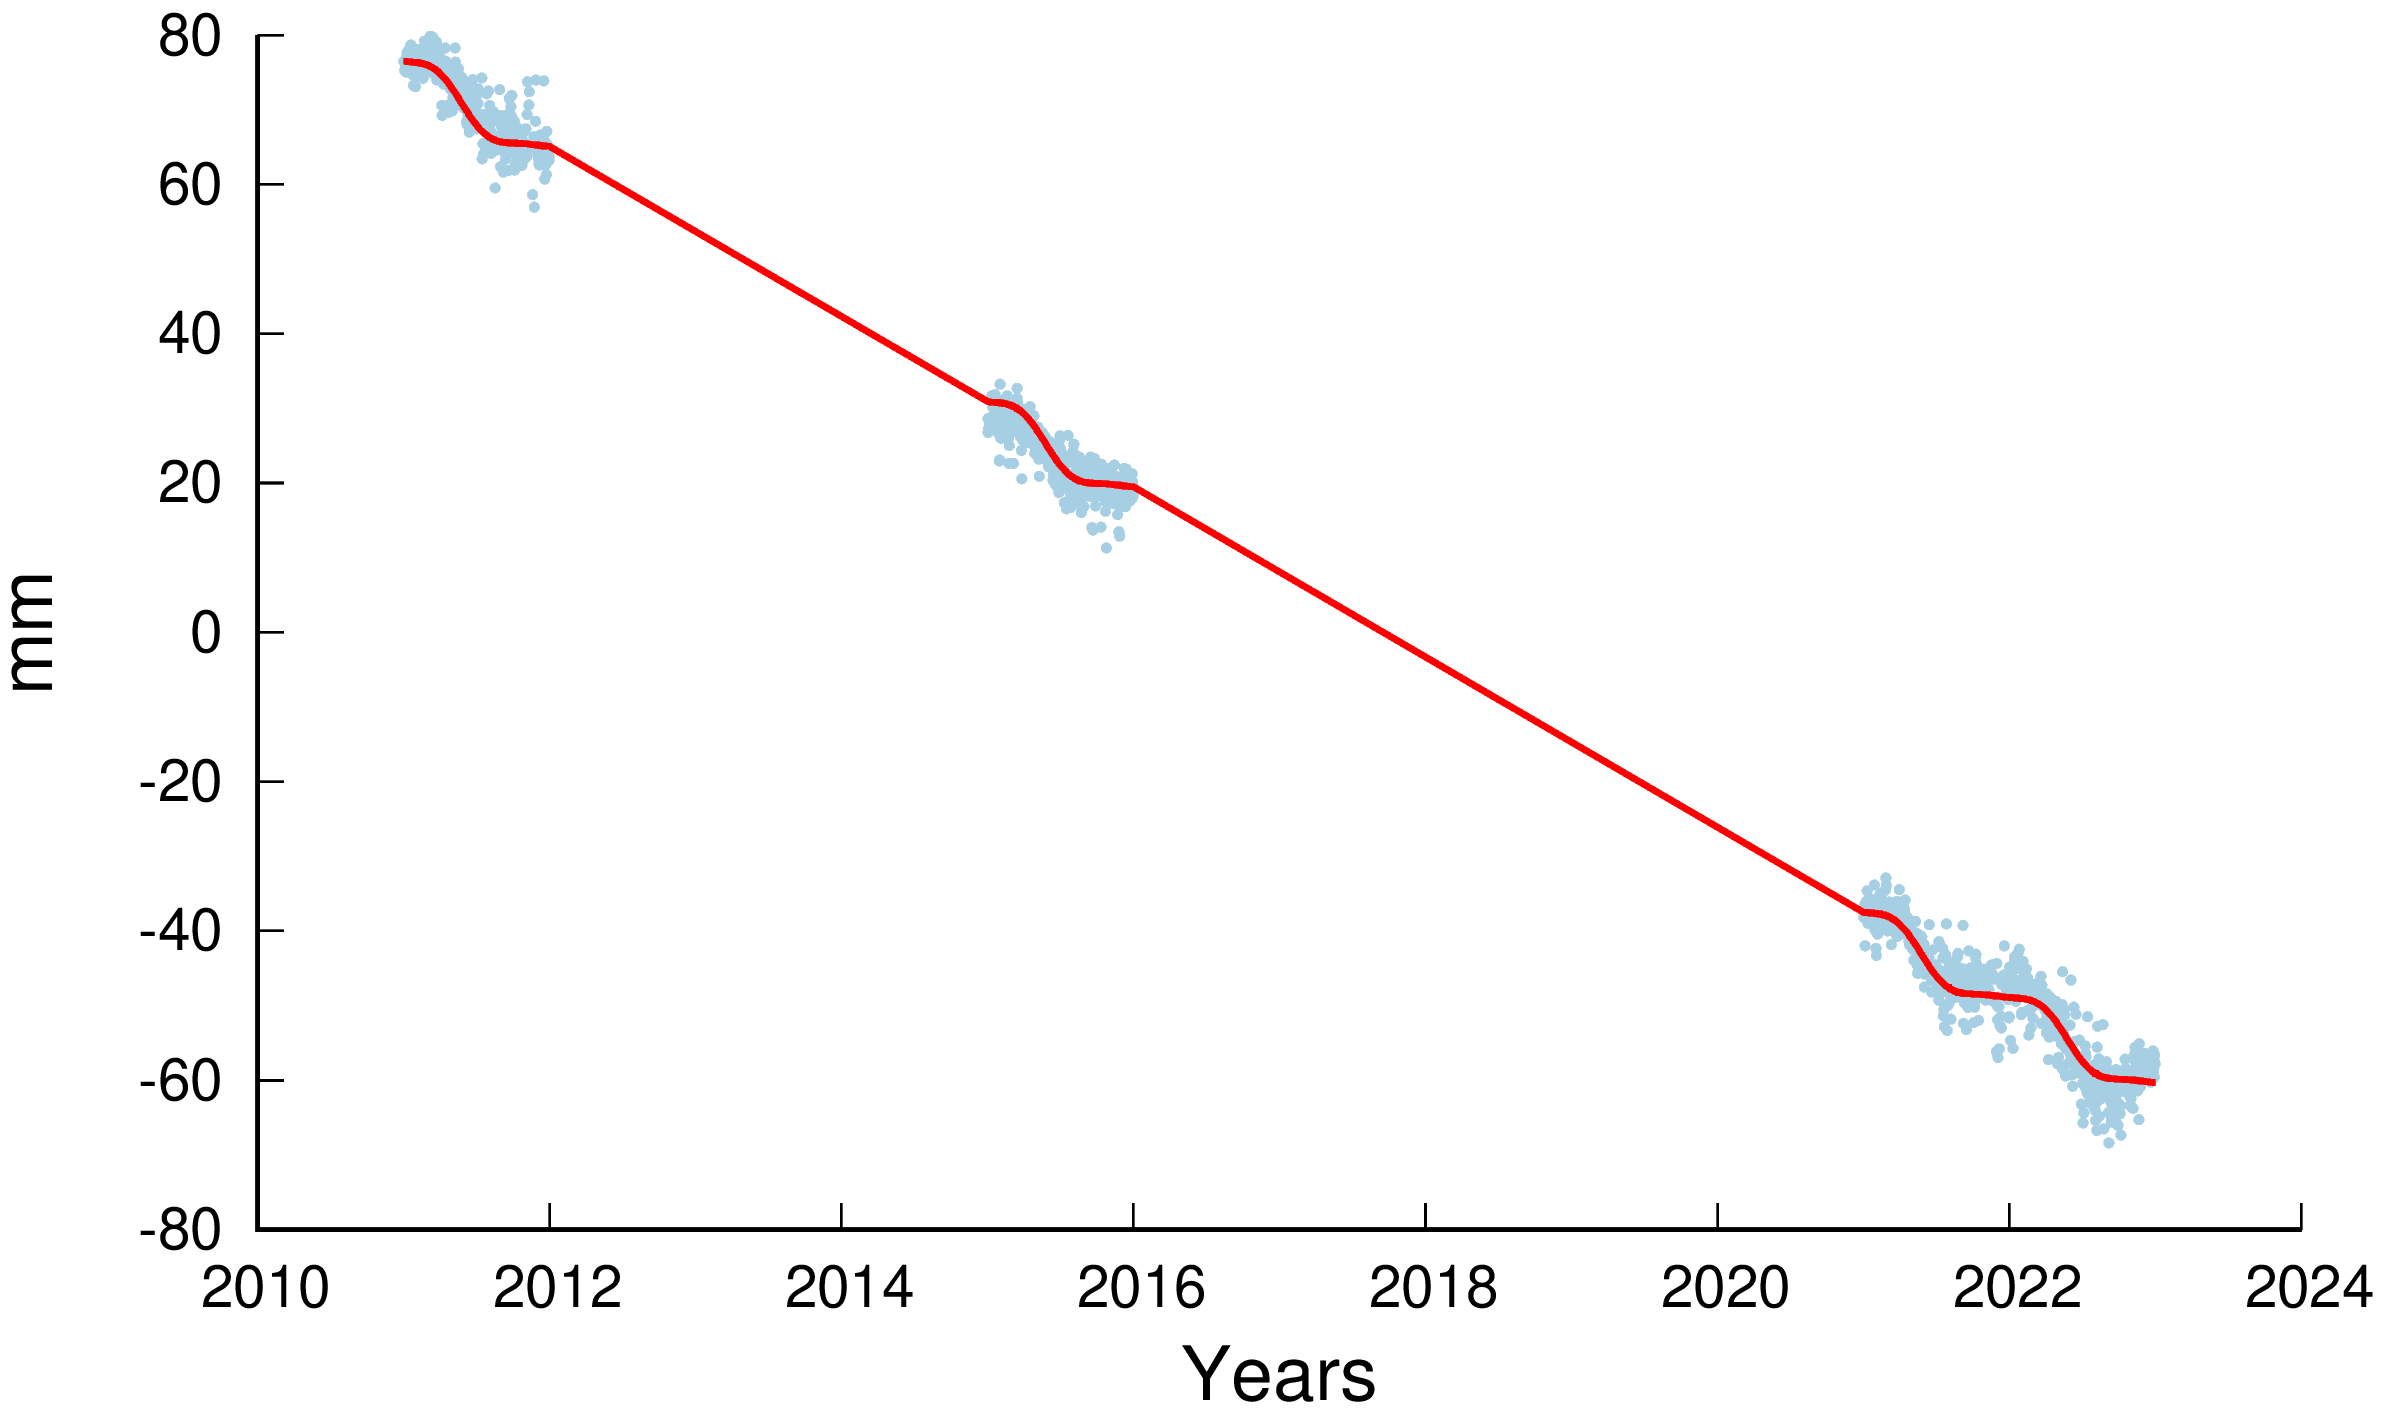
\includegraphics[height=5em]{098a_0_data.png}~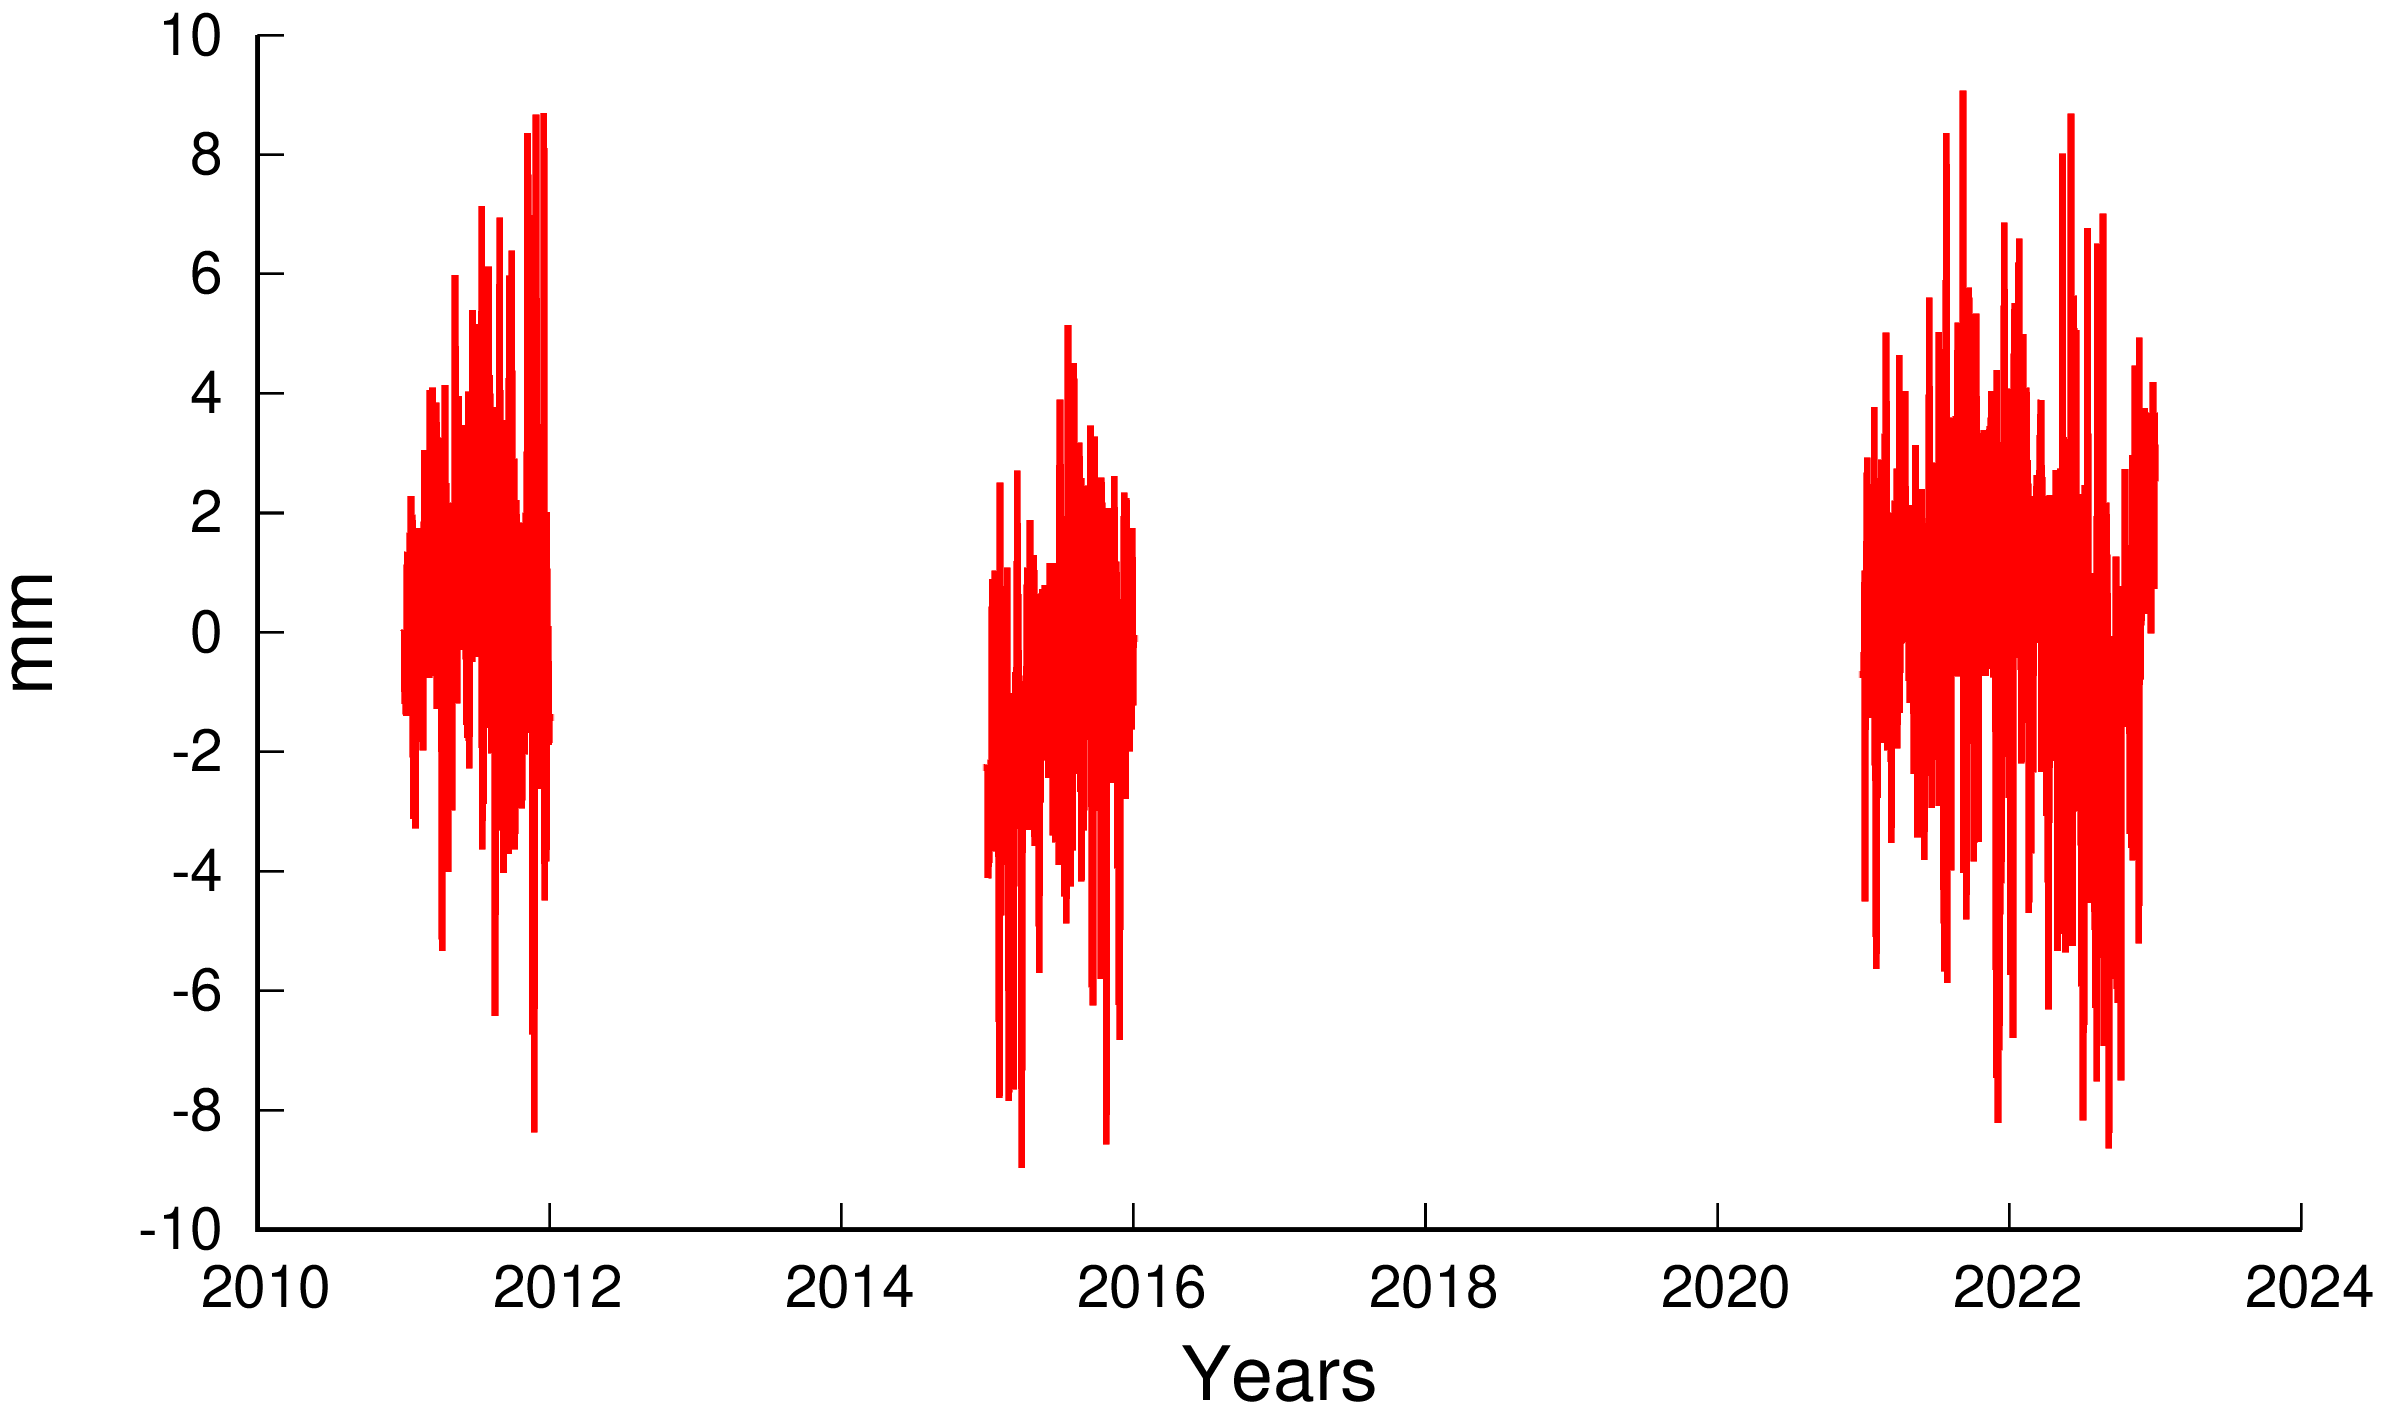
\includegraphics[height=5em]{098a_0_res.png}\\
\rotatebox{90}{\scriptsize ~~~~~~~~~~~~East}
  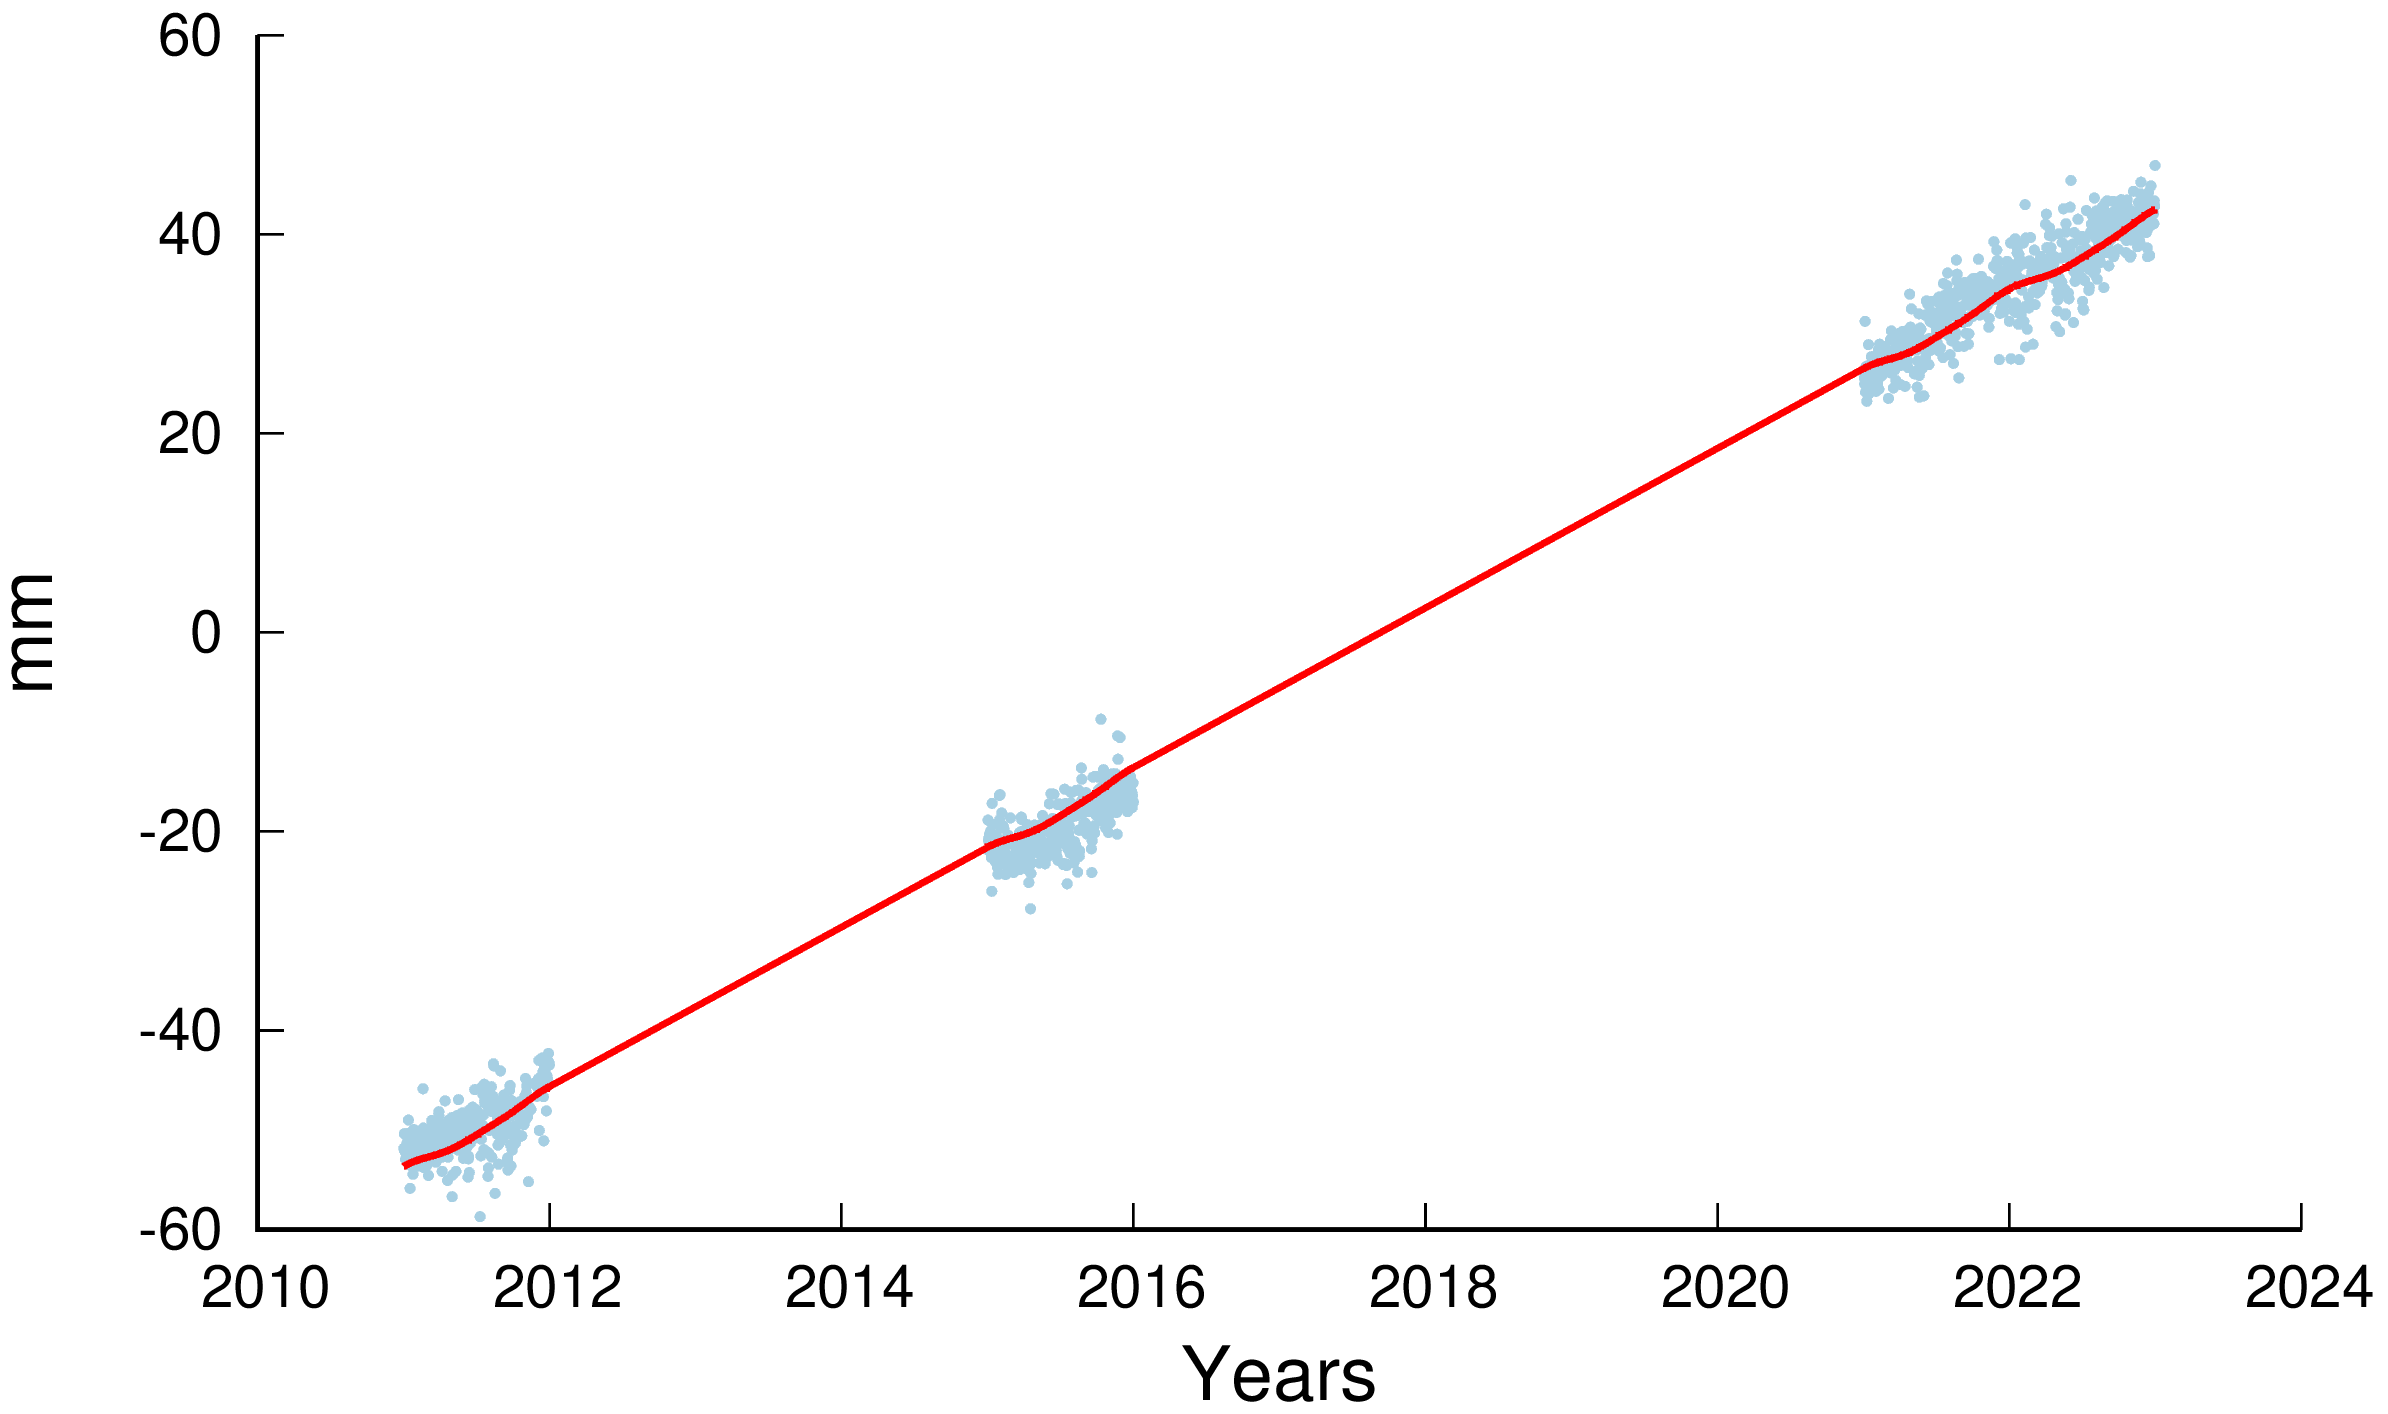
\includegraphics[height=5em]{098a_1_data.png}~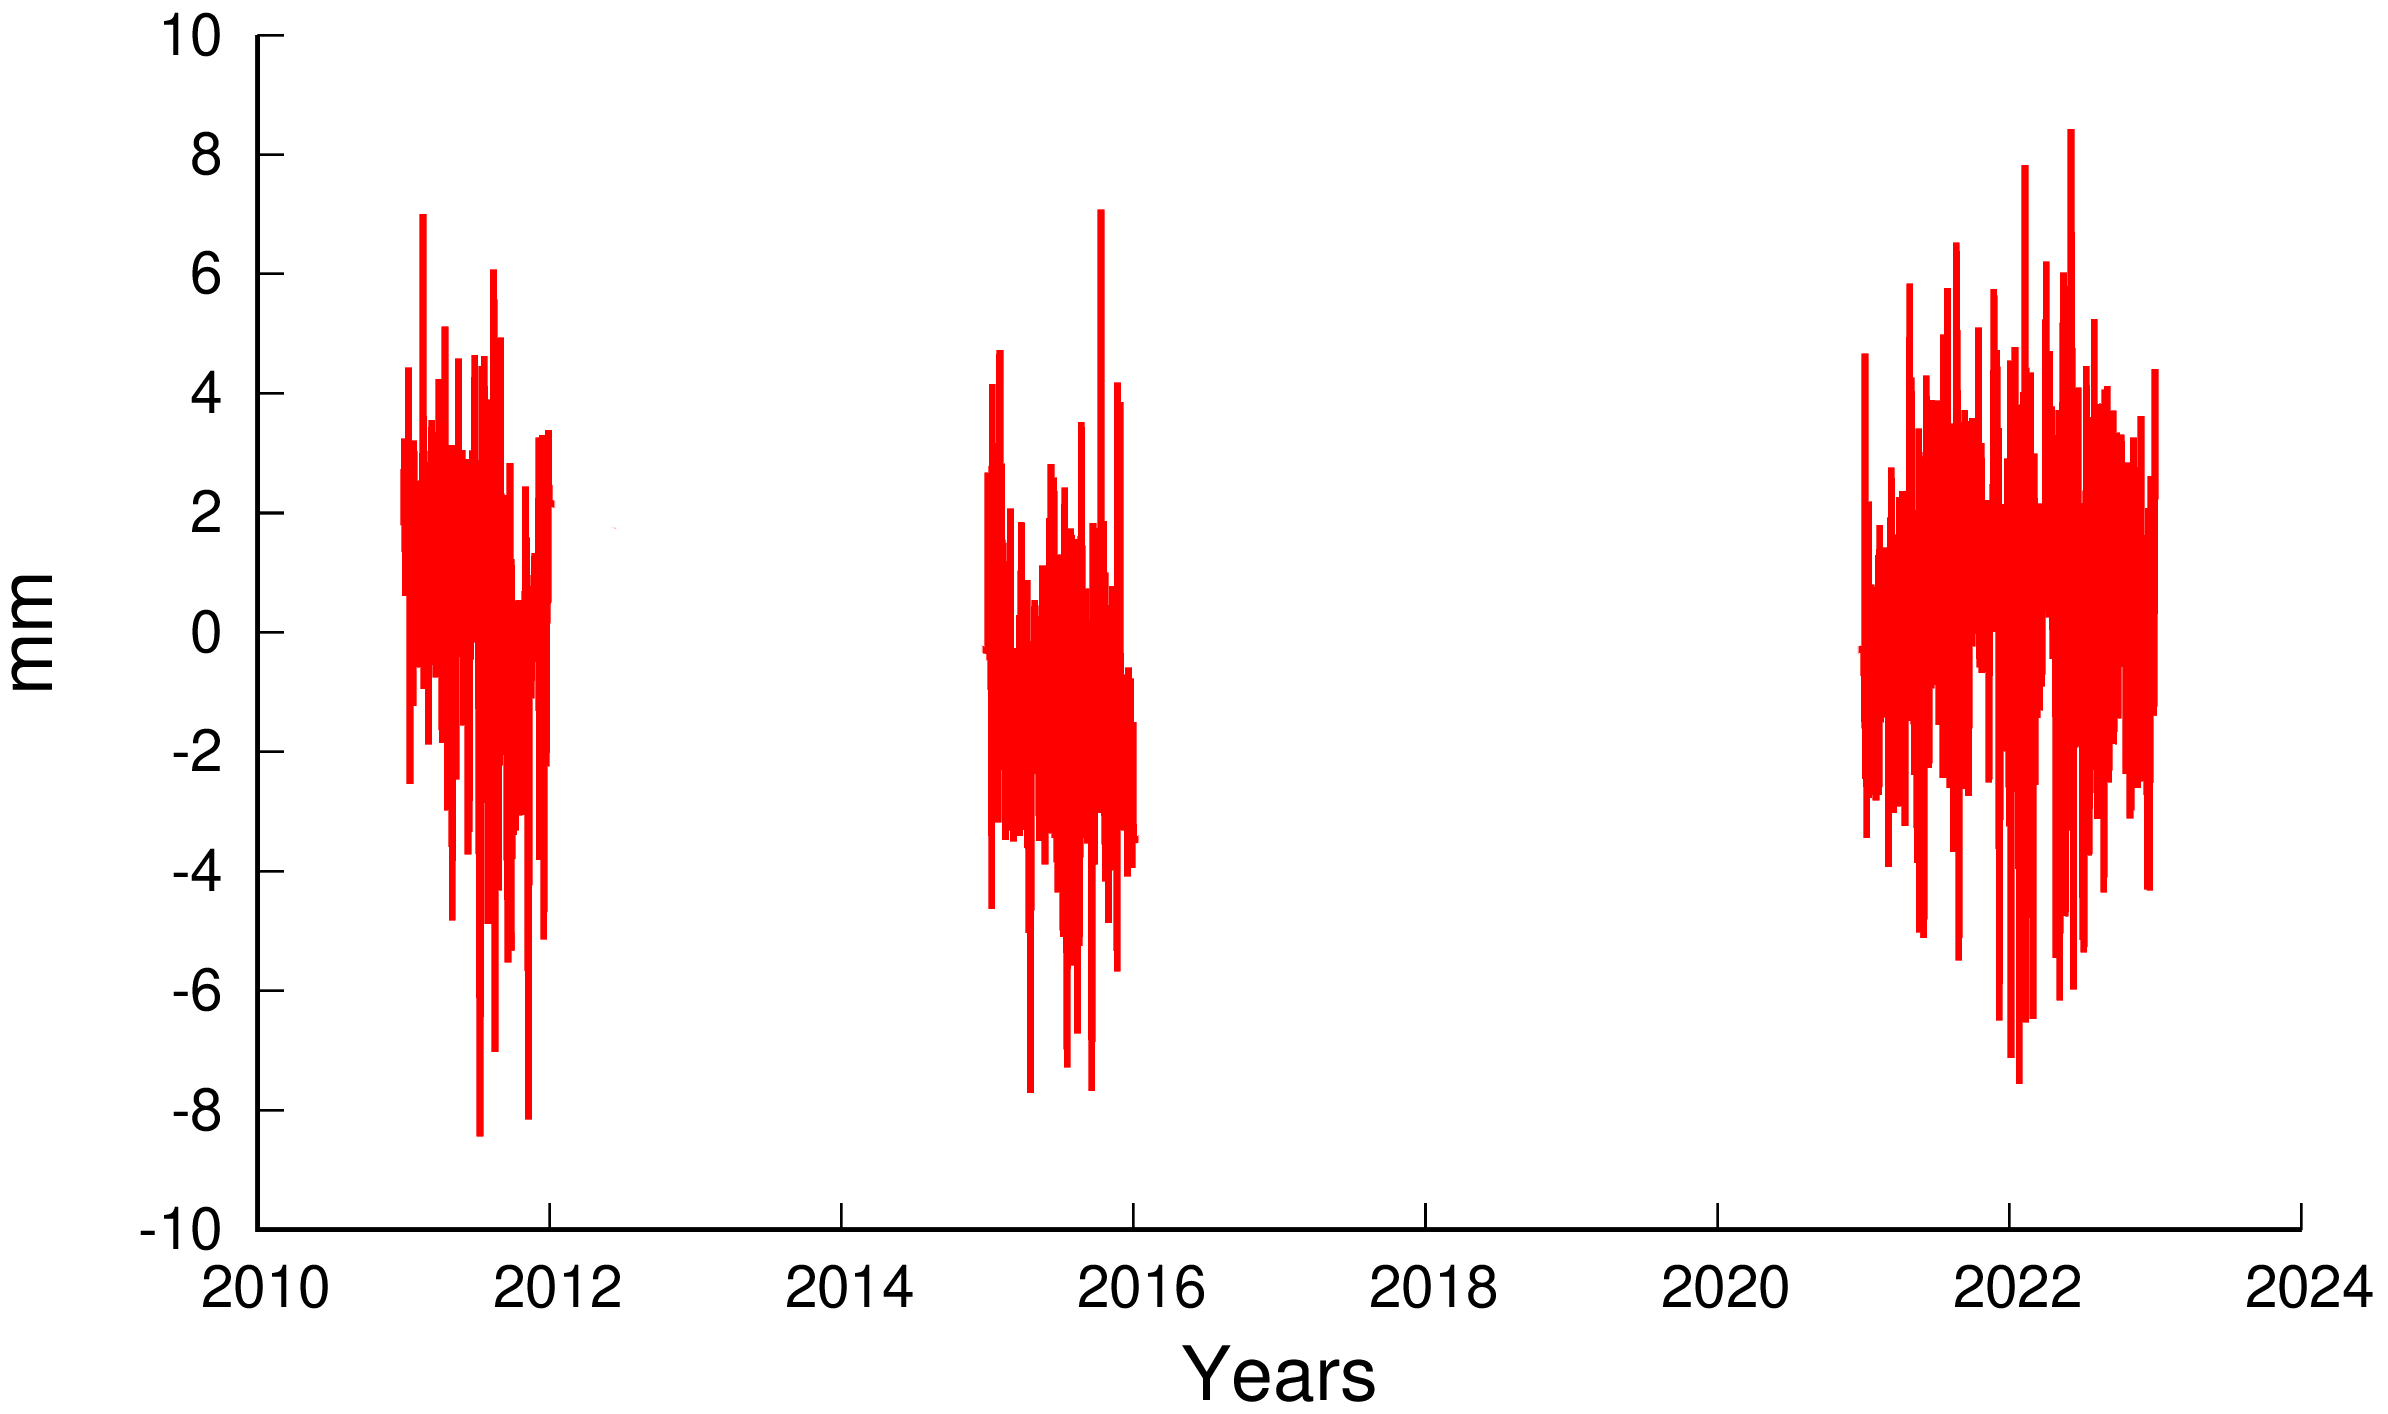
\includegraphics[height=5em]{098a_1_res.png}\\
\rotatebox{90}{\scriptsize ~~~~~~~~~~~~~~Up}
  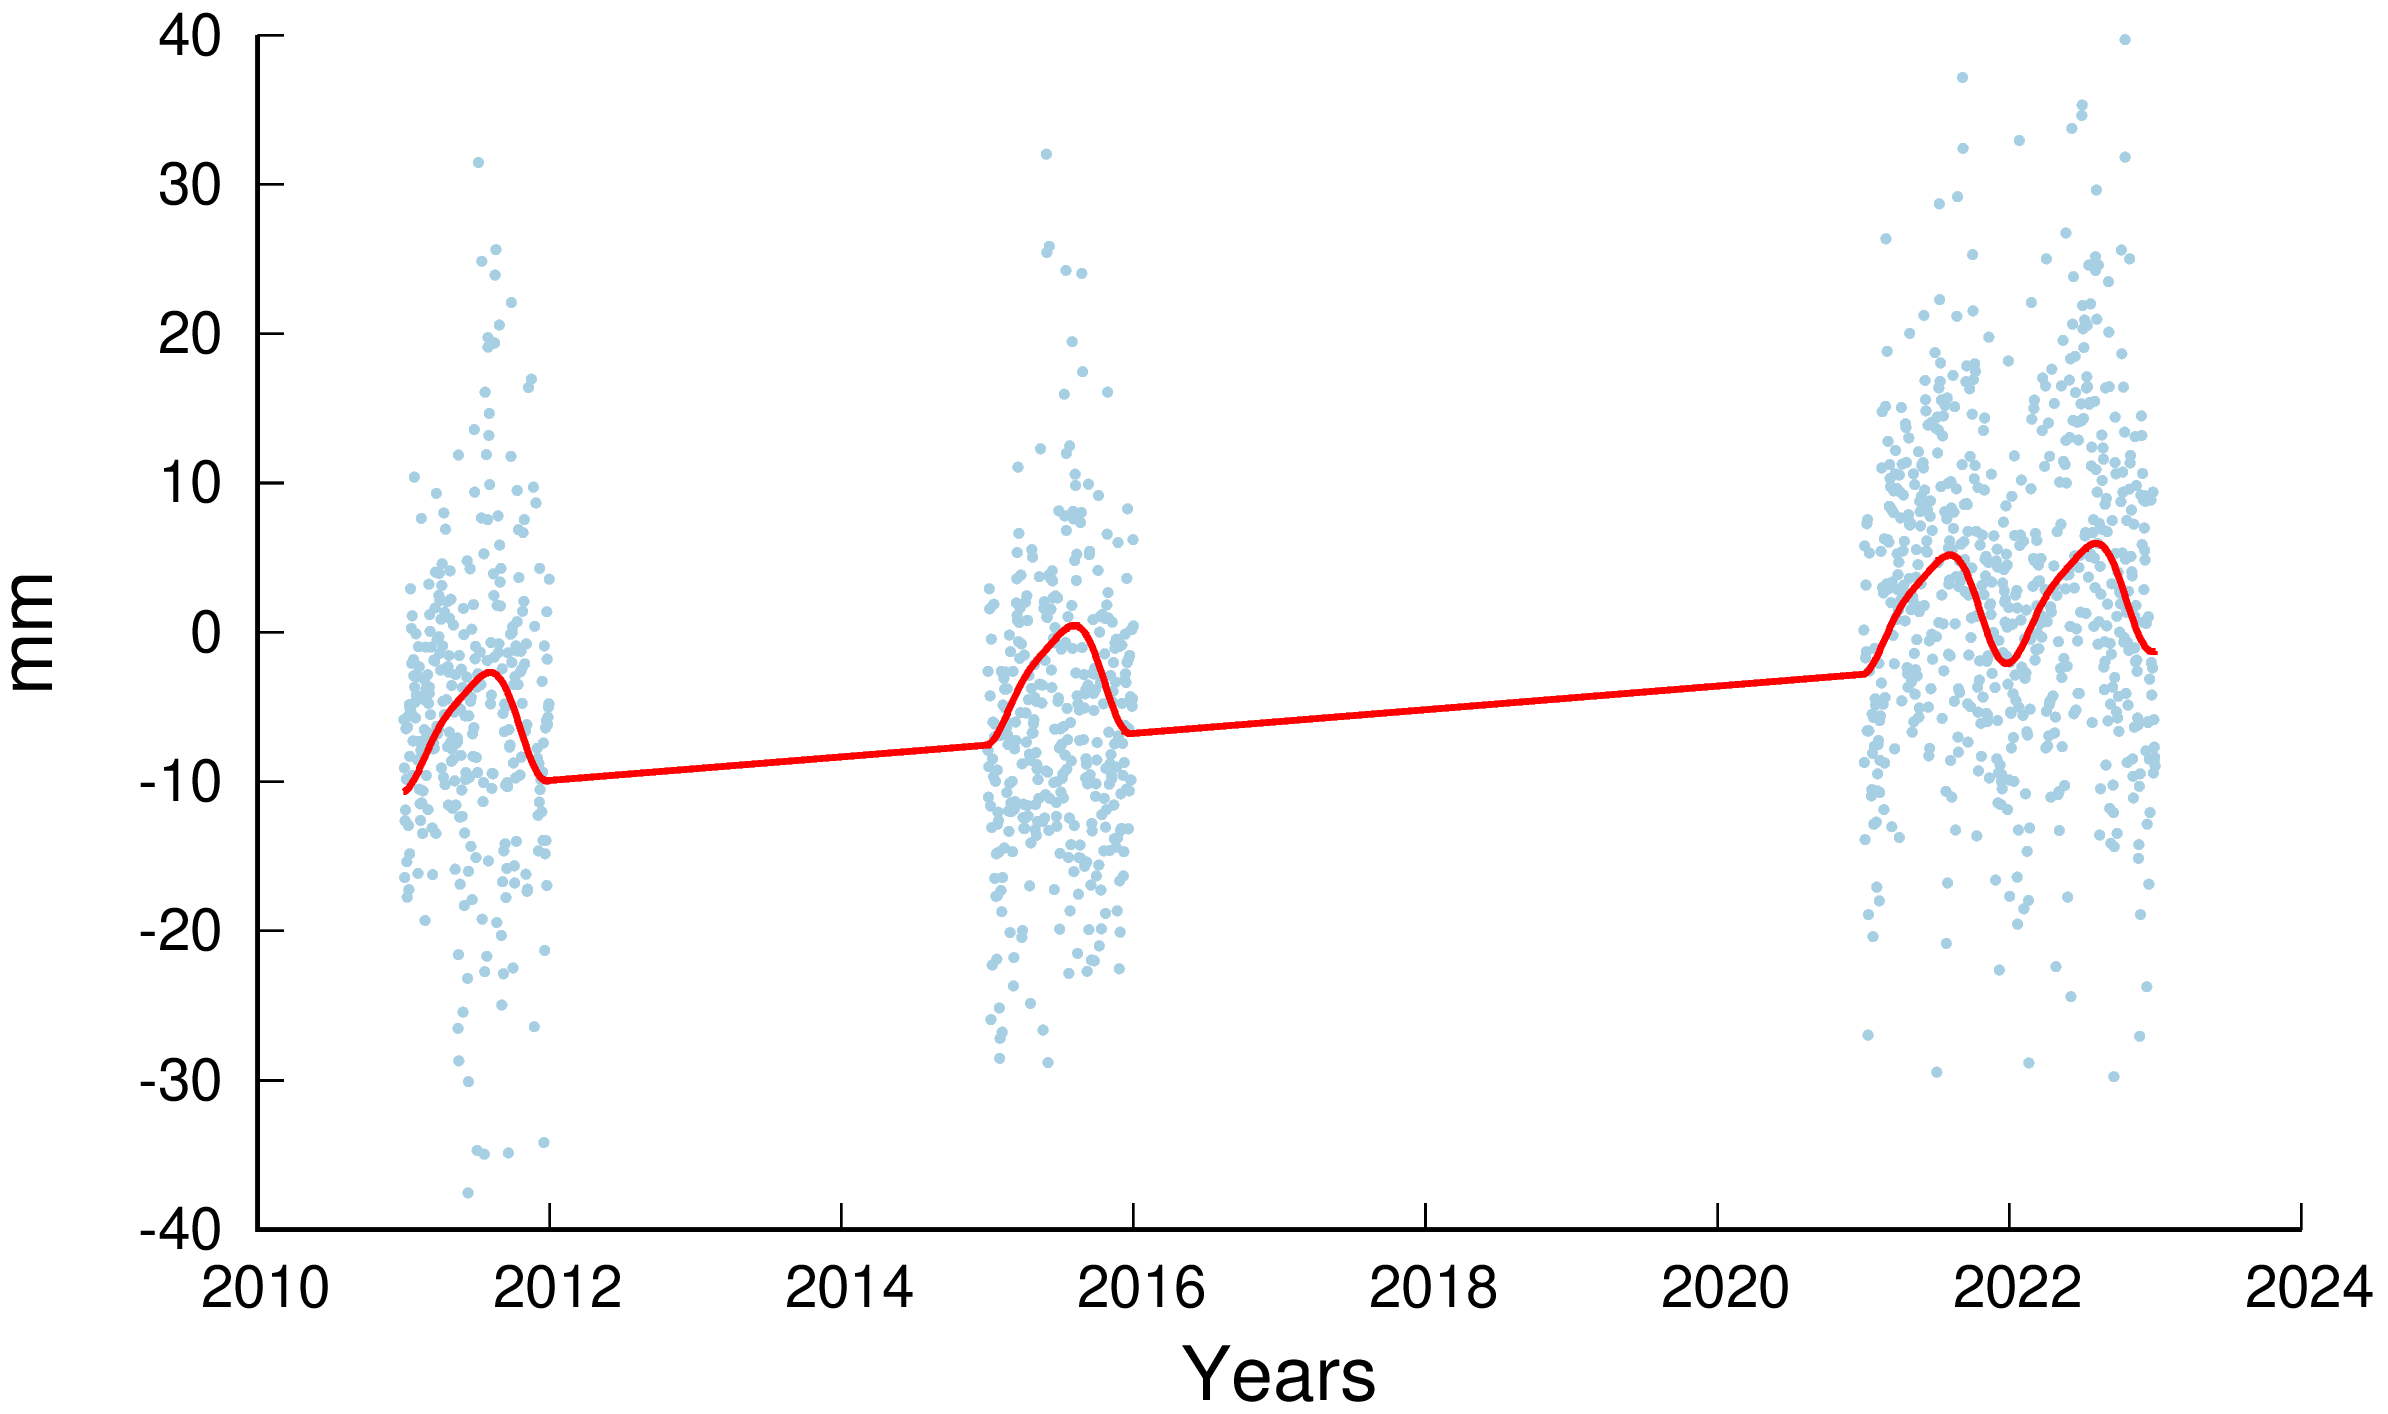
\includegraphics[height=5em]{098a_2_data.png}~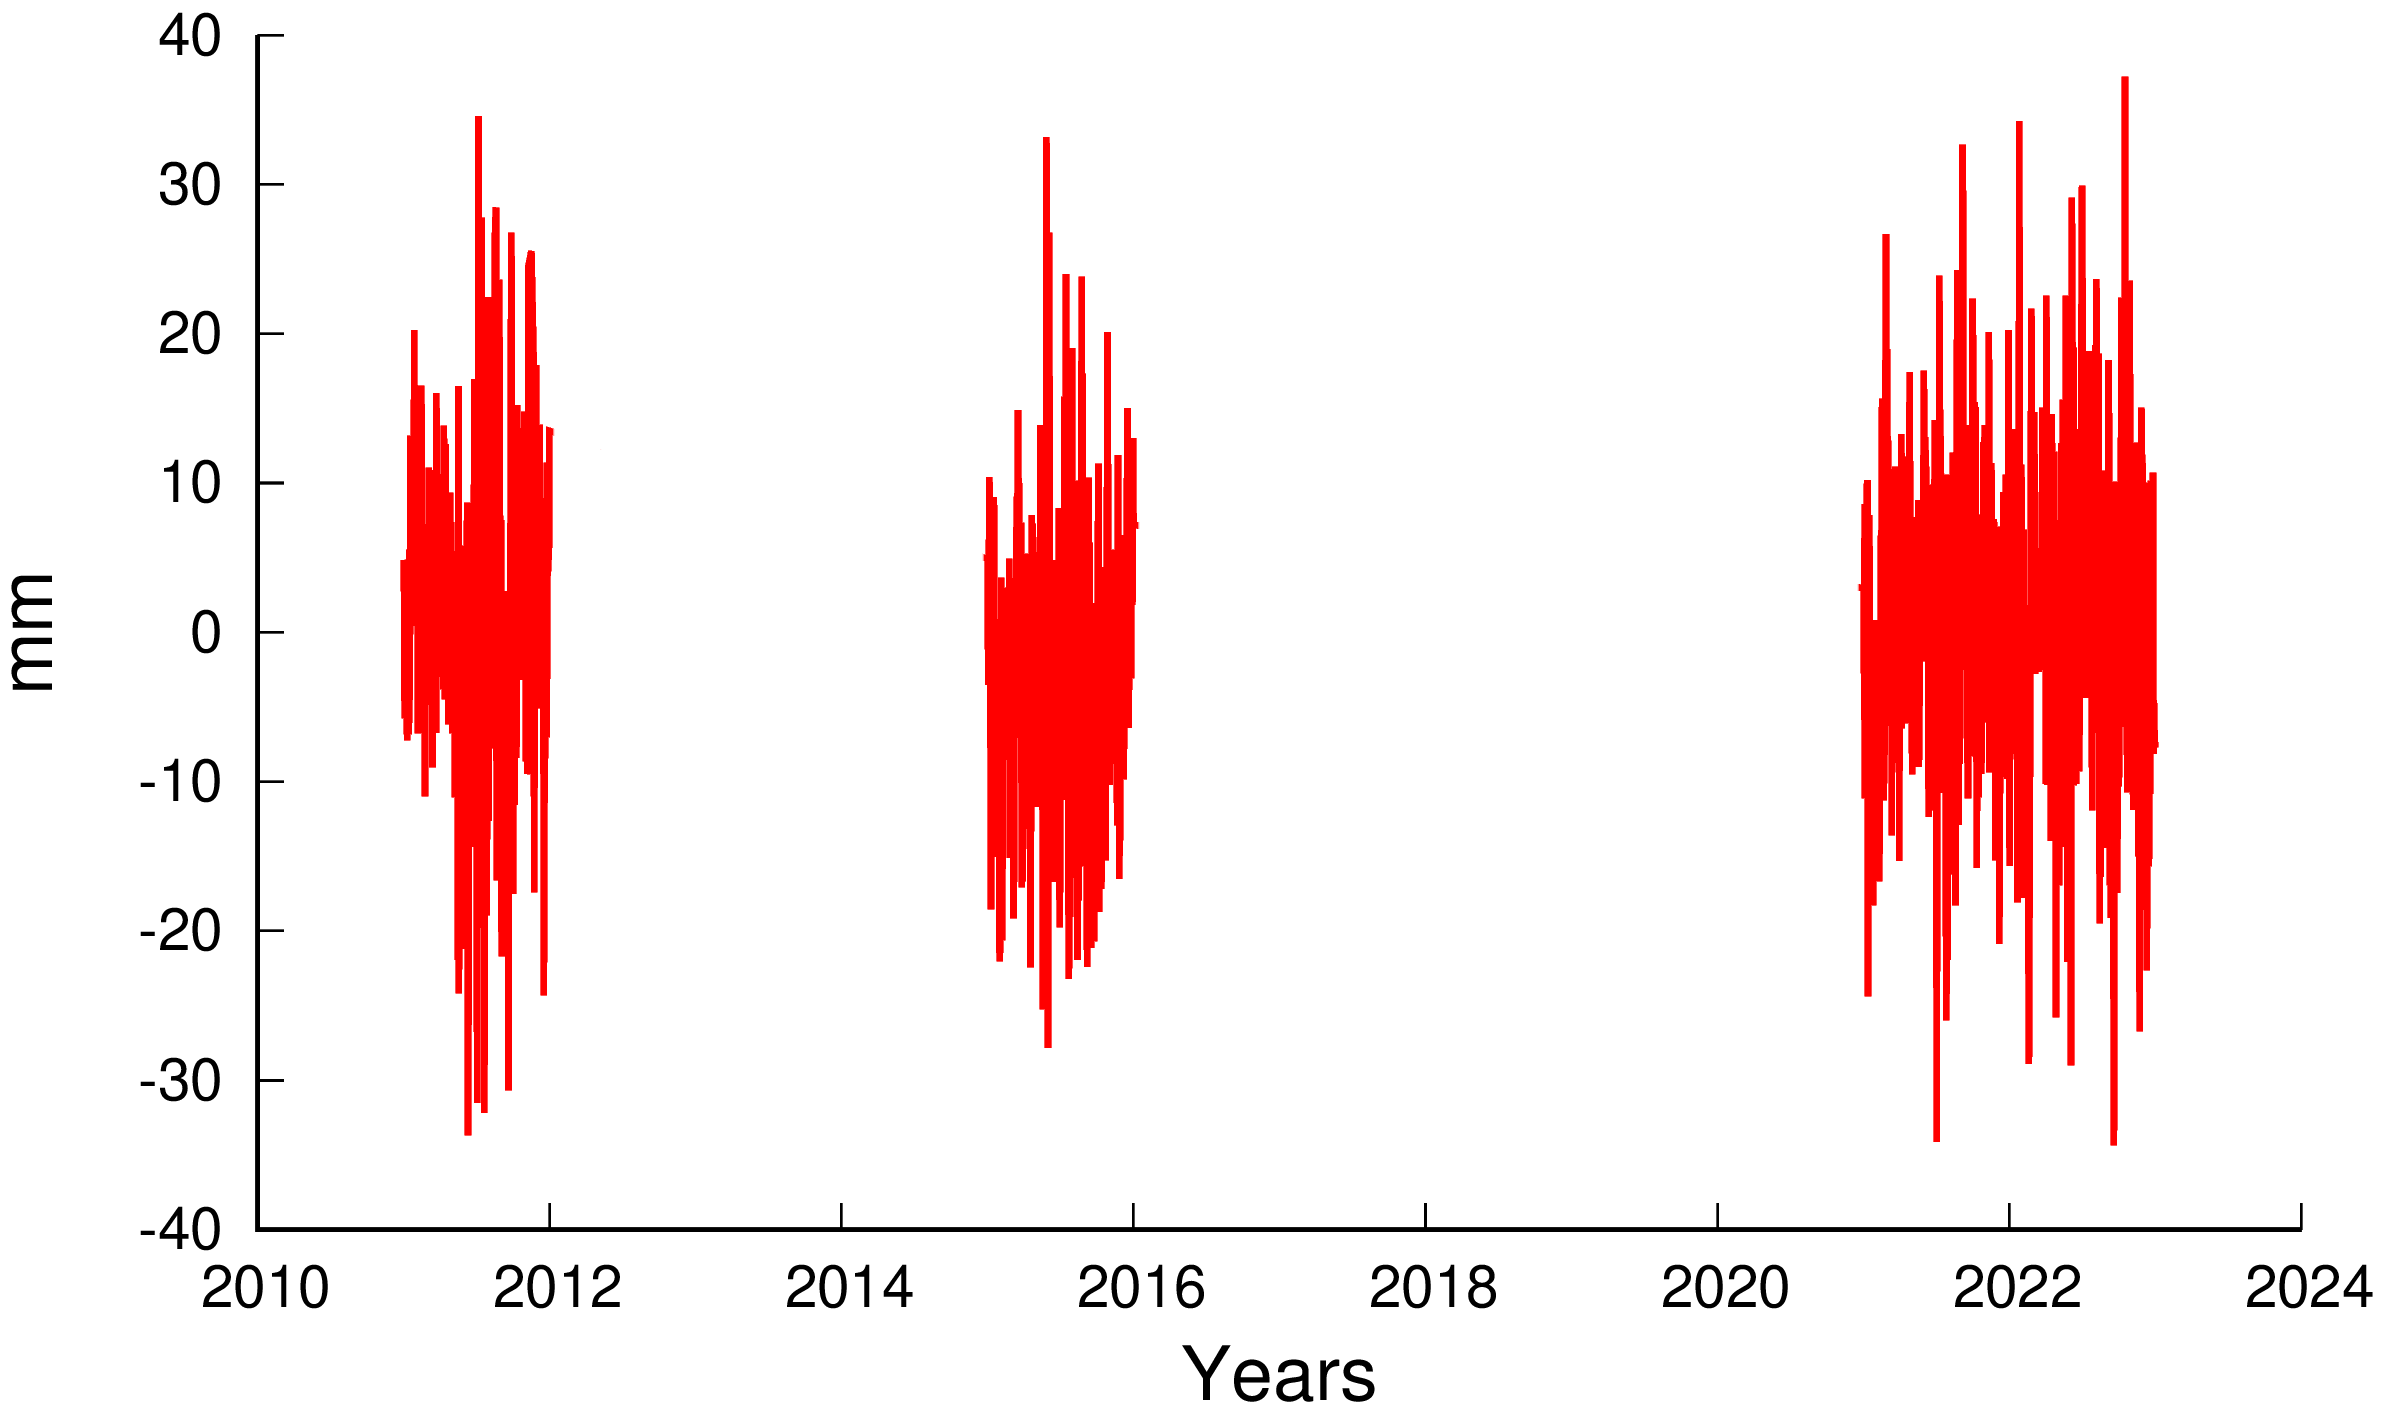
\includegraphics[height=5em]{098a_2_res.png}
%\vfill
\end{minipage}
\begin{minipage}[c]{0.33\linewidth}
\begin{center}
057A (co-seismic displacement)
\end{center}
  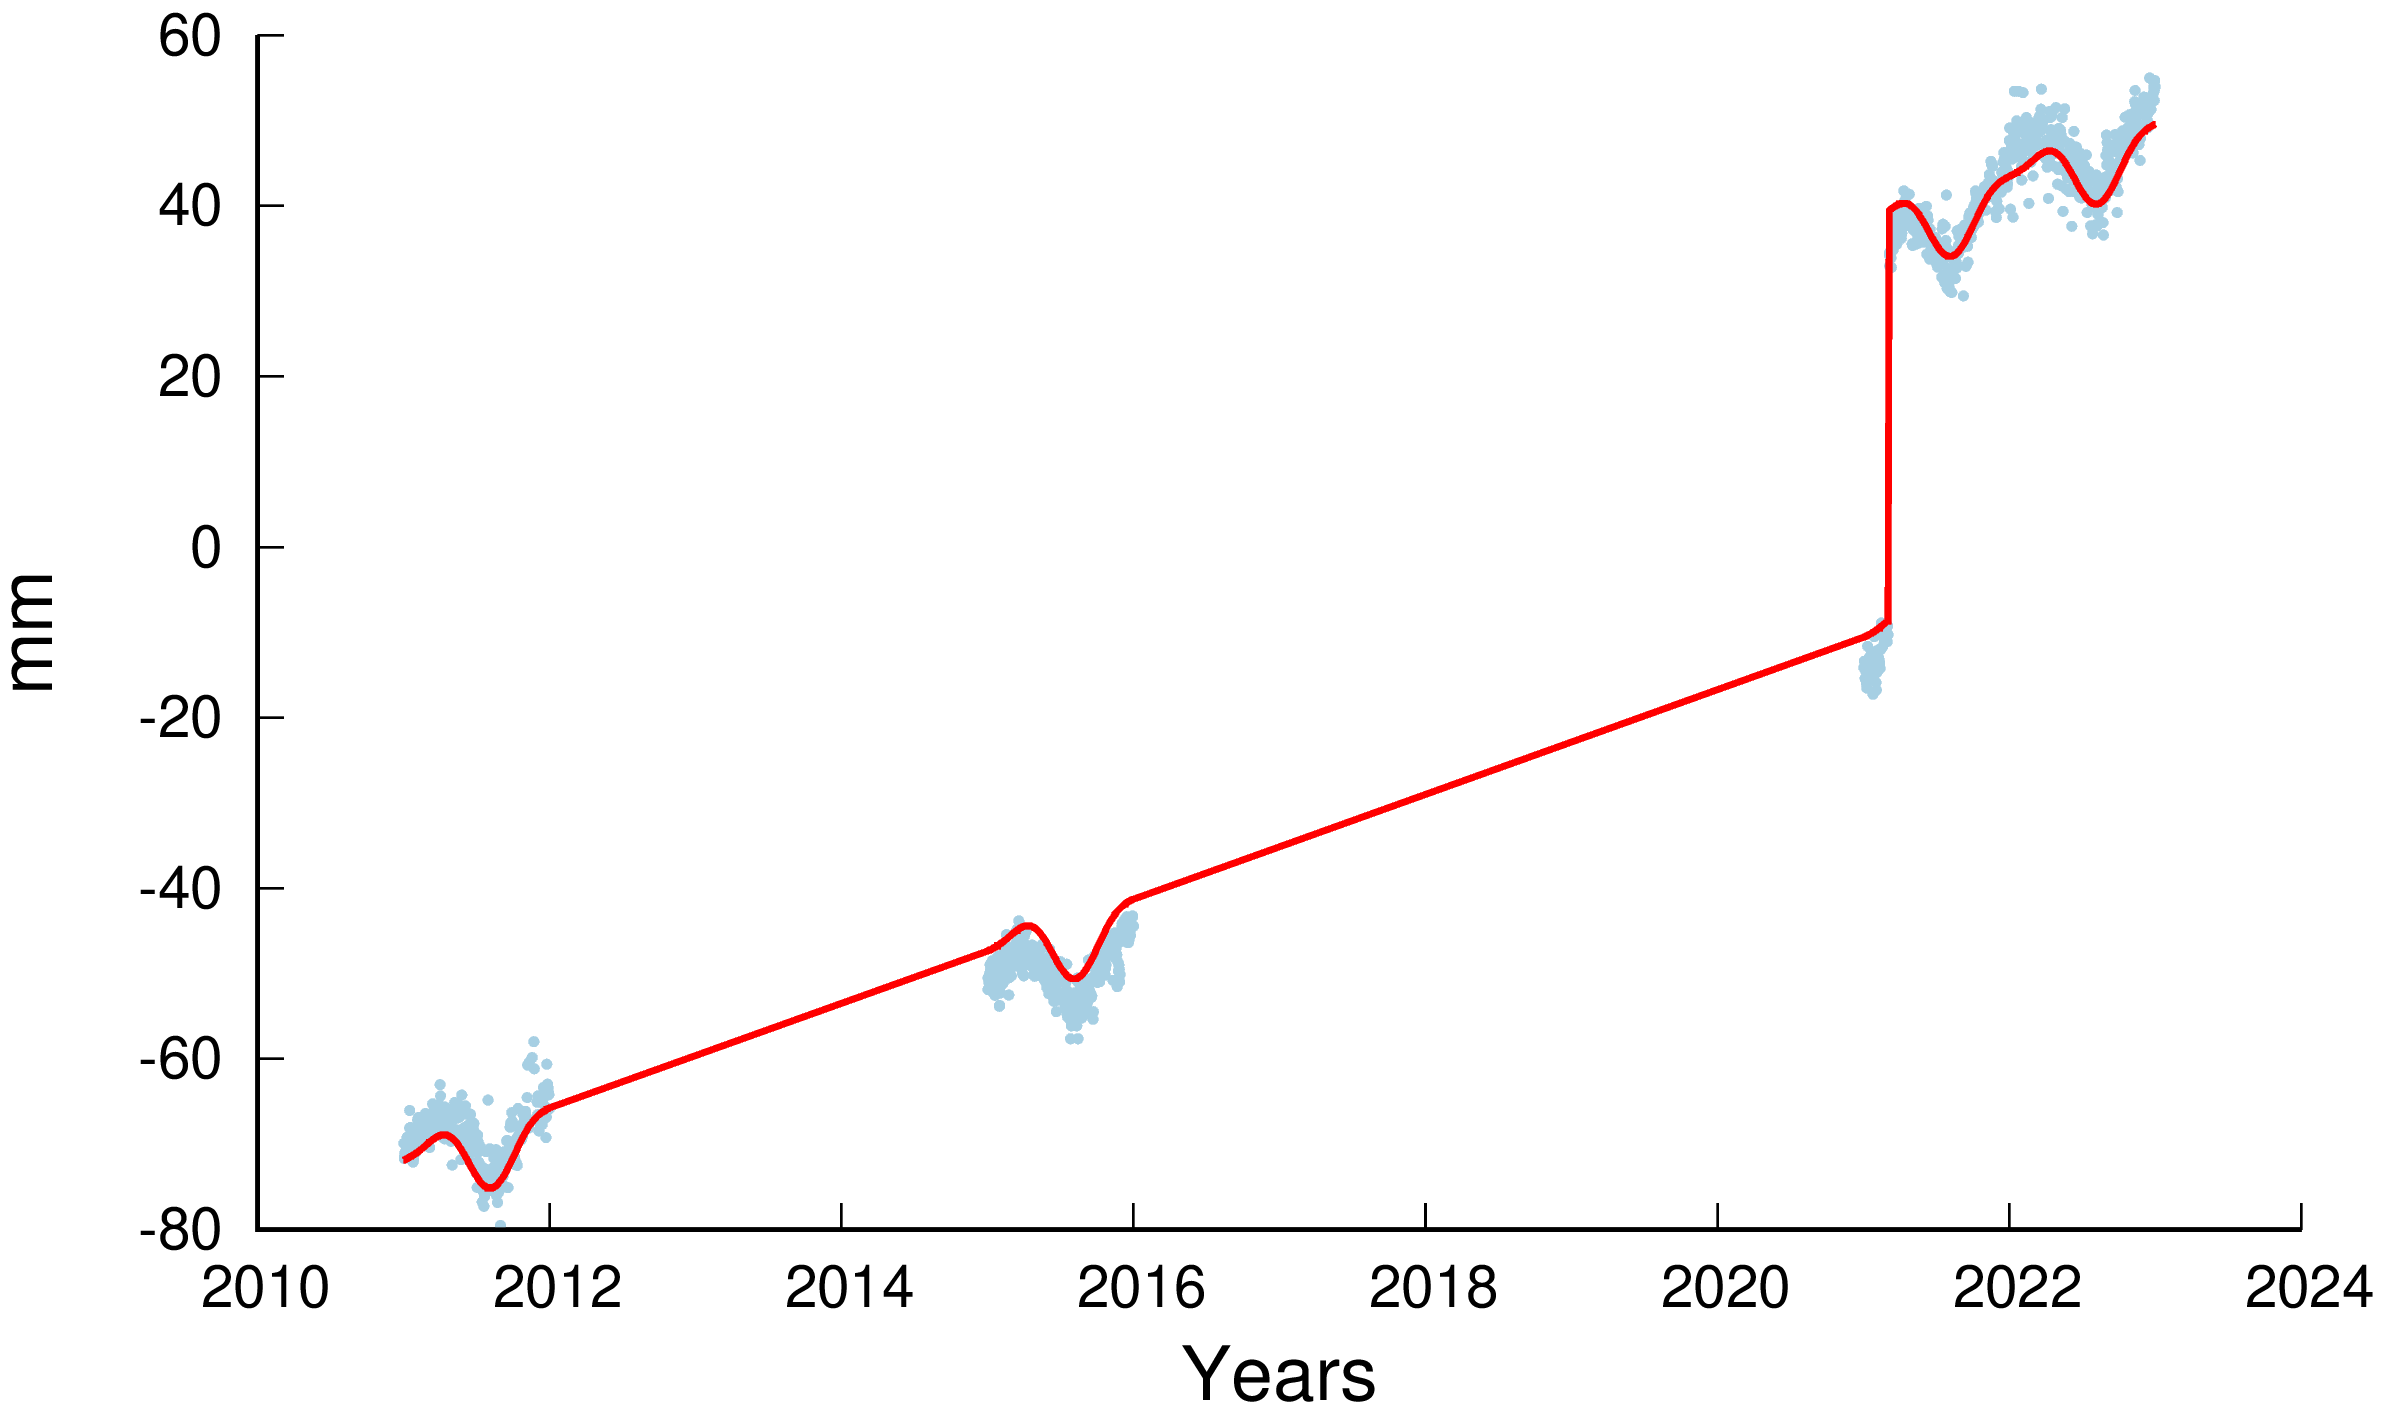
\includegraphics[height=5em]{057a_0_data.png}~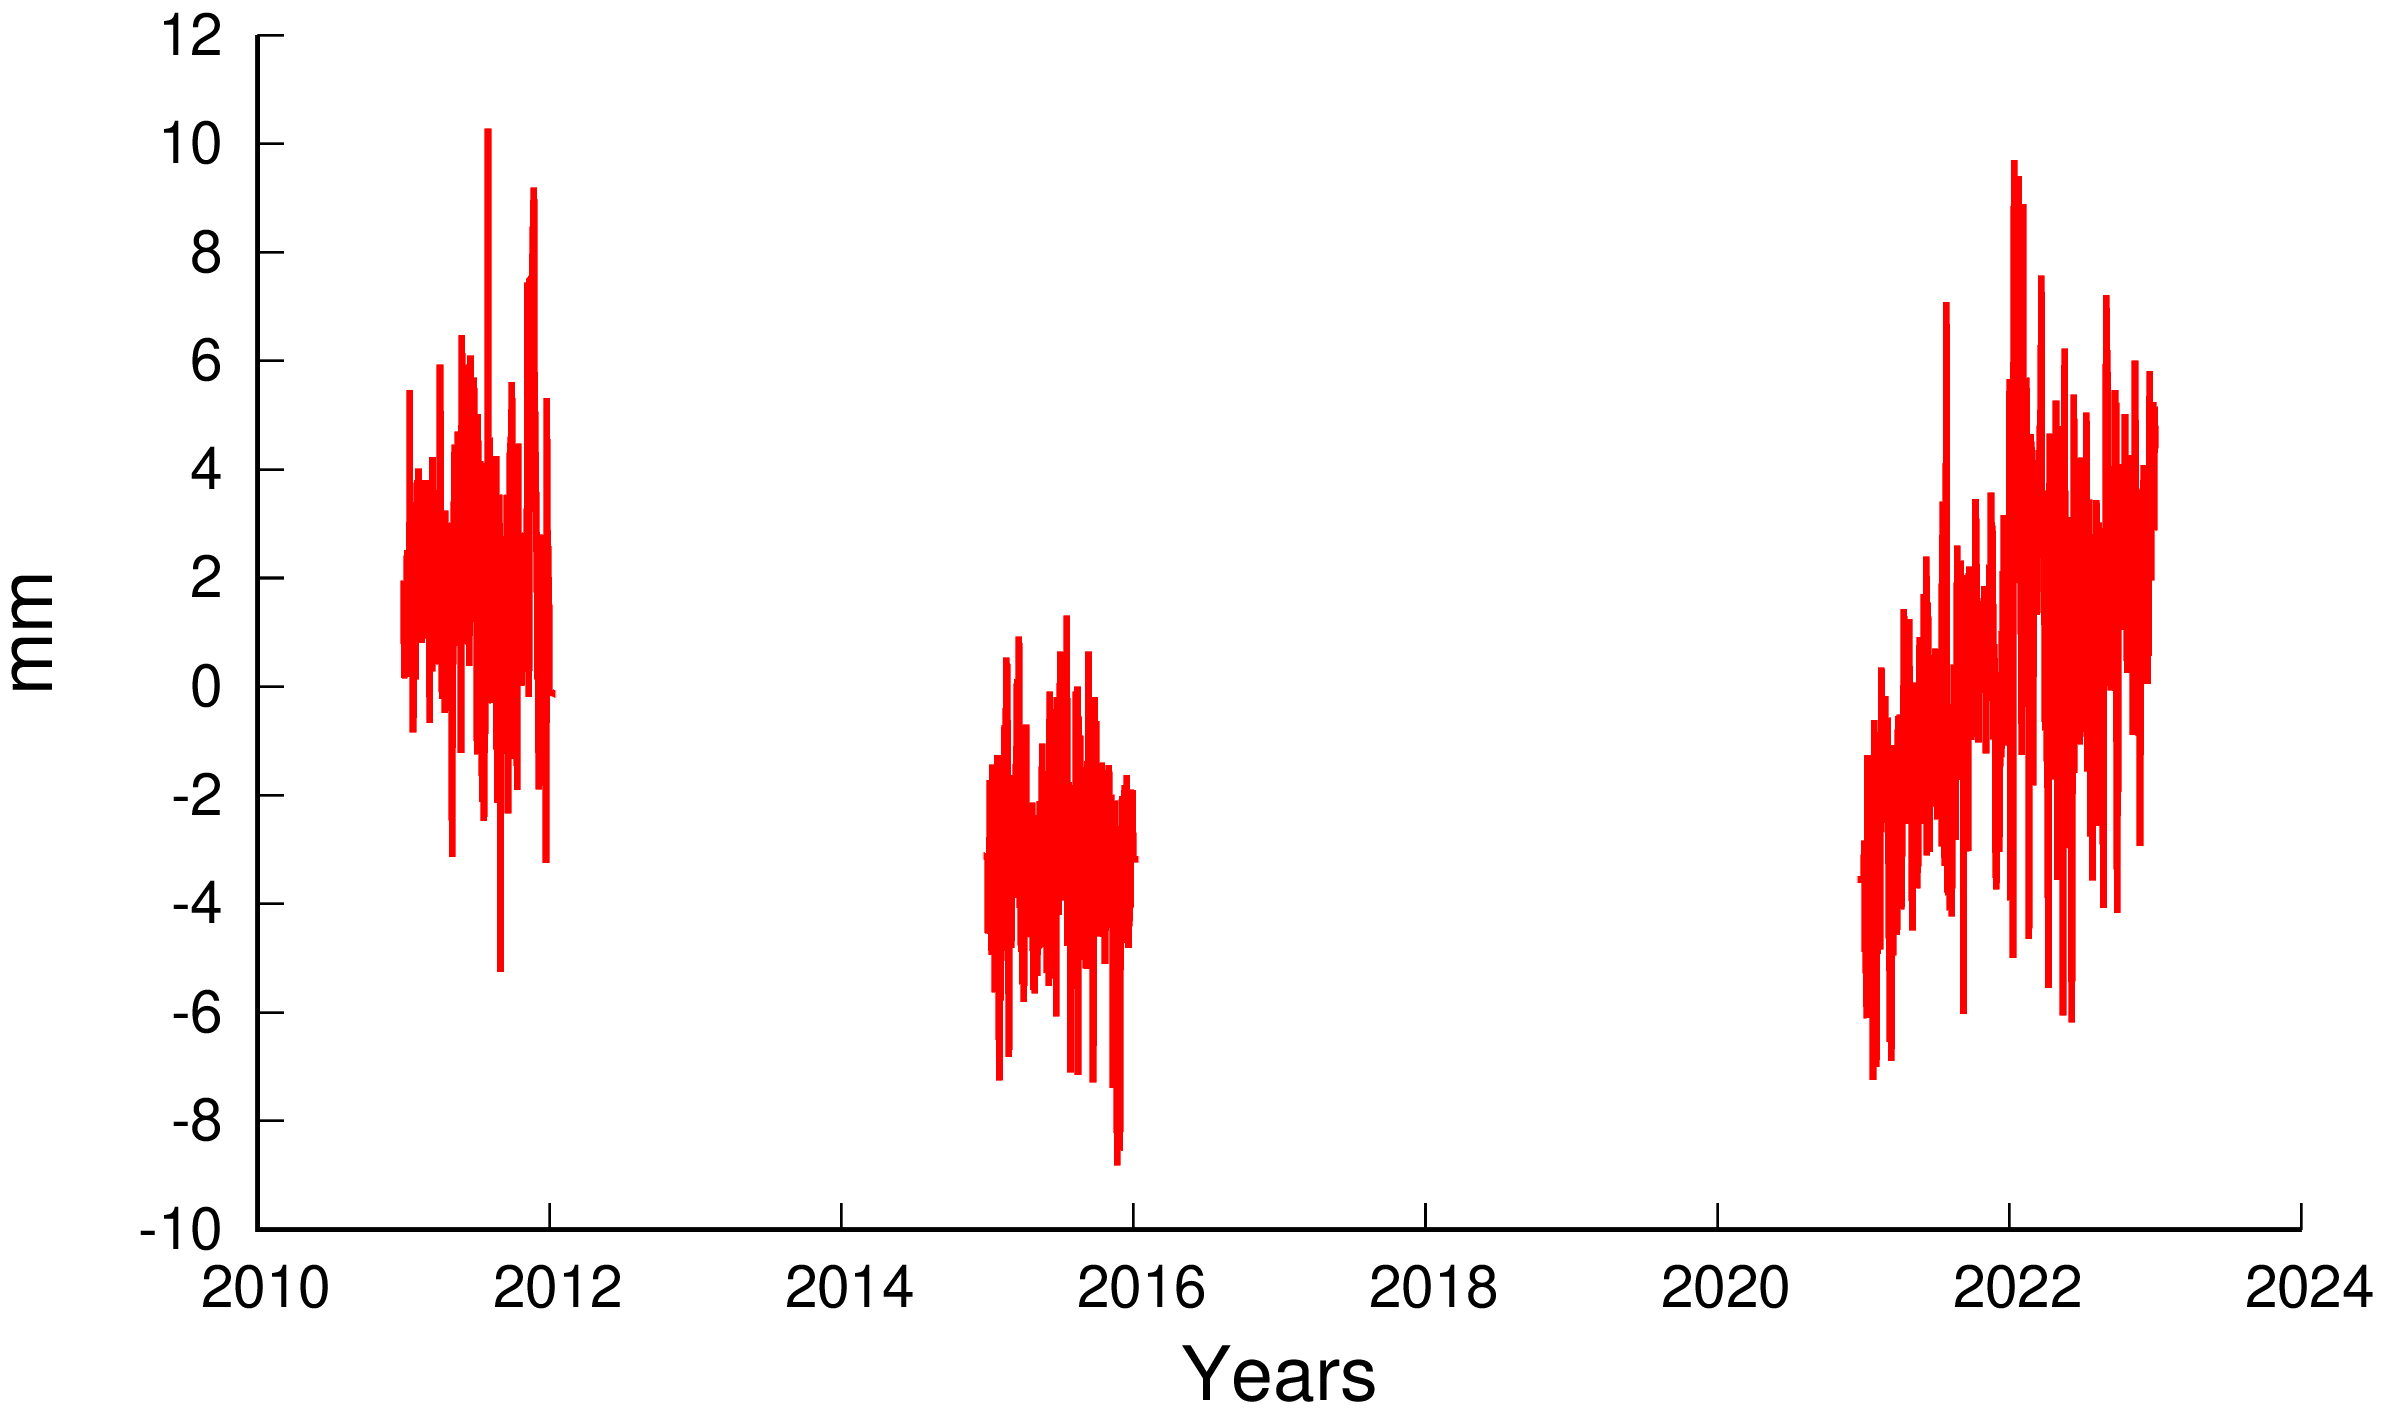
\includegraphics[height=5em]{057a_0_res.png}\\
  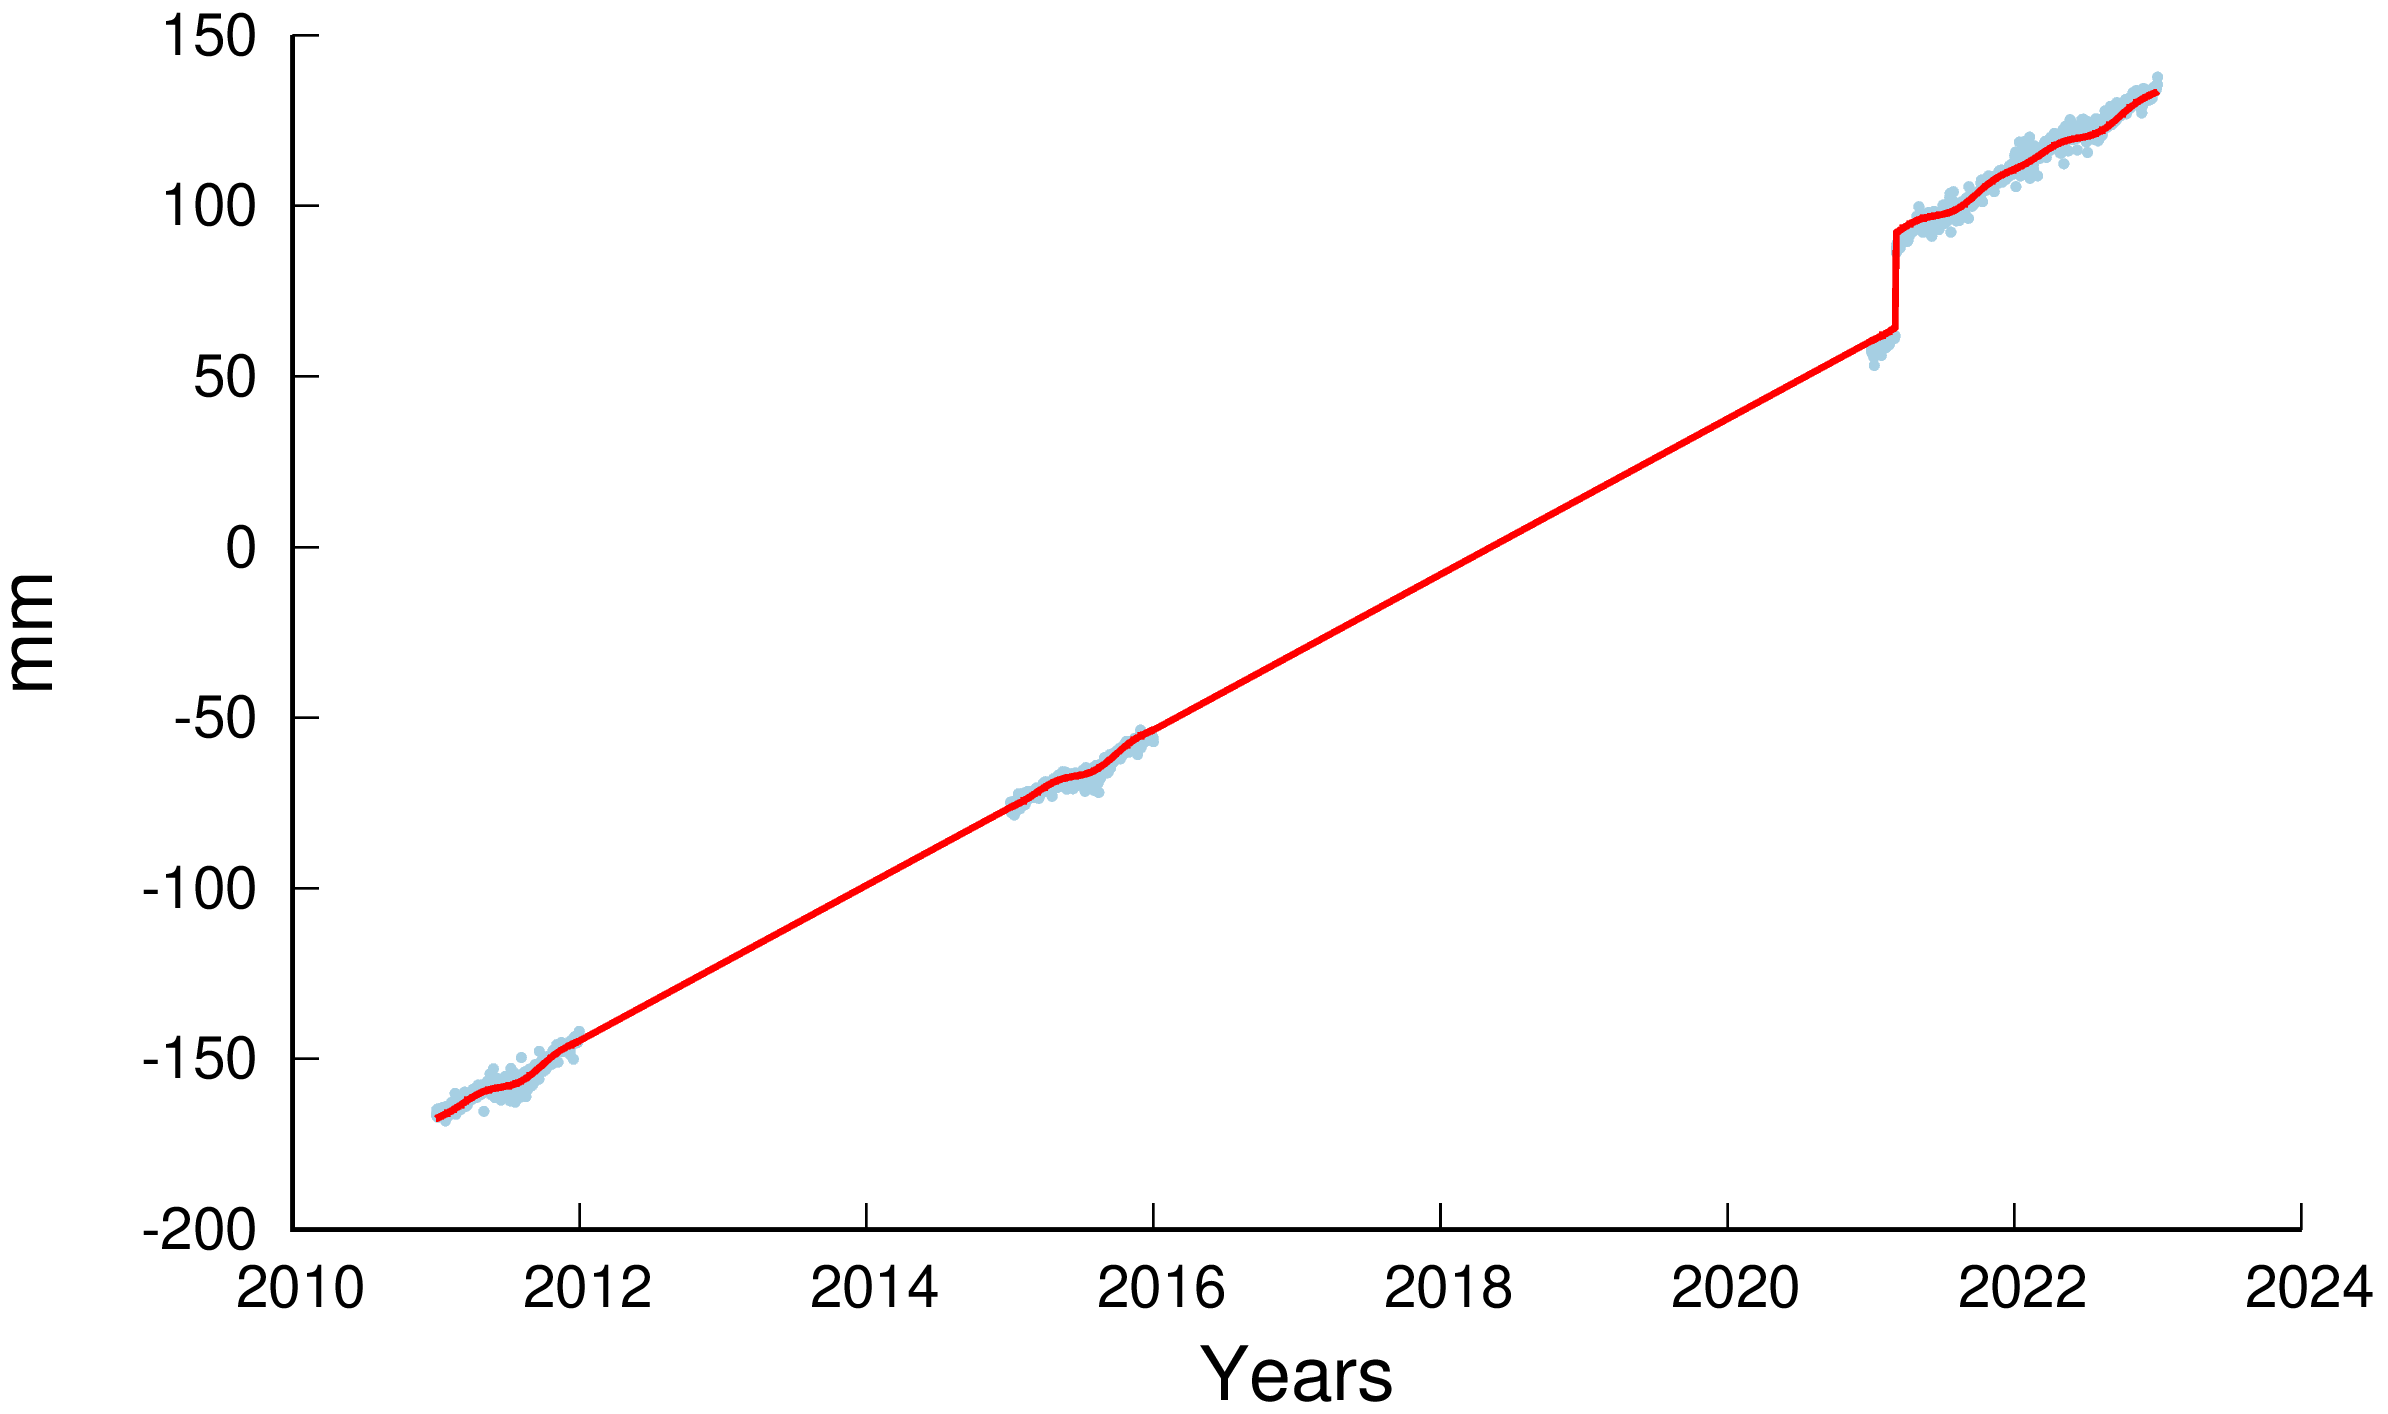
\includegraphics[height=5em]{057a_1_data.png}~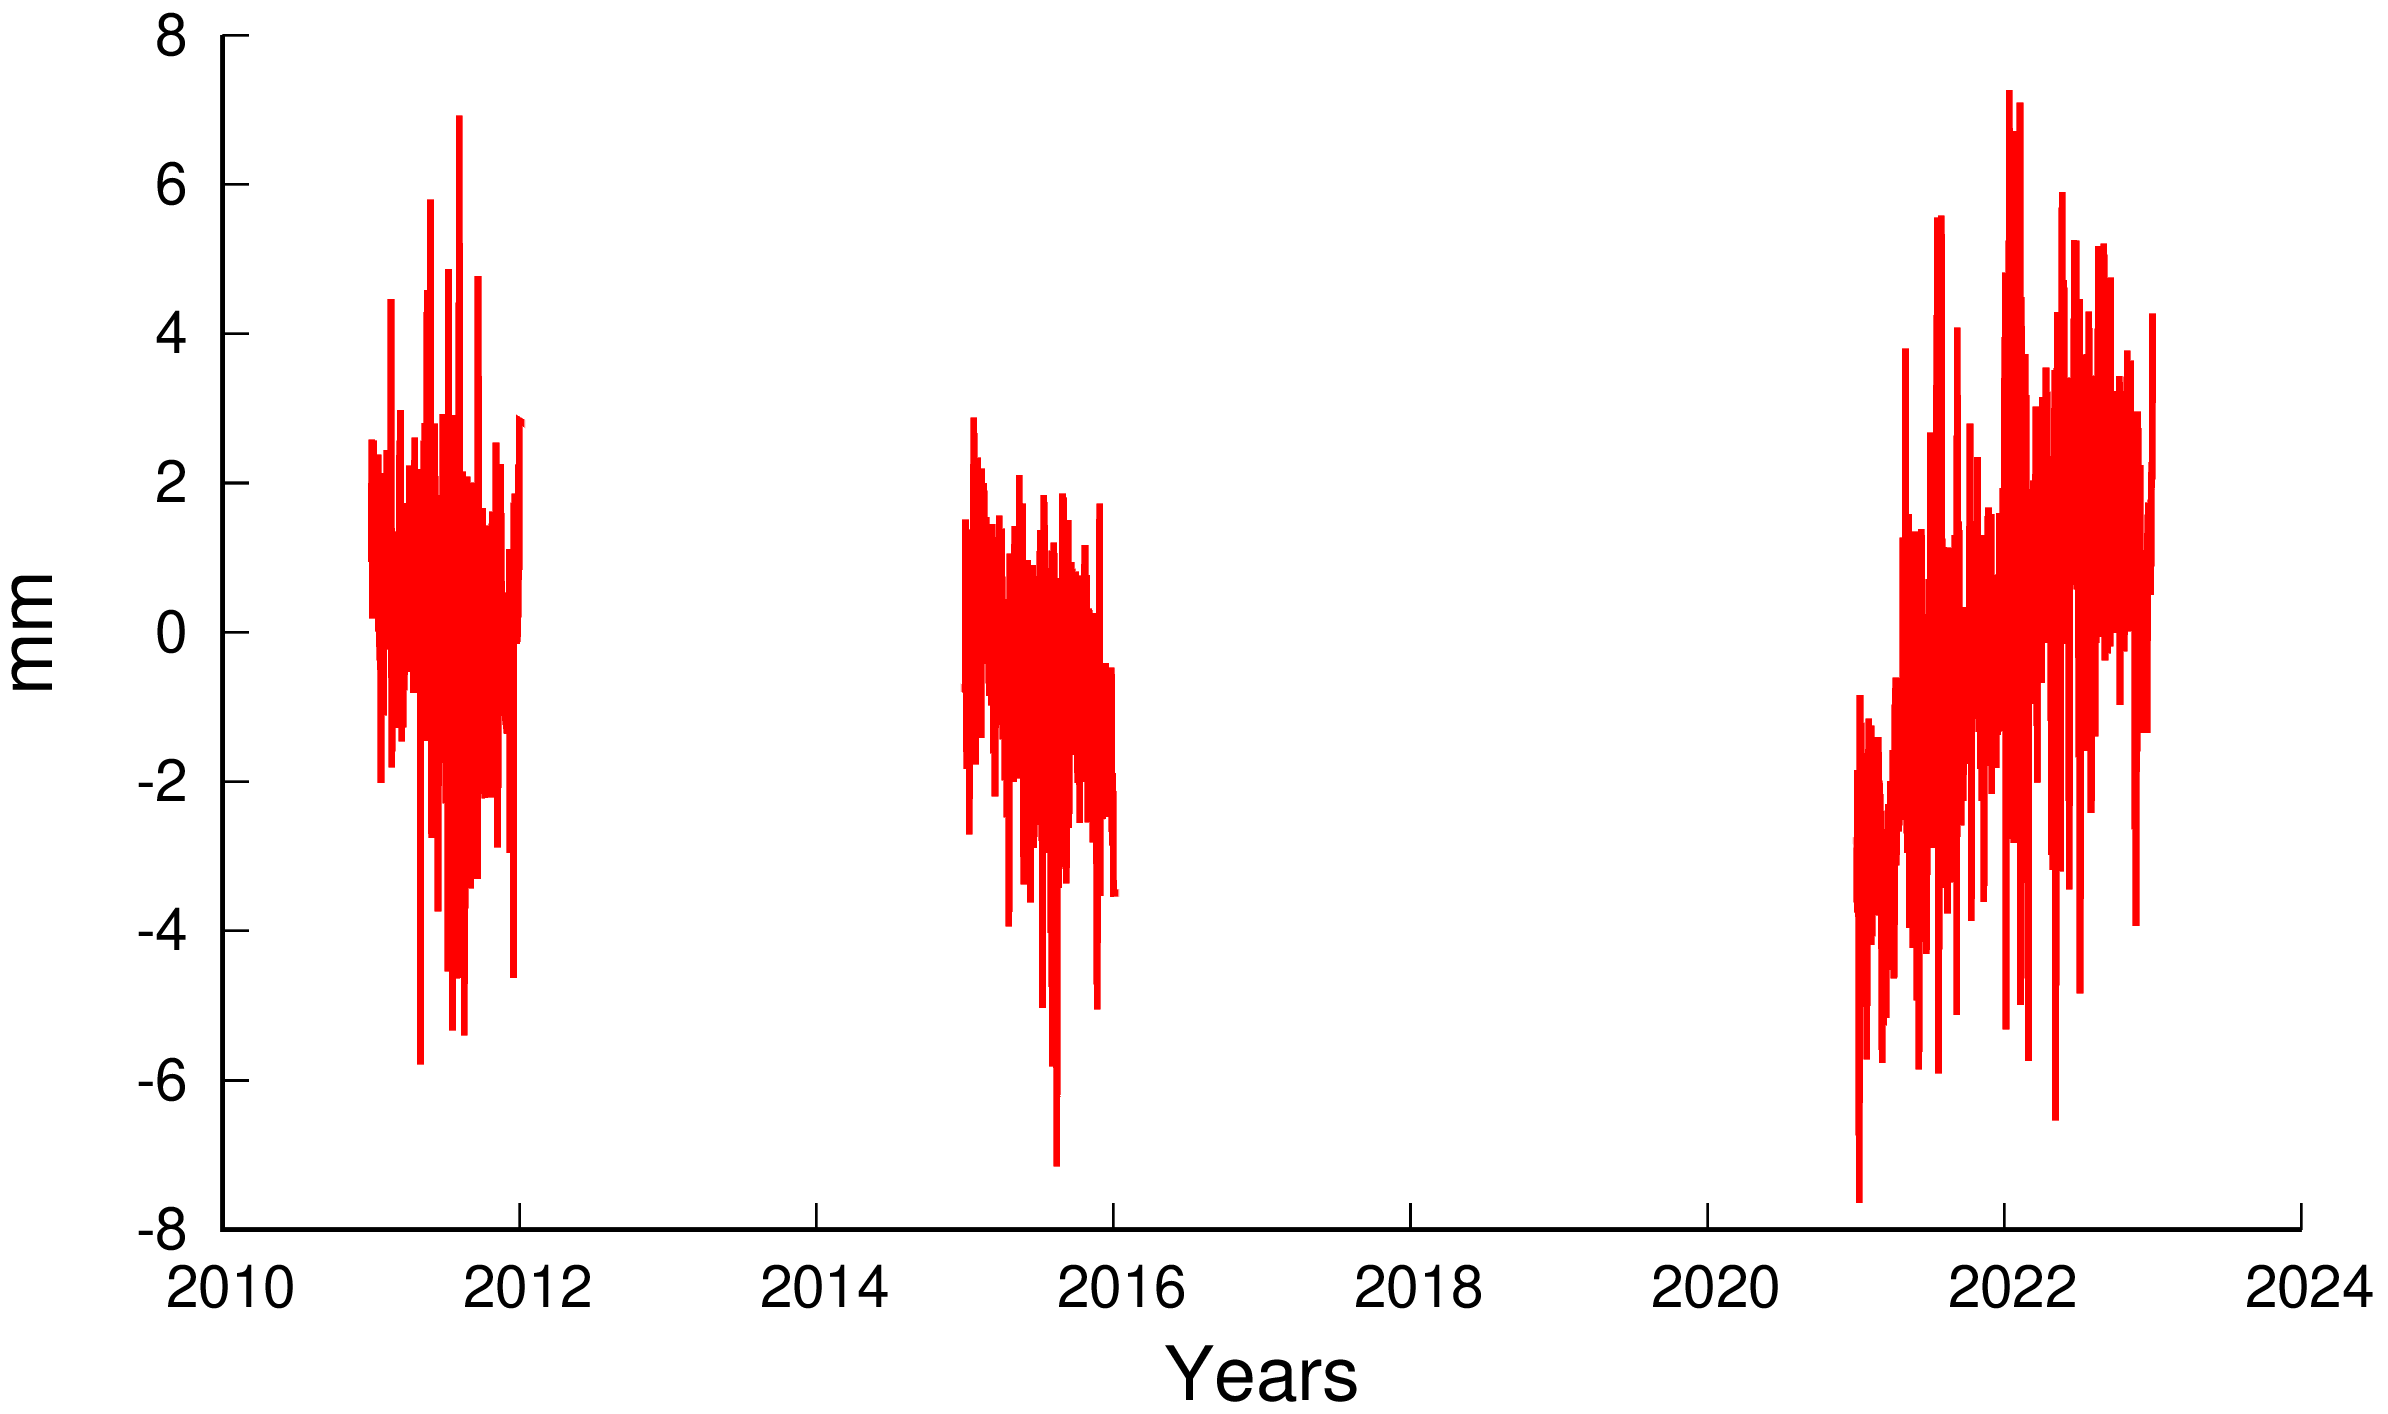
\includegraphics[height=5em]{057a_1_res.png}\\
  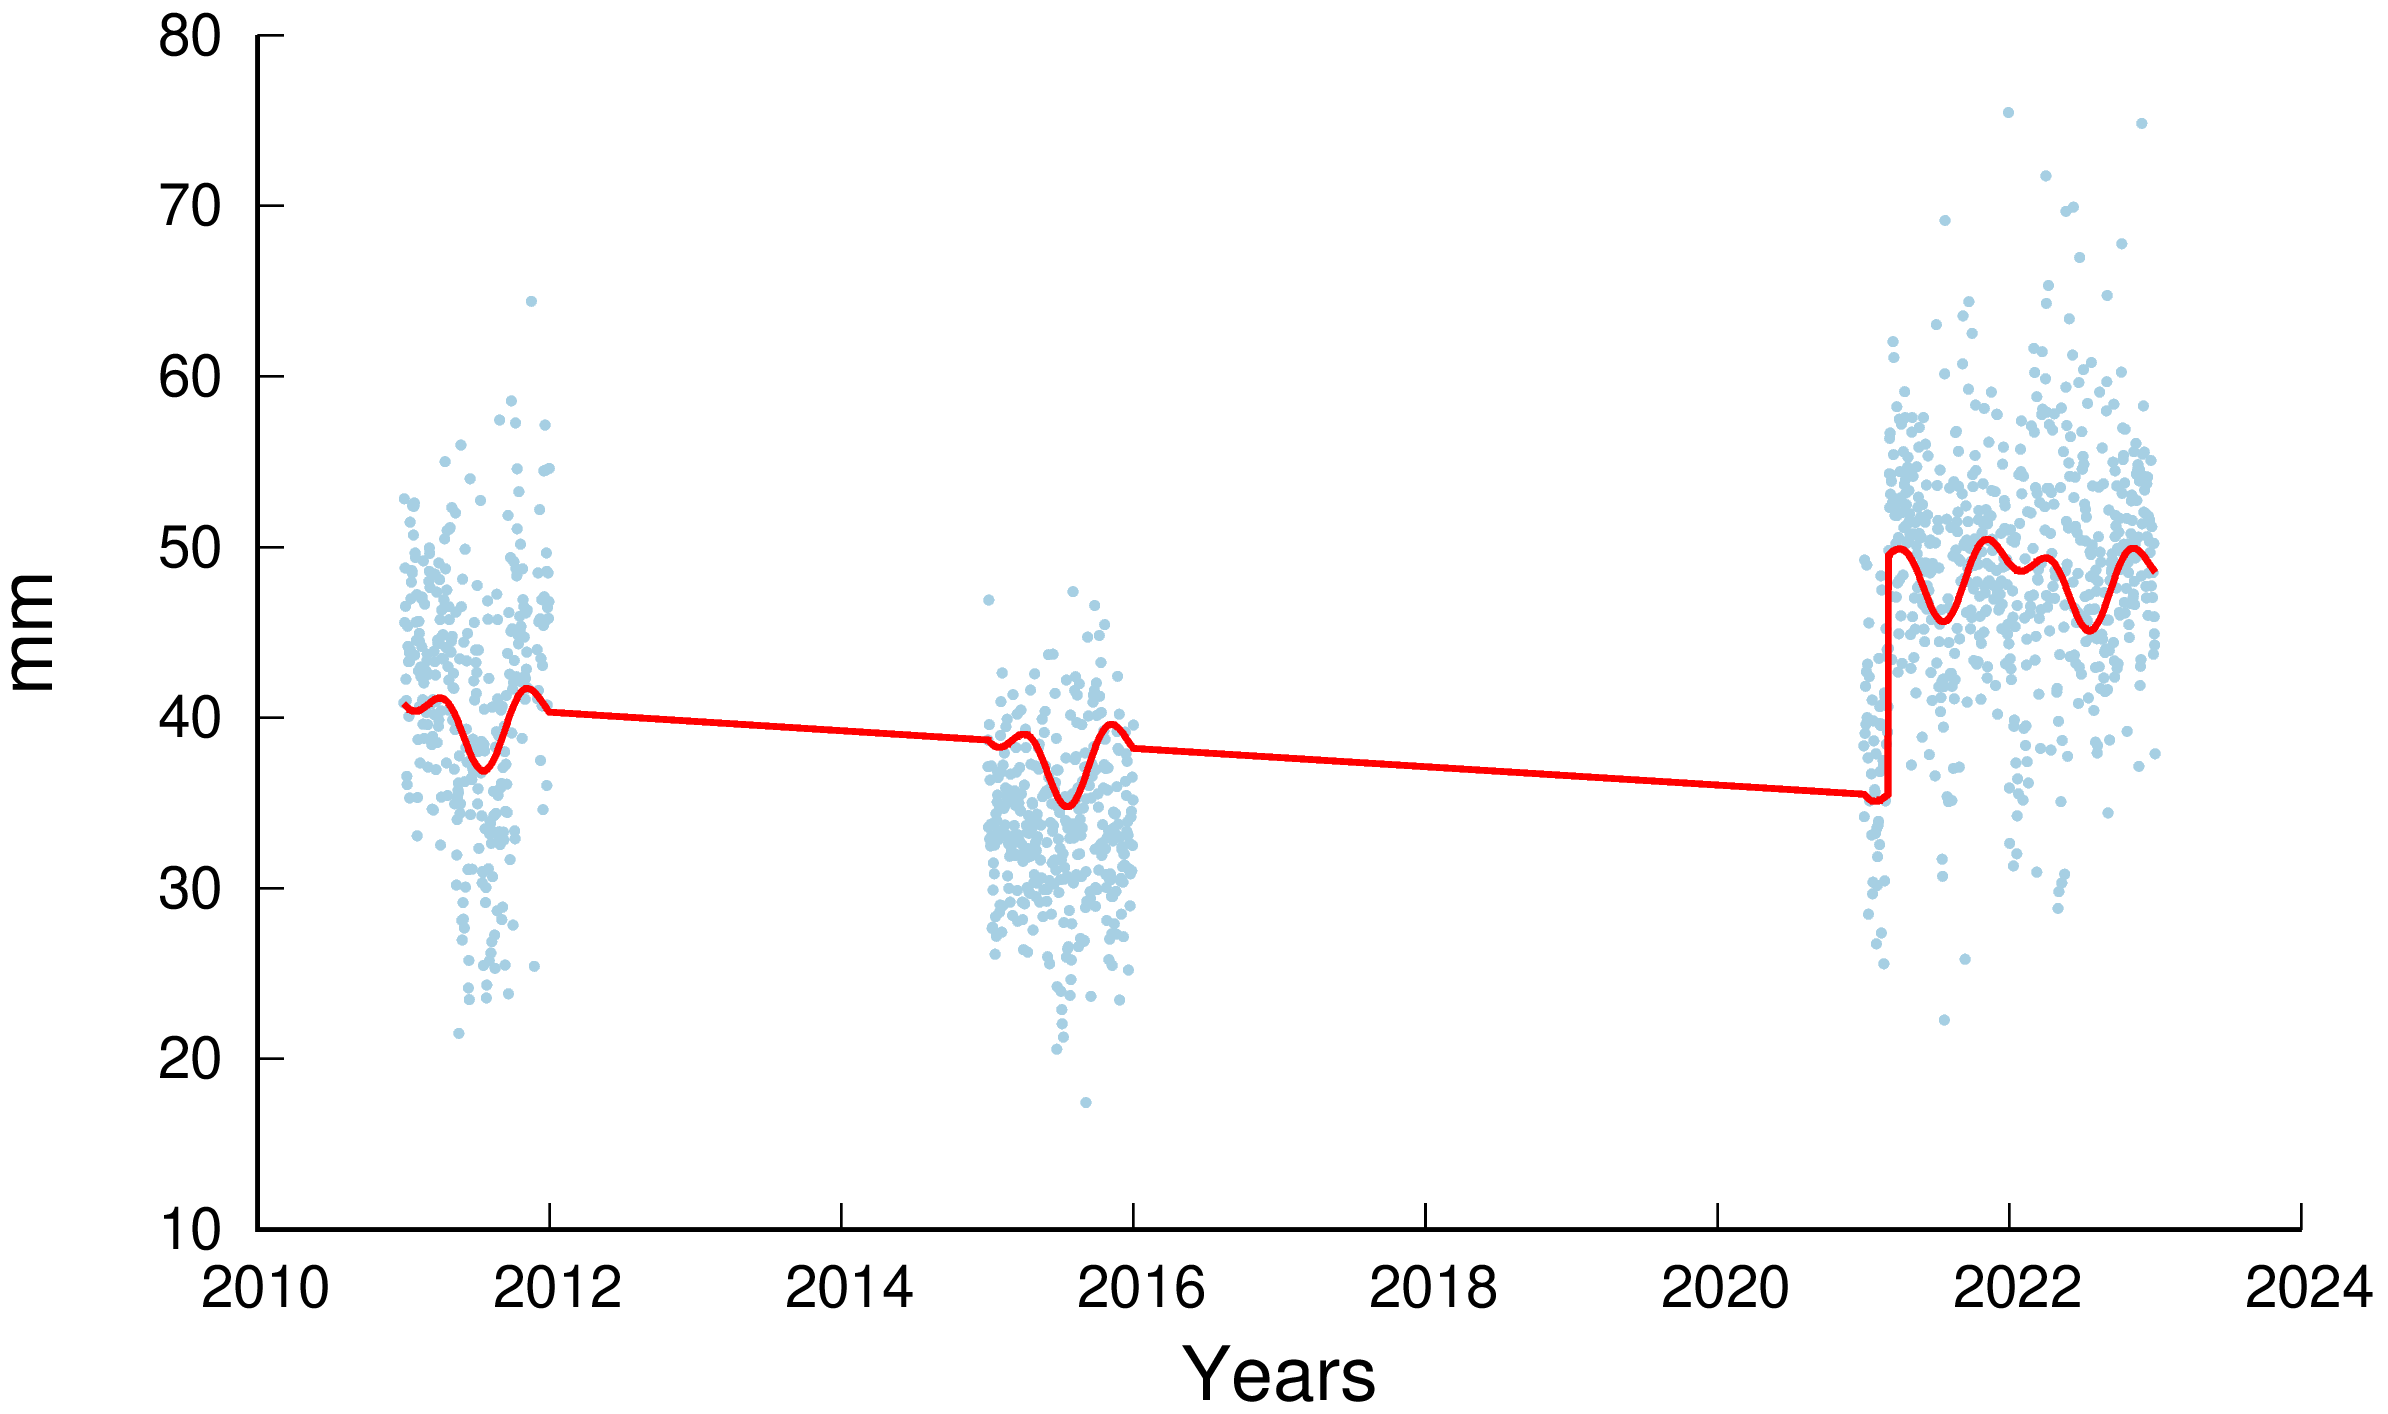
\includegraphics[height=5em]{057a_2_data.png}~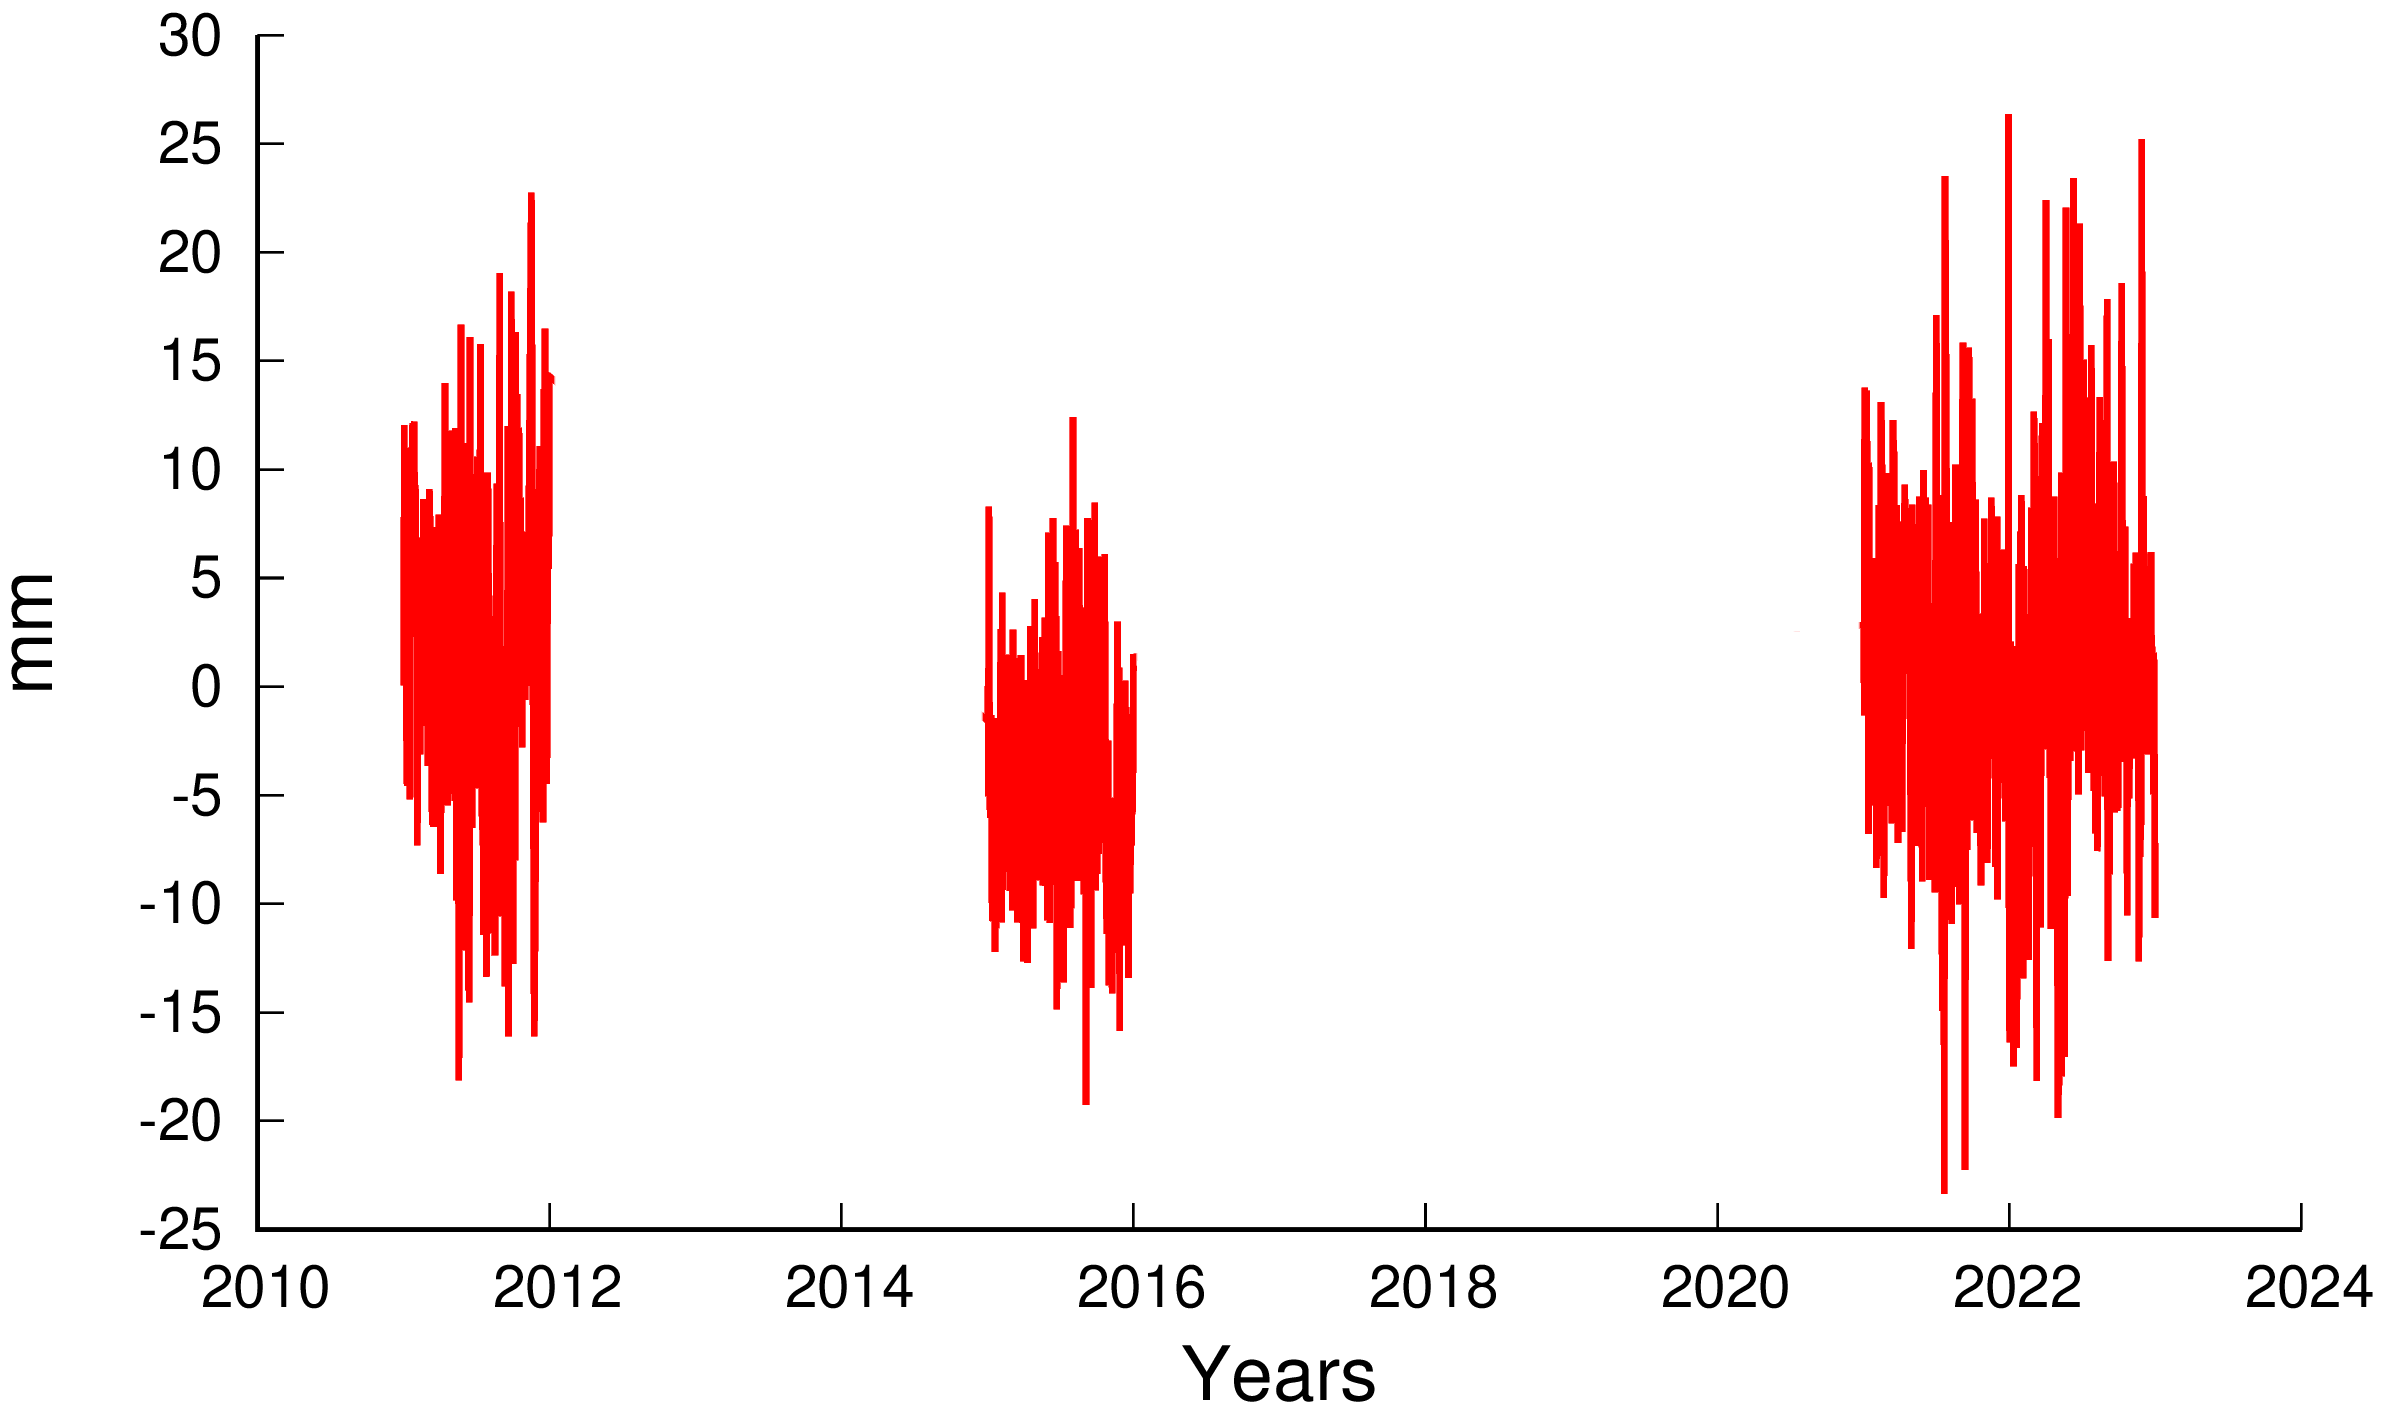
\includegraphics[height=5em]{057a_2_res.png}
\end{minipage}
\begin{minipage}[c]{0.33\linewidth}
\begin{center}
  040A (Santorini volcano inflation)
\end{center}
  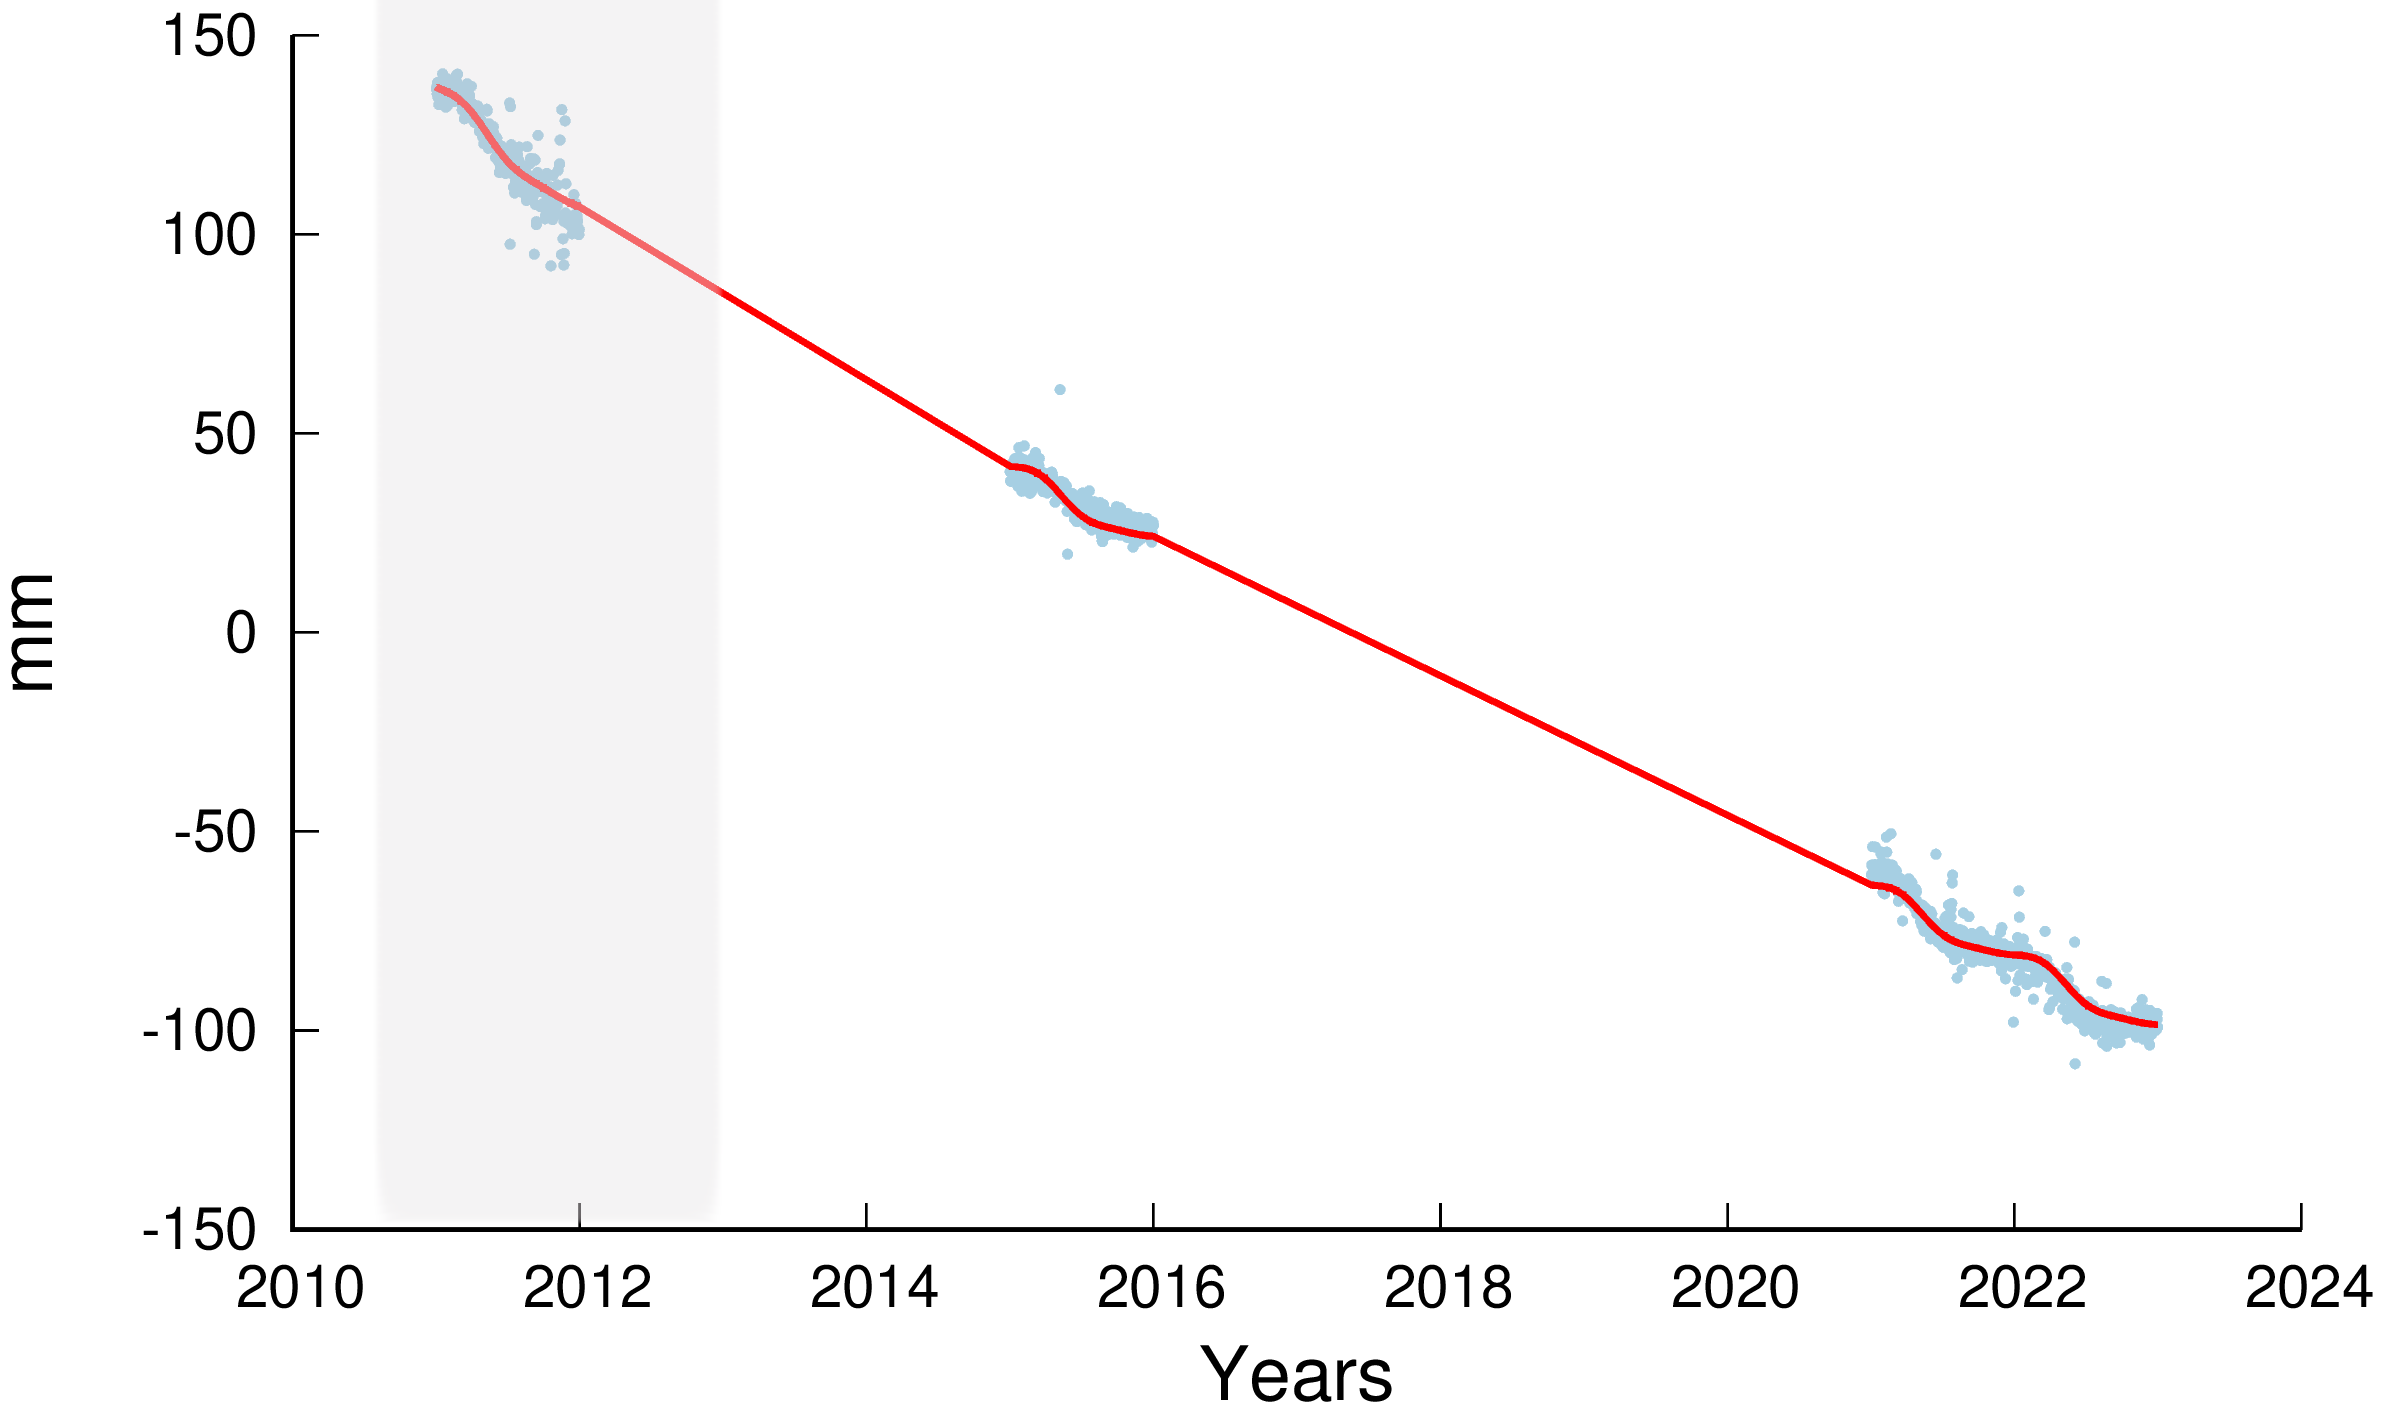
\includegraphics[height=5em]{048a_0_data.png}~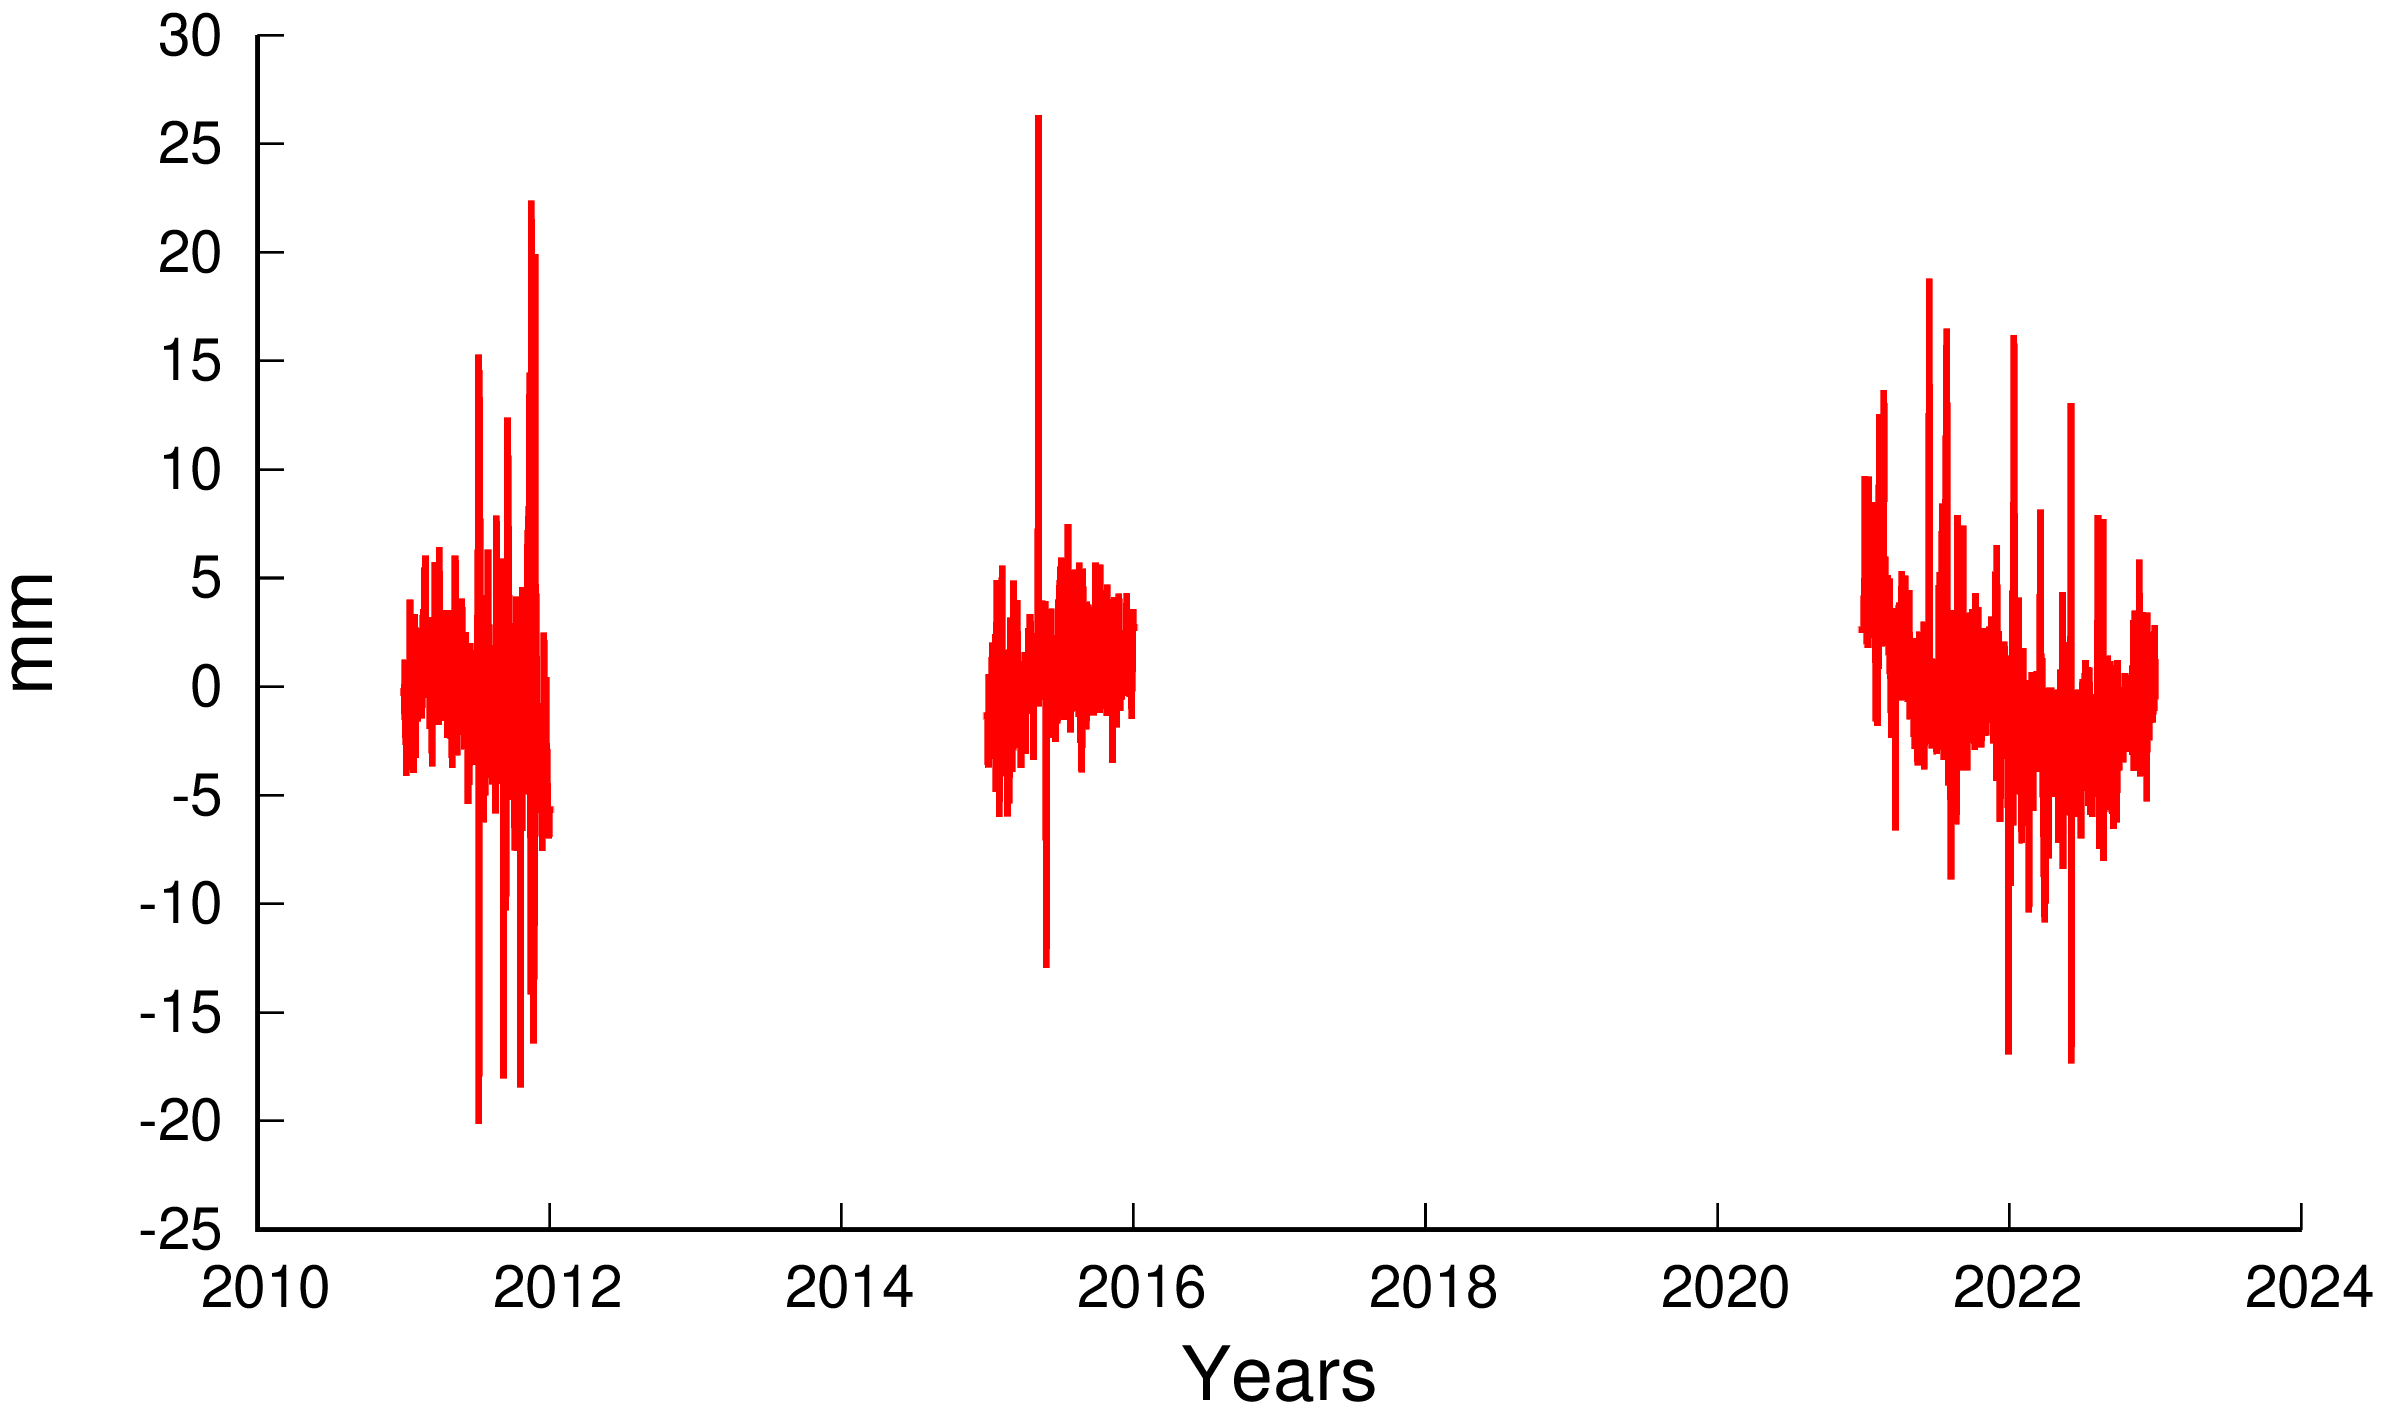
\includegraphics[height=5em]{048a_0_res.png}\\
  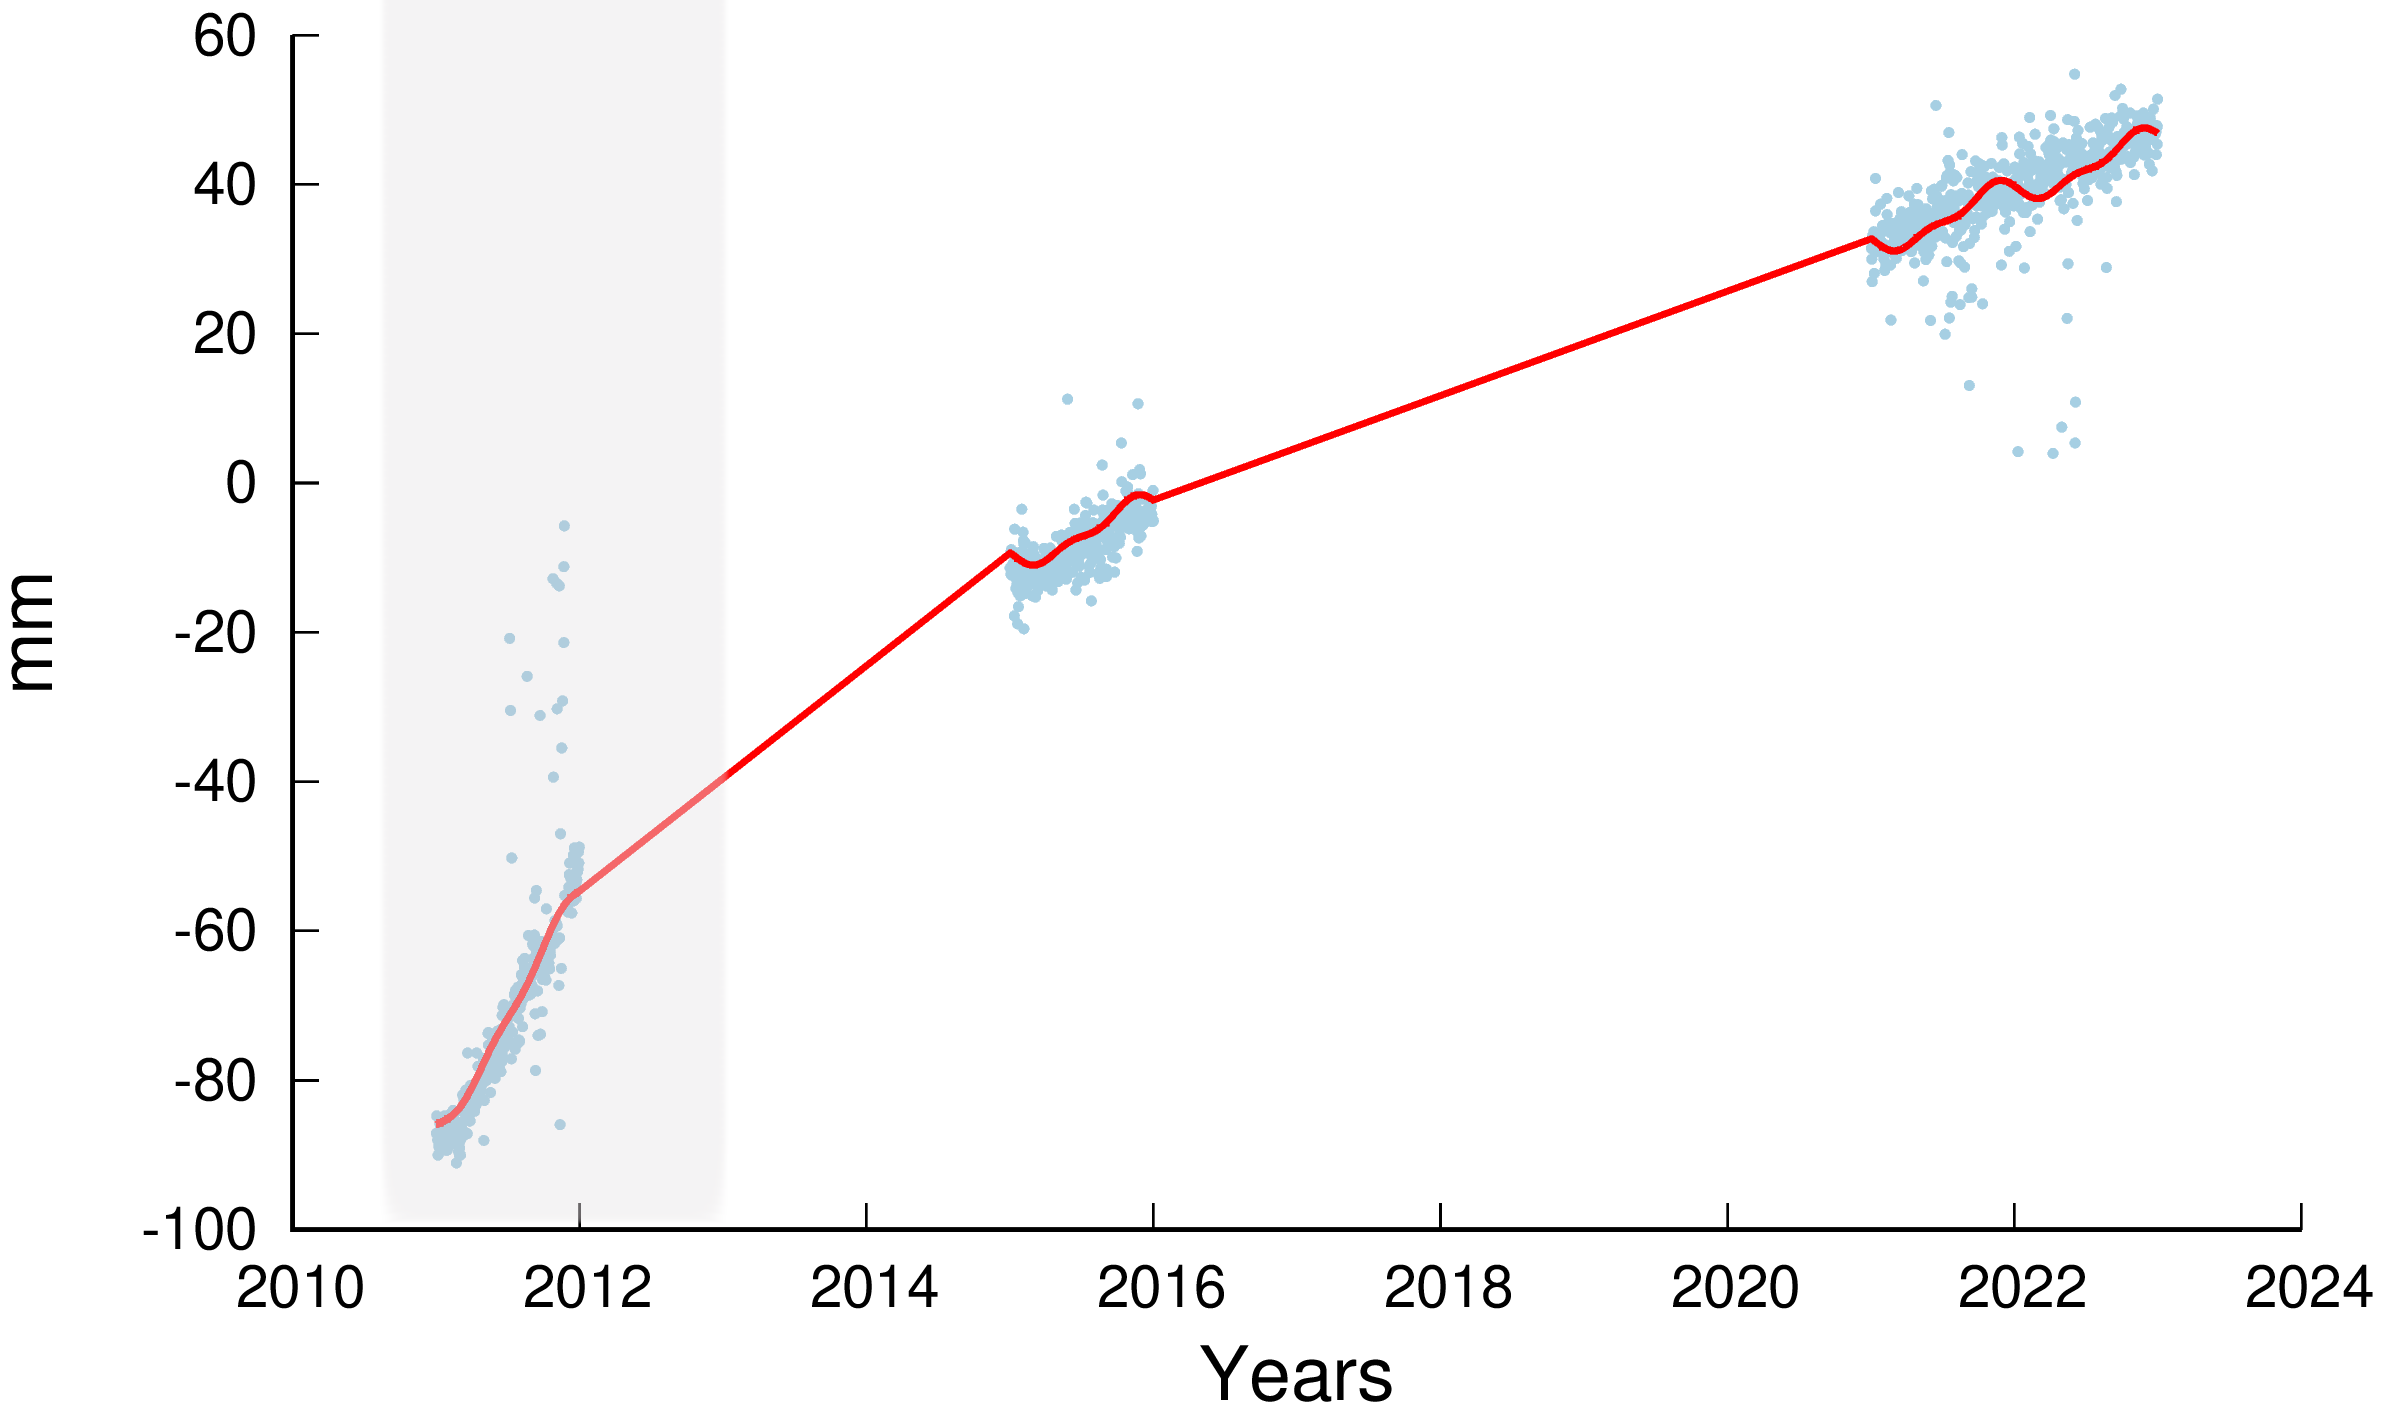
\includegraphics[height=5em]{048a_1_data.png}~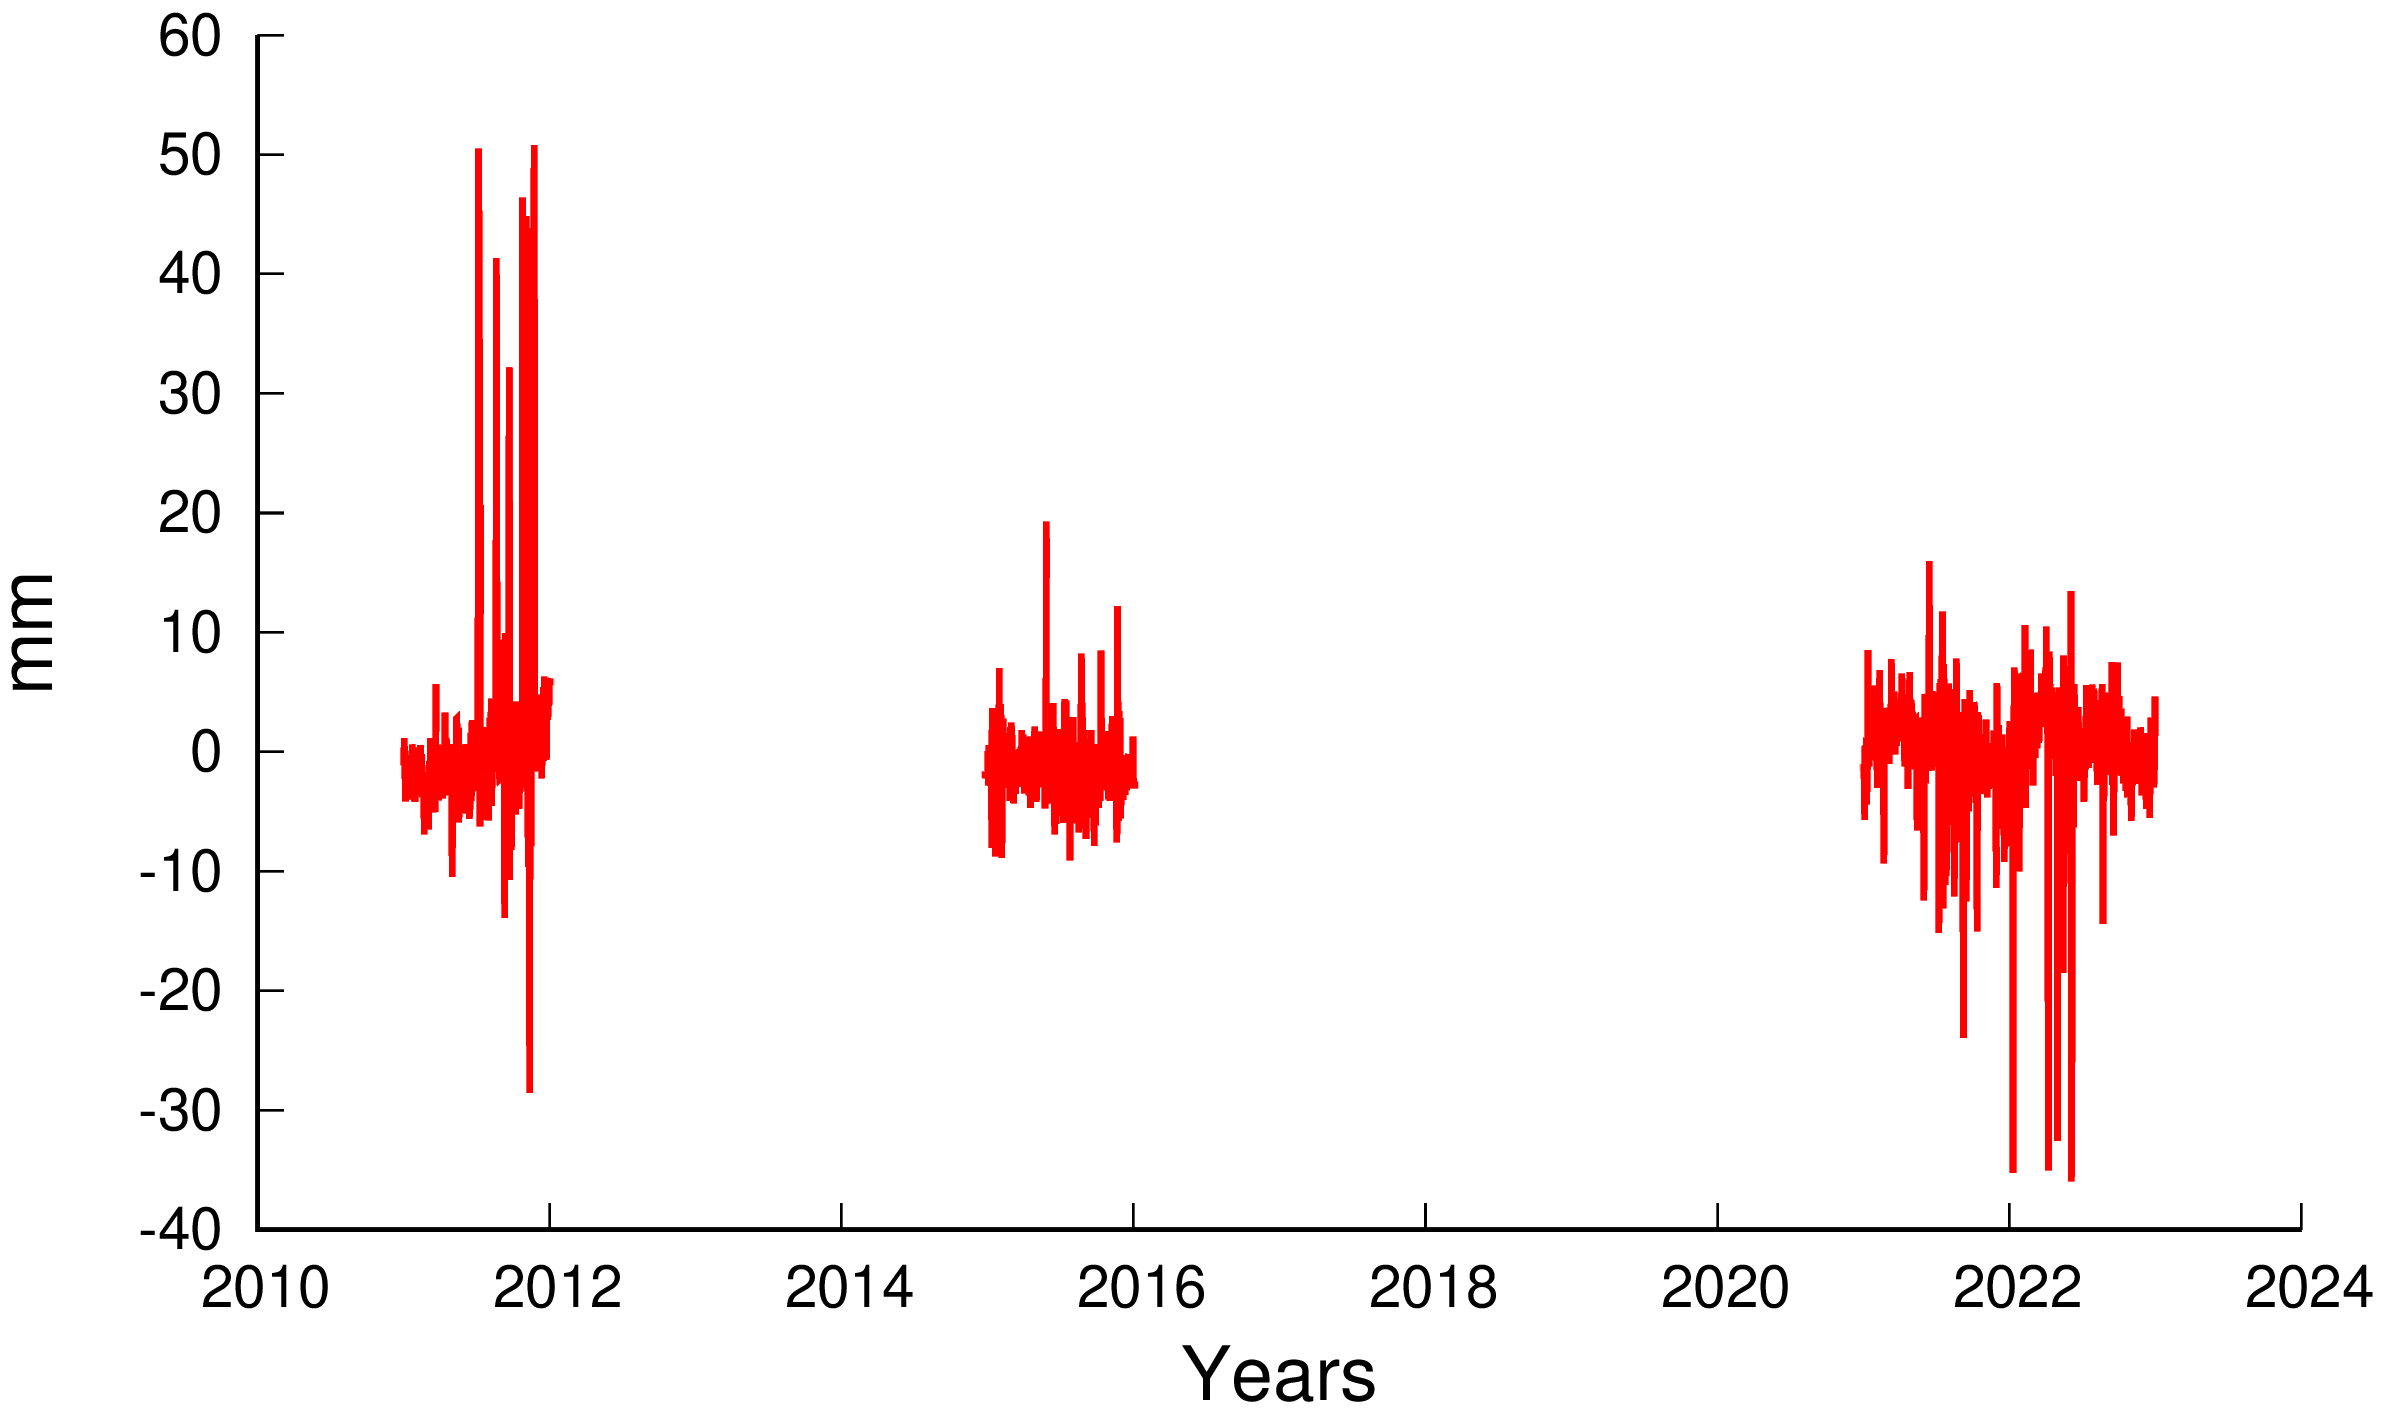
\includegraphics[height=5em]{048a_1_res.png}\\
  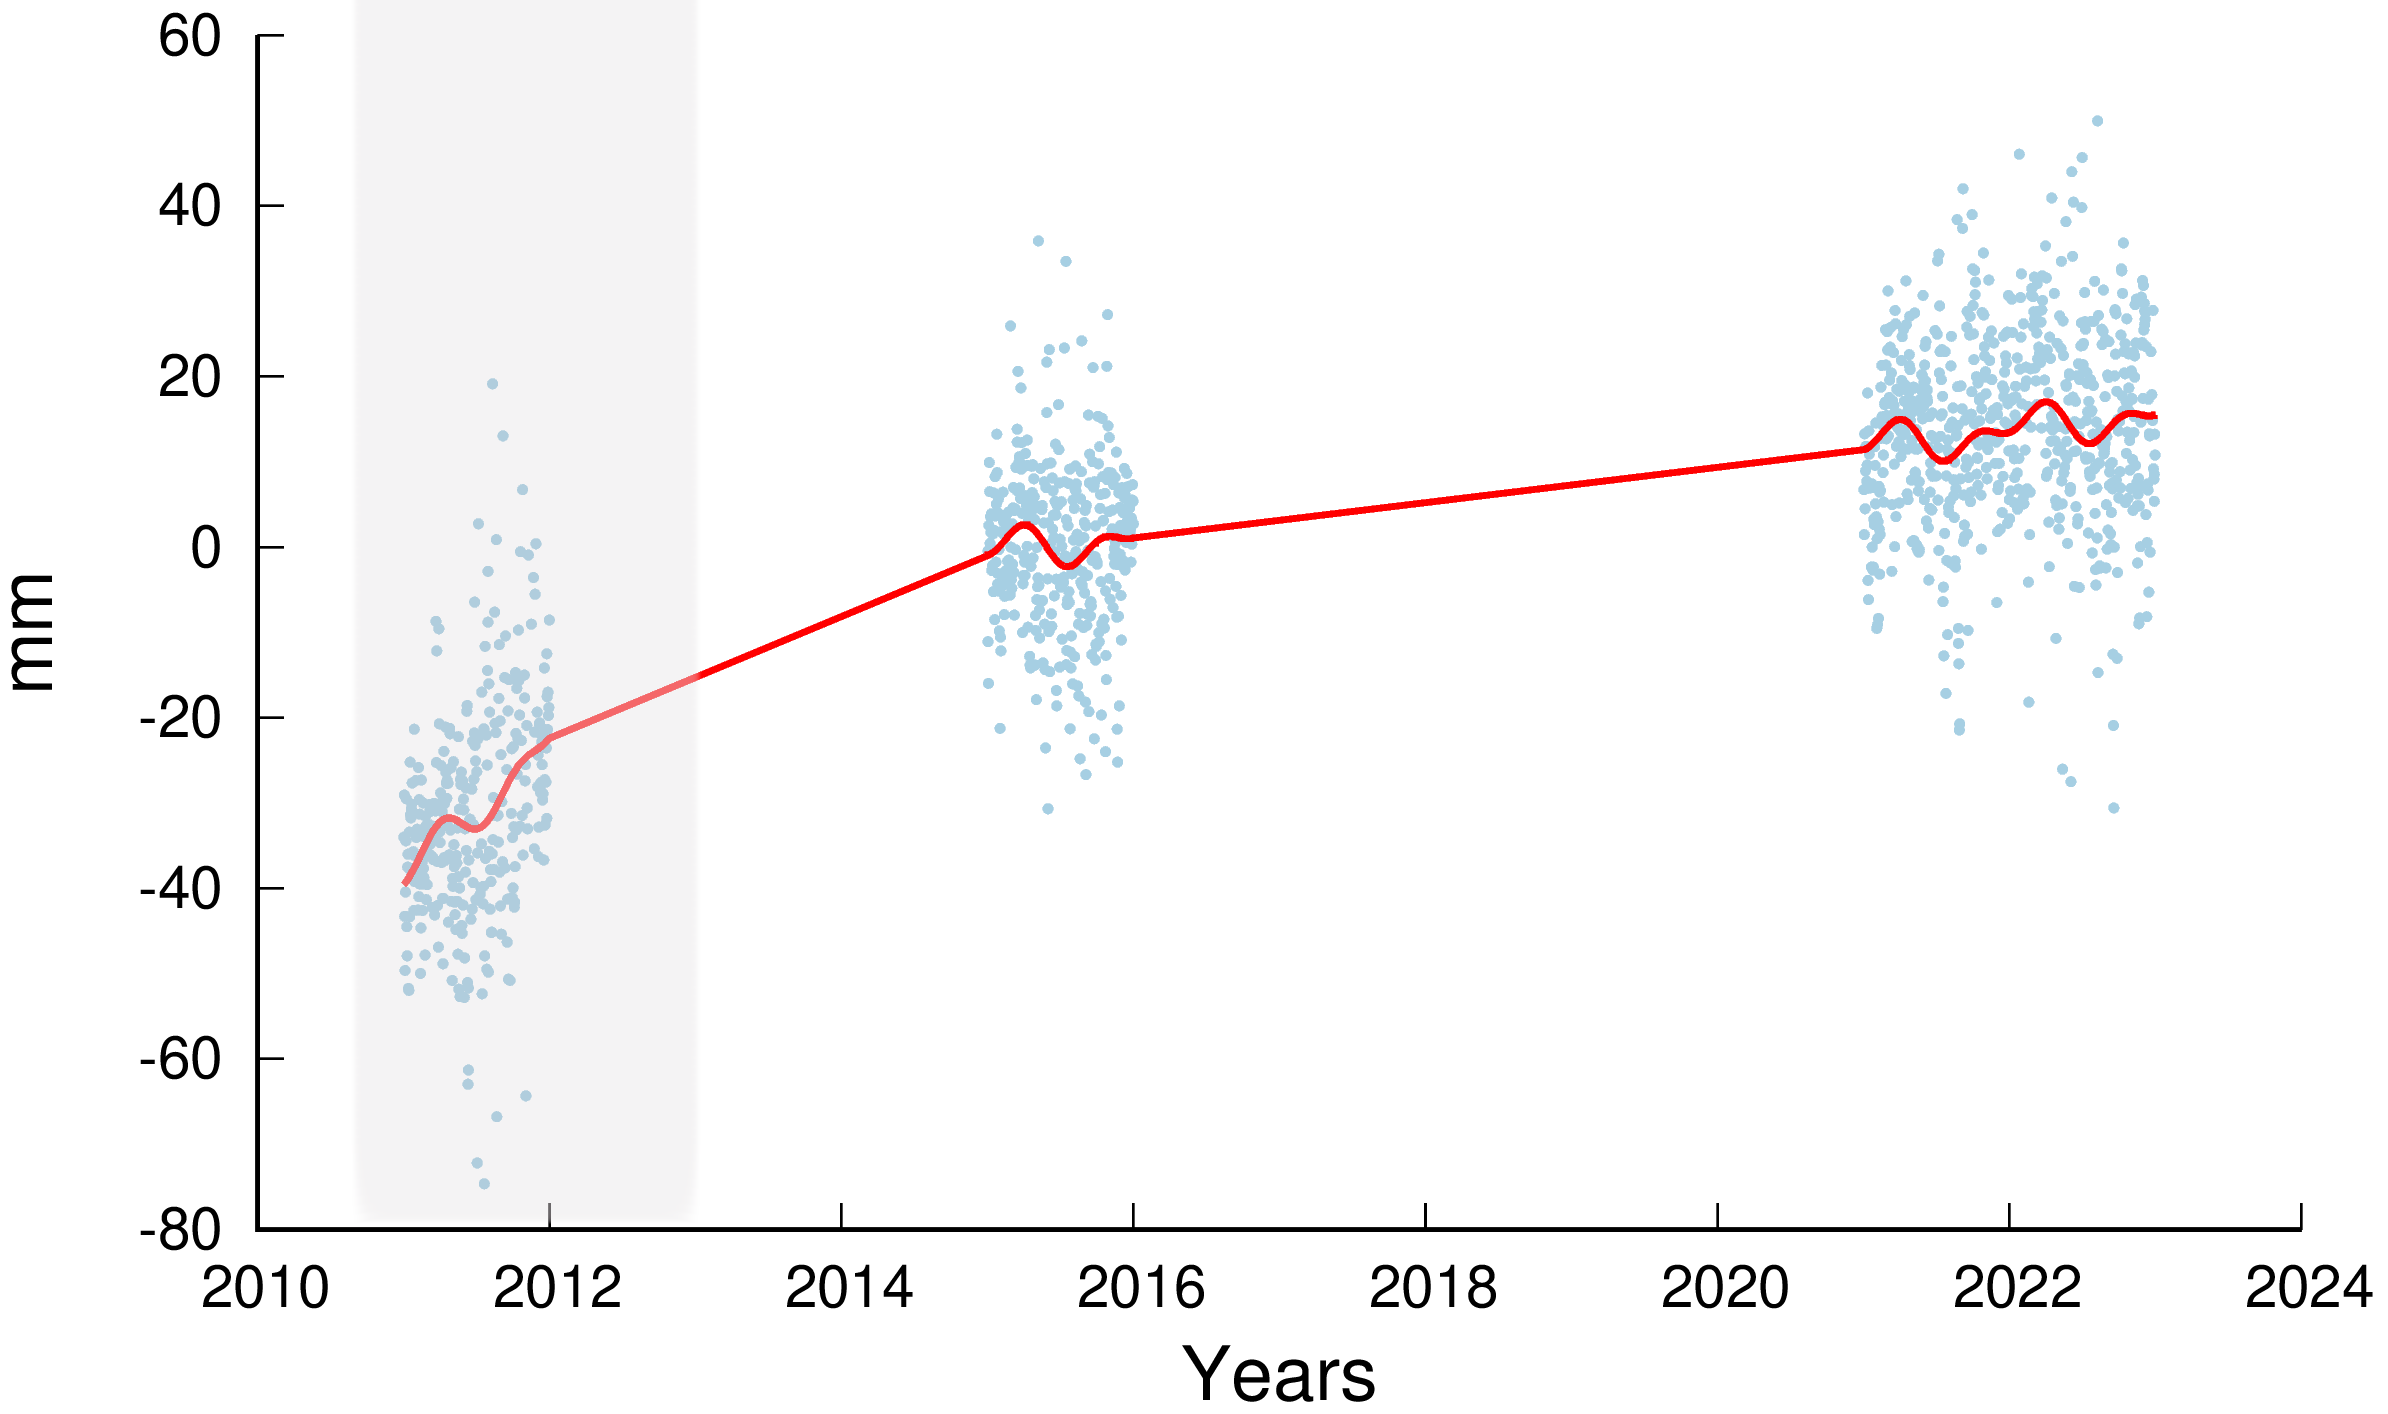
\includegraphics[height=5em]{048a_2_data.png}~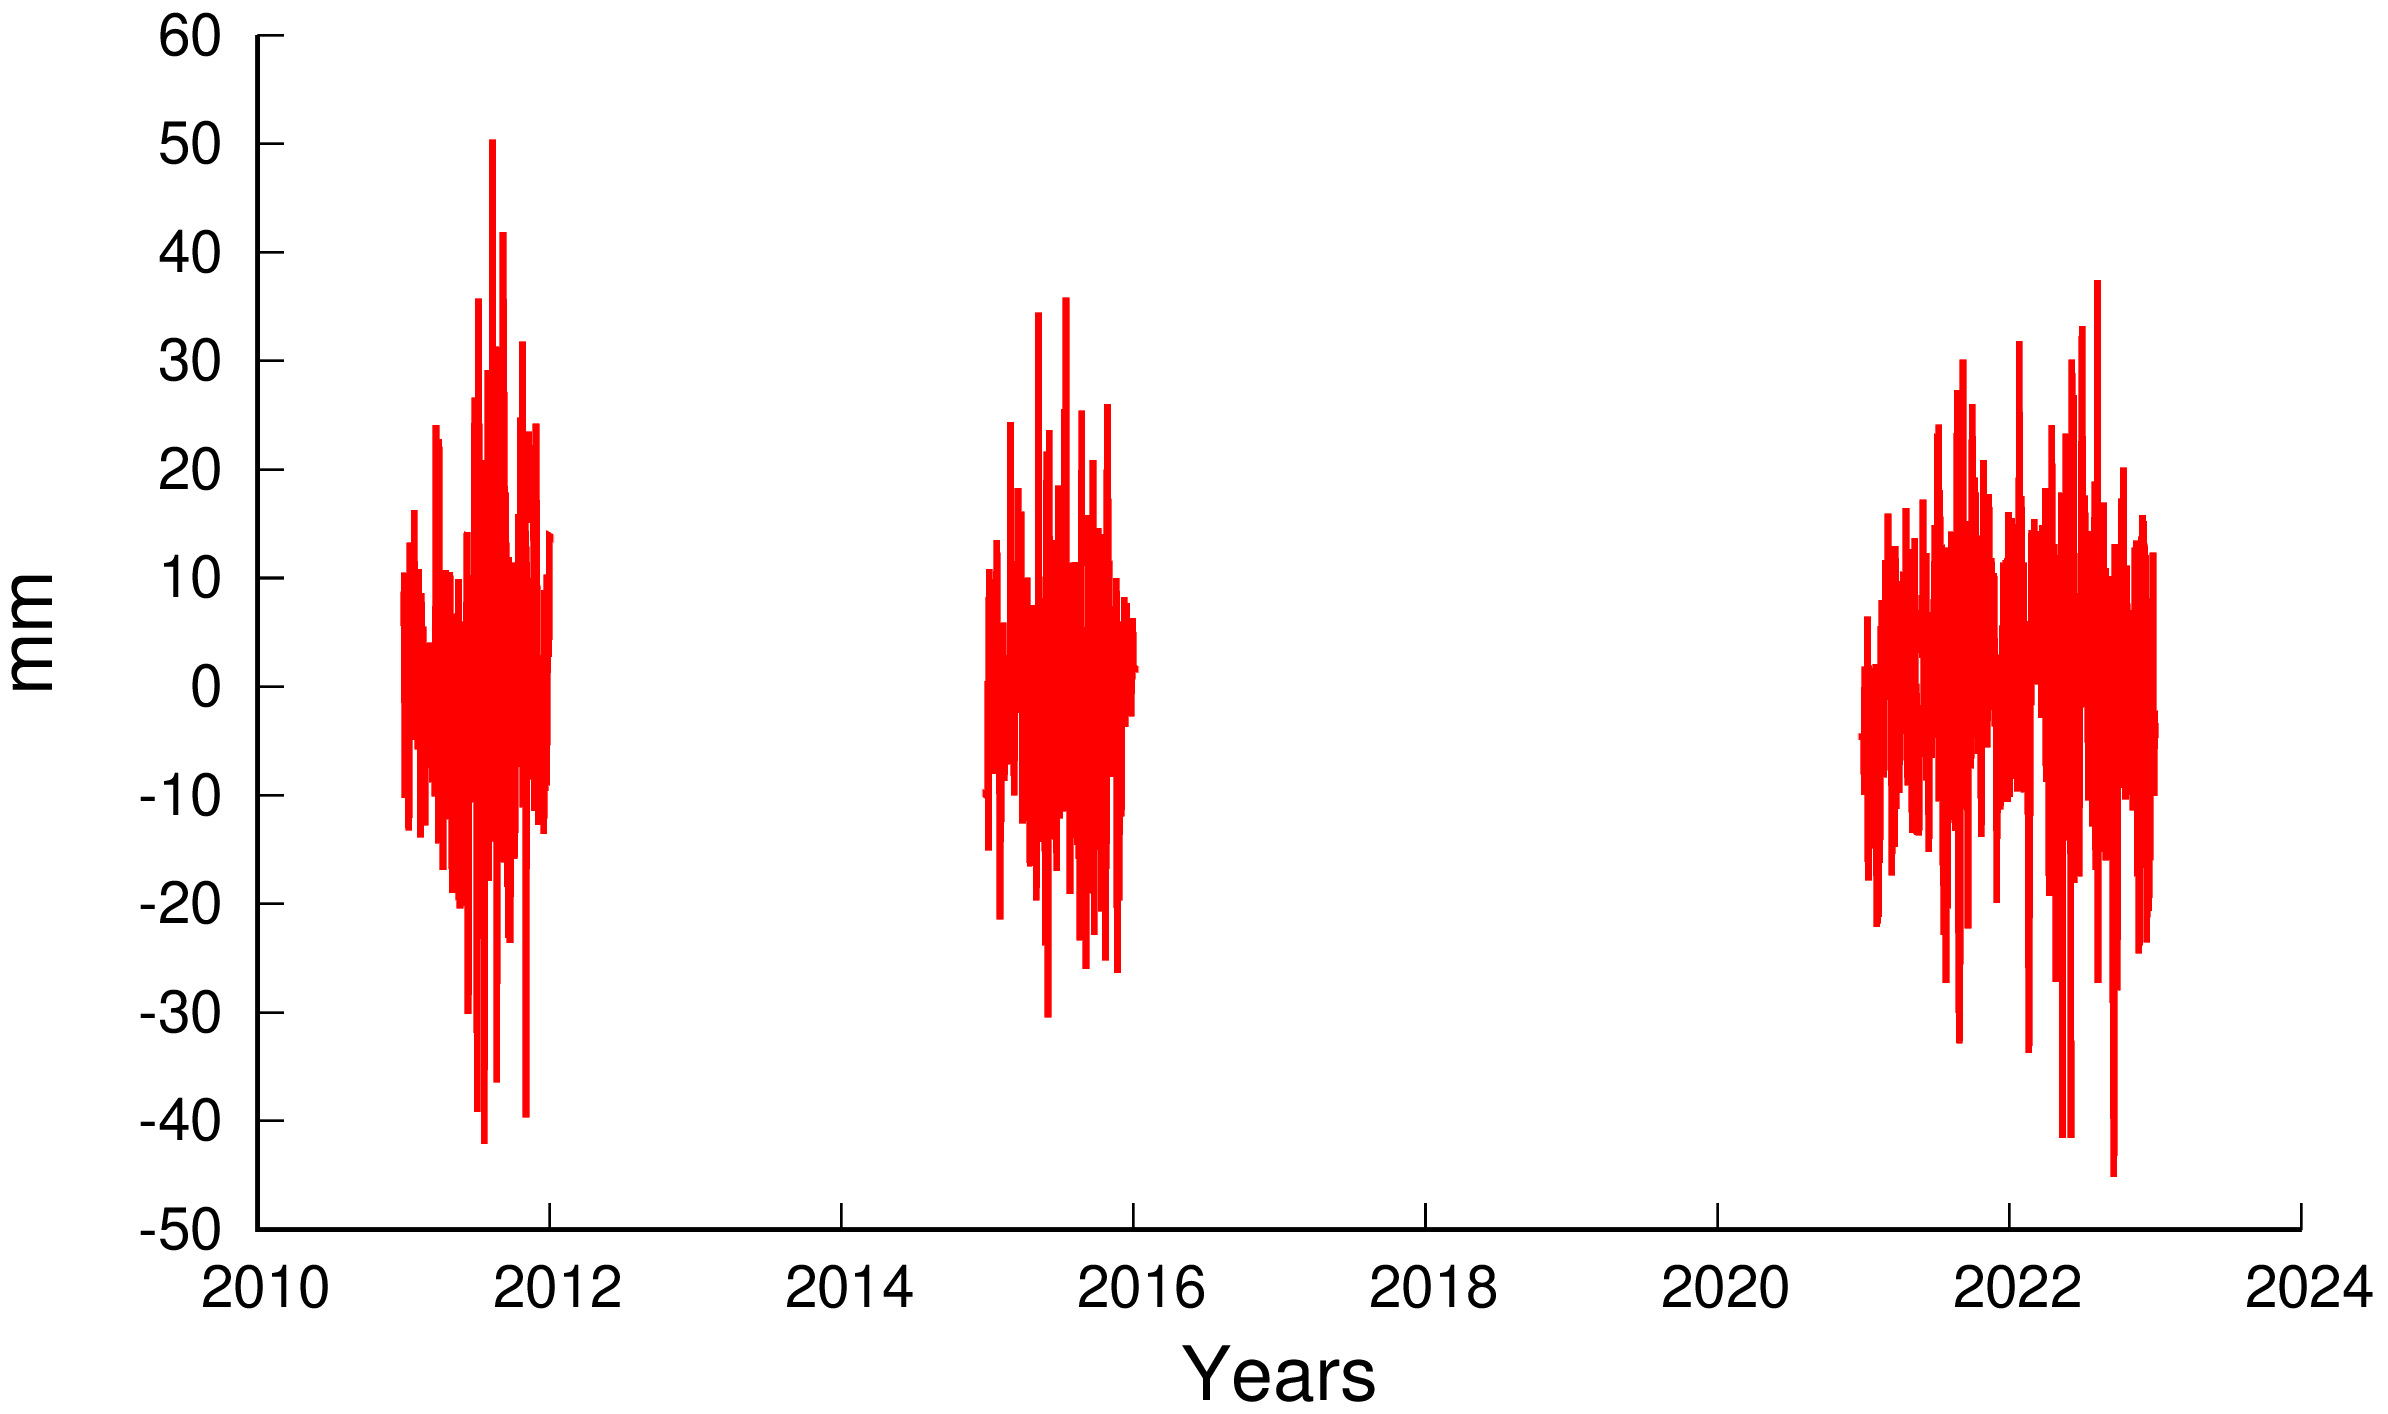
\includegraphics[height=5em]{048a_2_res.png}
\end{minipage}
%\begin{minipage}[c]{0.71\linewidth}
%%A total number of 302 GNSS stations belonging to the EUREF Permanent Network (EPN) 
%%were selected on the basis of the following criteria: 
%%a) station have an observation period longer than 3 years,
%%b) only one velocity solution is computed per station and
%%c) stations with large velocity changes excluded.
%%The station positions are estimated using several geodetic software packages and 
%%in a second step then CATREF software was used to estimate multi-year position 
%%and velocity solutions. The available dataset comprises the velocity field 
%%extracted from the C2010 EPN solution.
%%
%%The reference frame of the velocity field is ETRF2014 which is the realization 
%%of ETRS89 corresponding to ITRF2014. According to EUREF Technical Report 1, the 
%%ETRS89 is fixed to the stable part of Eurasia tectonic plate. For the transformation 
%%from ITRF2014 to ETRF2014 the three translation components are set to zero and 
%%the rotational rates (Eurasia angular velocity components) are taken from 
%%\textit{Altamimi et al. 2017}.
%\end{minipage}


% \vspace{0.3em} % When there are two boxes, some whitespace may need to be added if the one on the right has more content
}

% %----------------------------------------------------------------------------------------
% %	RESULTS 1
% %----------------------------------------------------------------------------------------
% 
% \headerbox{Different Models Setup}{name=results,column=3,span=1,row=0}{
% 
% 
% }

%----------------------------------------------------------------------------------------
%	REFERENCES
%----------------------------------------------------------------------------------------

\headerbox{References}{name=references,column=0, span=2, above=bottom}{
\begin{minipage}[b]{0.92\linewidth}
{\scriptsize

\textbf{Anastasiou D.}, Papanikolaou P., Ganas A., and Paradissis D. (2021). “StrainTool: A software package to estimate strain tensor parameters (v1.0-r1)”. In: Zenodo. DOi:10.5281/zenodo.1297565. URL: https://doi.org/10.5281/zenodo.1297565

\textbf{Bos, M. S.}, Fernandes, R. M. S., Williams, S. D. P., and Bastos, L. (2013). Fast Error Analysis of Continuous GNSS Observations with Missing Data.J. Geod., Vol. 87(4), 351–360, doi:10.1007/s00190-012-0605-0.

\textbf{Dach, R.}, Lutz, P. Walser, P. Fridez (Eds); 2015: Bernese GNSS Software Version 5.2. User manual, Astronomical Institute, University of Bern, Bern Open Publishing. DOI: 10.7892/boris.72297; ISBN: 978-3-906813-05-9.

\textbf{Wessel, P.}, W. H. F. Smith, R. Scharroo, J. F. Luis, and F. Wobbe, Generic Mapping Tools: Improved version released, EOS Trans. AGU, 94, 409-410, 2013
}
\end{minipage}
\begin{minipage}[b]{0.06\linewidth}
%------------------------------------------
% \begin{wrapfigure}{c}{1.5cm}

\includegraphics[height=5em]{../../logos/graphic_egu_photo_yes.png}
% \caption{A wrapped figure going nicely inside the text.}\label{wrap-fig:1}
% \end{wrapfigure}
%------------------------------------------
\end{minipage}
}

%----------------------------------------------------------------------------------------
%	FUTURE RESEARCH
%----------------------------------------------------------------------------------------

\headerbox{Future Research}{name=futureresearch,column=2,aligned=references,above=bottom}{ 
{\footnotesize
We consider this study to be a work-in-progress; we plan to go on with data analysis for all the available years. Currently, we are working on :
\begin{itemize}\setlength\itemsep{.1em}
  \item the analysis of vertical velocities
  \item the investigation of the deformation field in smaller areas
\end{itemize}

}
}

%----------------------------------------------------------------------------------------
%	FUNDING
%----------------------------------------------------------------------------------------

\headerbox{FUNDING BY Hellenic Cadastre}{name=funding,column=3,aligned=references,above=bottom}{ 

\begin{minipage}[c]{0.69\linewidth}
{\scriptsize We acknowledge support for this research by the project "Support of Permanent GNSS station Network of Hellenic Cadastre" funded by the \textbf{Hellenic Cadastre}. \par
Authors want to thank you Hellenic Cadastre providing the data of HEPOS Network.
% and co-financed by Greece and the European Union.
}
\end{minipage}
\hspace*{5pt}
\begin{minipage}[c]{0.25\linewidth}
  
\includegraphics[width=.97\textwidth]{../../logos/Hellenic_cadastre.png}
\end{minipage}

}

%----------------------------------------------------------------------------------------
%	RESULTS 2
%----------------------------------------------------------------------------------------

\headerbox{Strain and Rotational Rates}{name=resval,column=2,span=2,row=0,below=data,above=references}{
\begin{minipage}[c]{0.34\linewidth}
Strain and rotational rates presented in the following maps. We present results obtained using StrainTool Software (Anastasiou et al., 2021) and the following input parameters:
\begin{center}
\begin{tabular}{ c | c | c }
\hline
 grid-size & ltype  & Wt \\ 
% \hline
  0.5$^{\circ} $x0.5$^{\circ} $ & gaussian & 24   \\
\hline
 \end{tabular}
\end{center}     
Overall, our first results reproduce the gross features of tectonic deformation in Greece such as N-S Extension in mainland Greeece and clockwise rotational rates on the west.
%\begin{itemize}\setlength\itemsep{.1em}
%  \item N-S Extension in mainland Greeece 
%  \item Clockwise rotational rates dominate
%\end{itemize}
\end{minipage}
\begin{minipage}[c]{0.33\linewidth}
  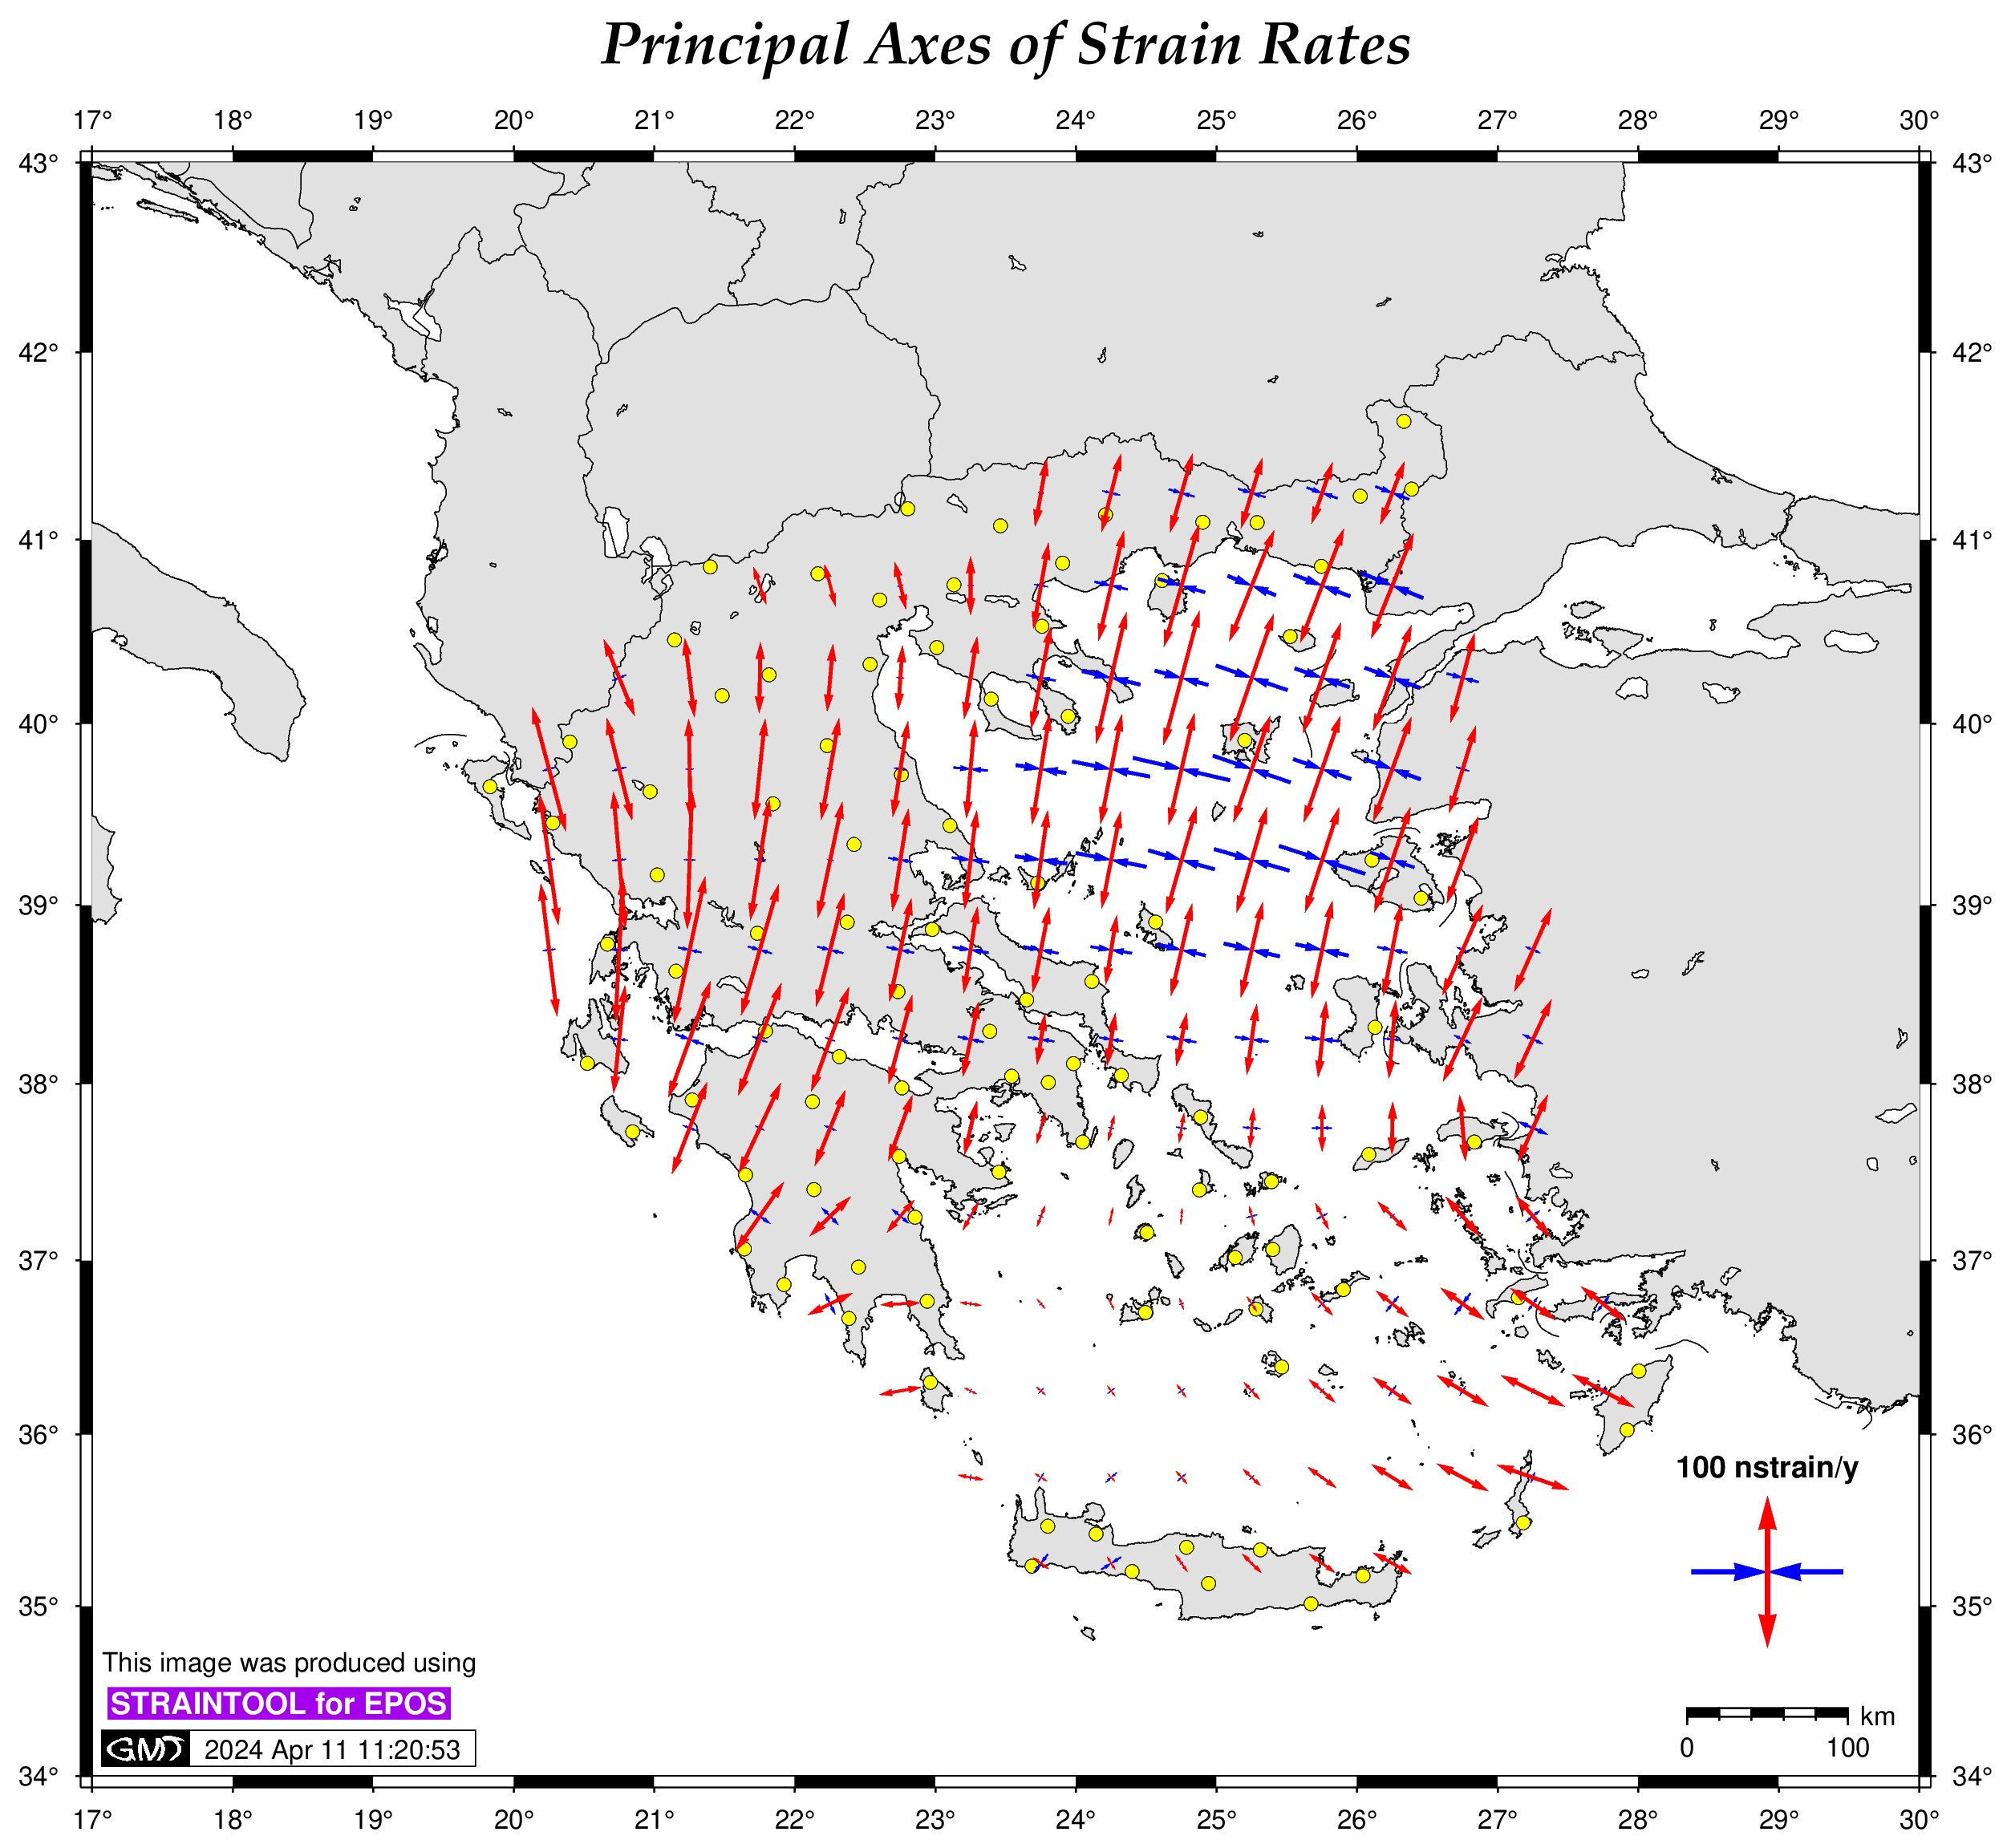
\includegraphics[width=.97\textwidth]{hepos22-output_str.jpg}
\end{minipage}
\begin{minipage}[c]{0.33\linewidth}
  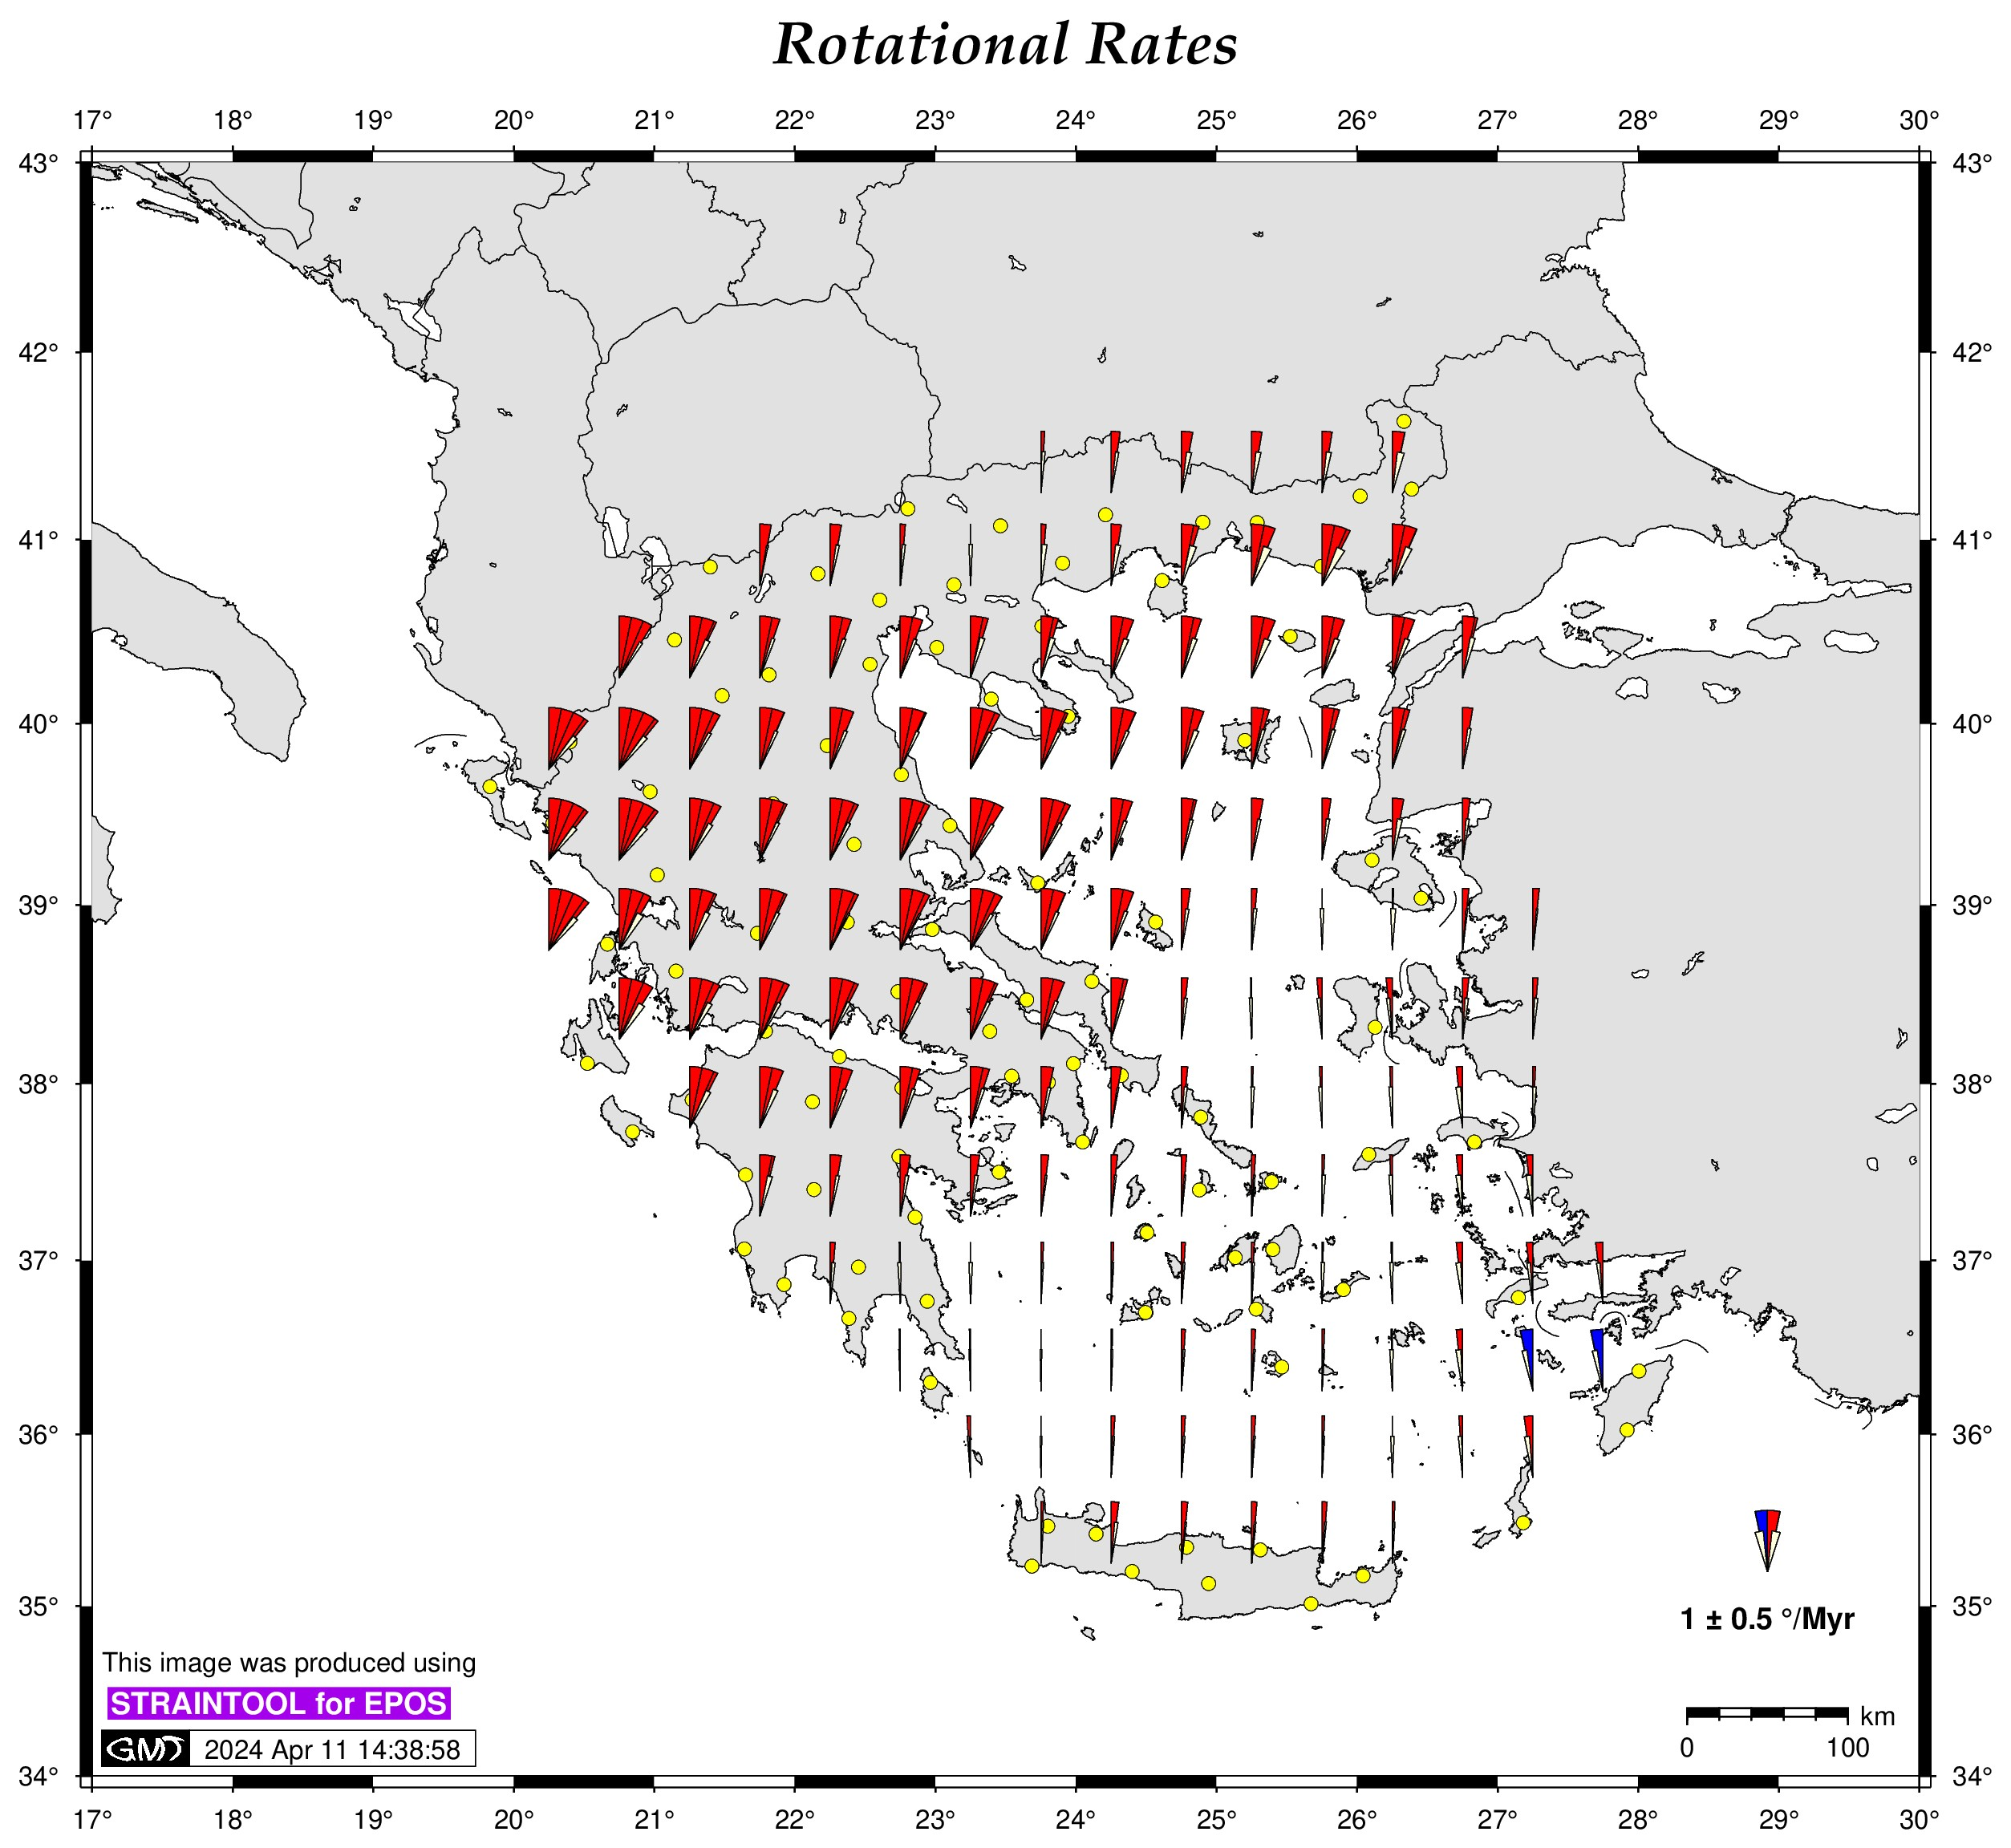
\includegraphics[width=.97\textwidth]{hepos22-output_rot.jpg}
\end{minipage}




%\begin{minipage}[b]{0.60\linewidth}
%Strain-rate results from 302 permanent European GNSS stations are presented in 
%the following maps. The vertical velocity component is ignored in this stage 
%and other sources of deformation (GIA, hydrological, anthropogenic et al.) are 
%not considered in this preliminary interpretation. Different model setups (variable 
%grid-size, distance from cell-center, smoothing parameters etc.) were used for 
%estimation of strain rates. We present results obtained using the following input 
%parameters:
%
%\begin{center}
%\begin{tabular}{ c | c | c | c | c }
%\hline
% grid-size & ltype & dmin & dmax & Wt \\ 
%% \hline
%  0.5$^{\circ} $x0.5$^{\circ} $ & gaussian & 1 km  & 500 km & 6 and 12   \\
%\hline
% \end{tabular}
%\end{center}
%
%Overall, our first results reproduce the gross features of tectonic deformation 
%in Southern Europe, such as NE-SW extension across the Apennines (Italy), NNW-SSE 
%compression across the Alboran Sea (western Mediterranean) and N-S extension in 
%mainland Greece. Large areas of central and Northern Europe show small strain 
%rates (less than 10 ns/yr; 2nd invariant of the tensor).
%
%% \begin{minipage}[t]{0.48\linewidth}
%     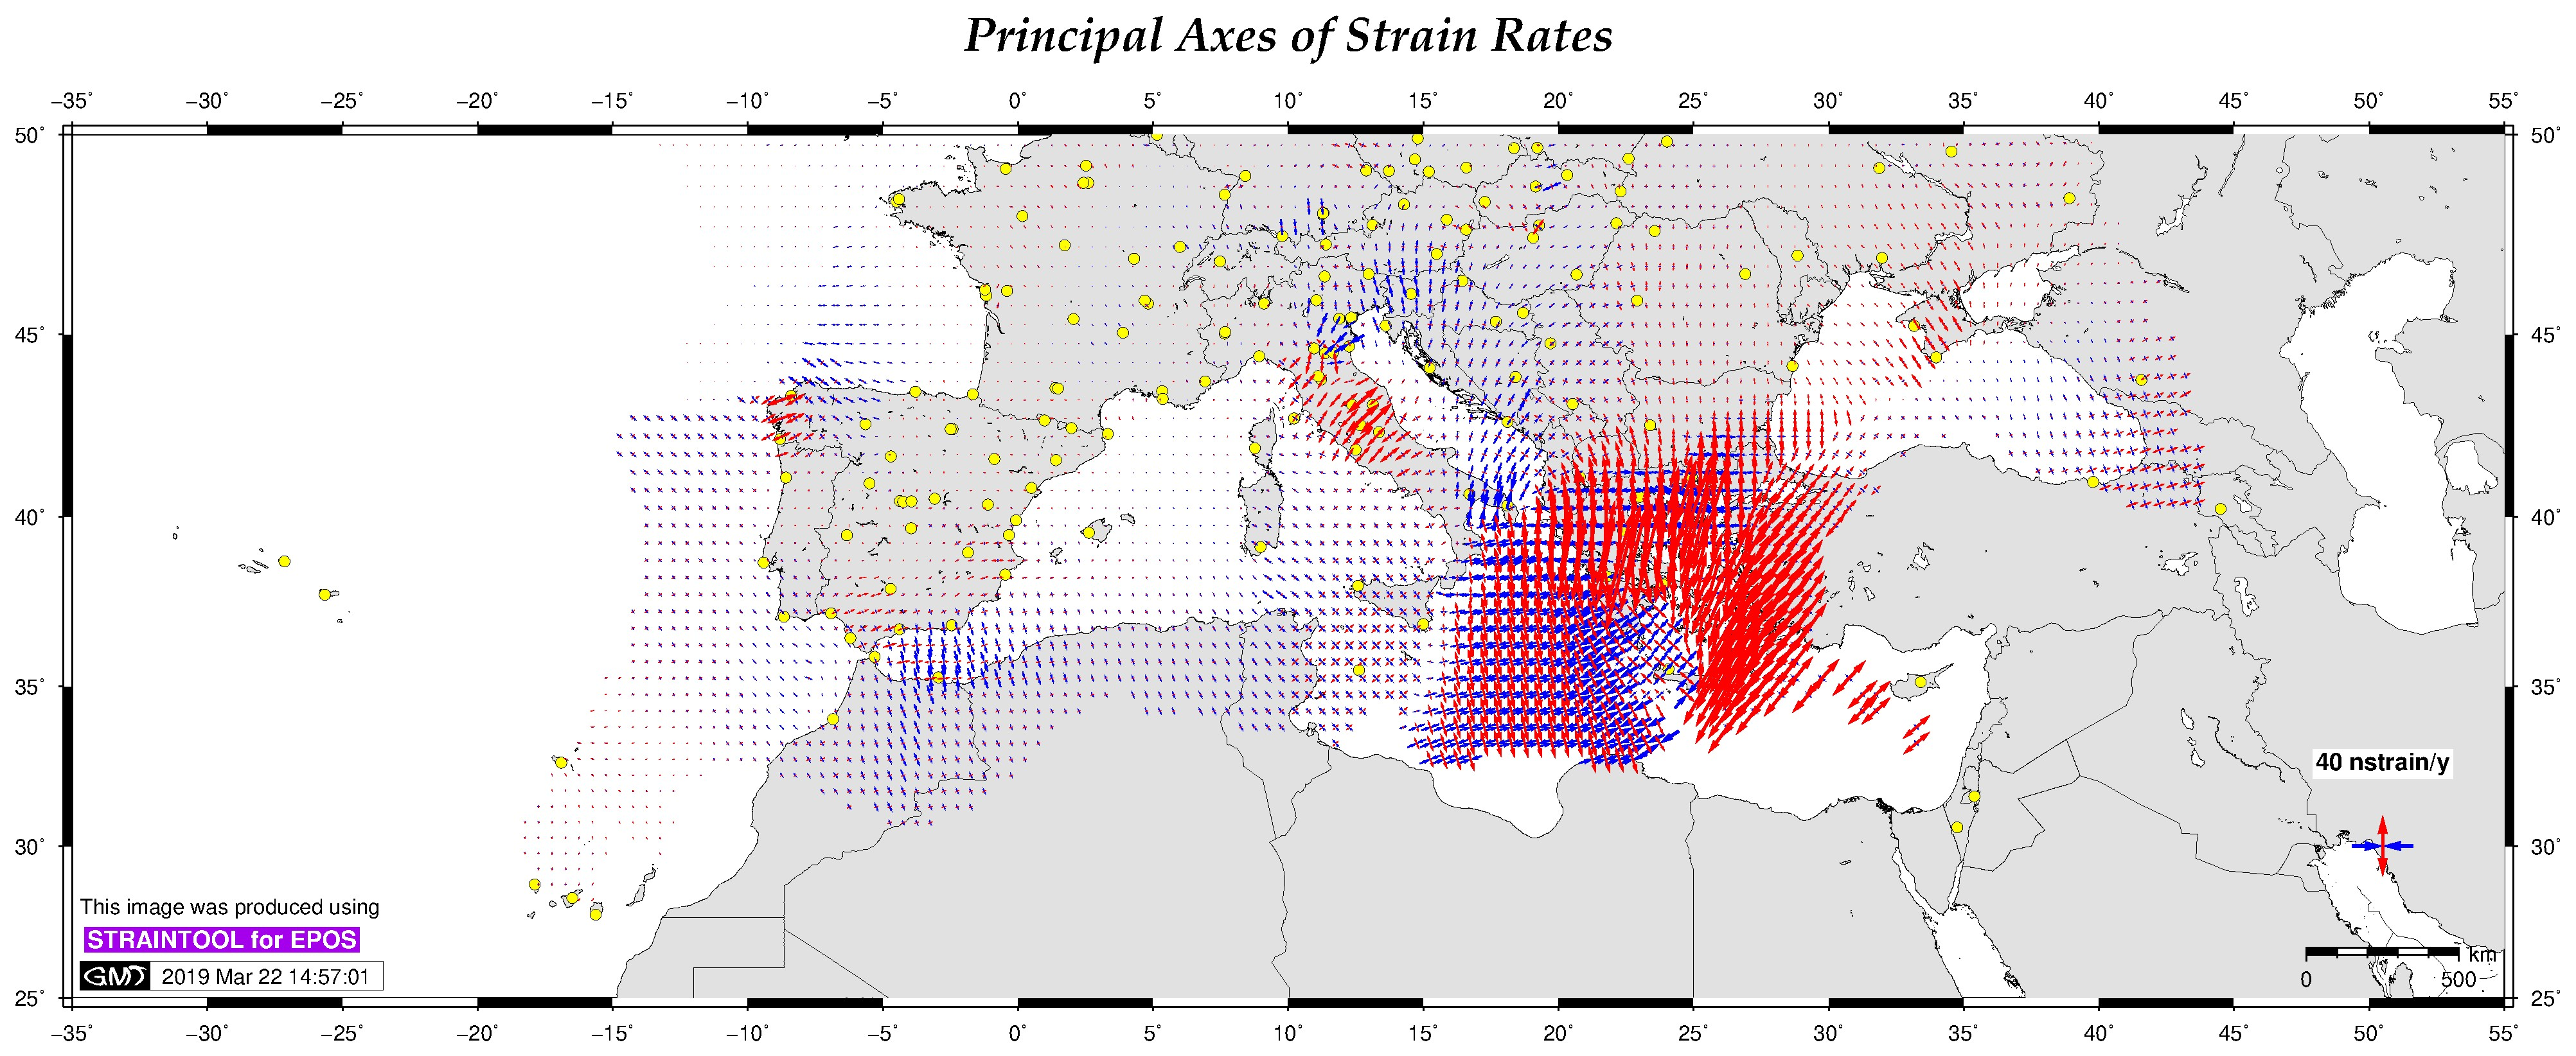
\includegraphics[width=1.07\textwidth]{e14s050506-output_str-S.jpg}
%% \end{minipage}\hfill
%% \begin{minipage}[t]{0.48\linewidth}
%%      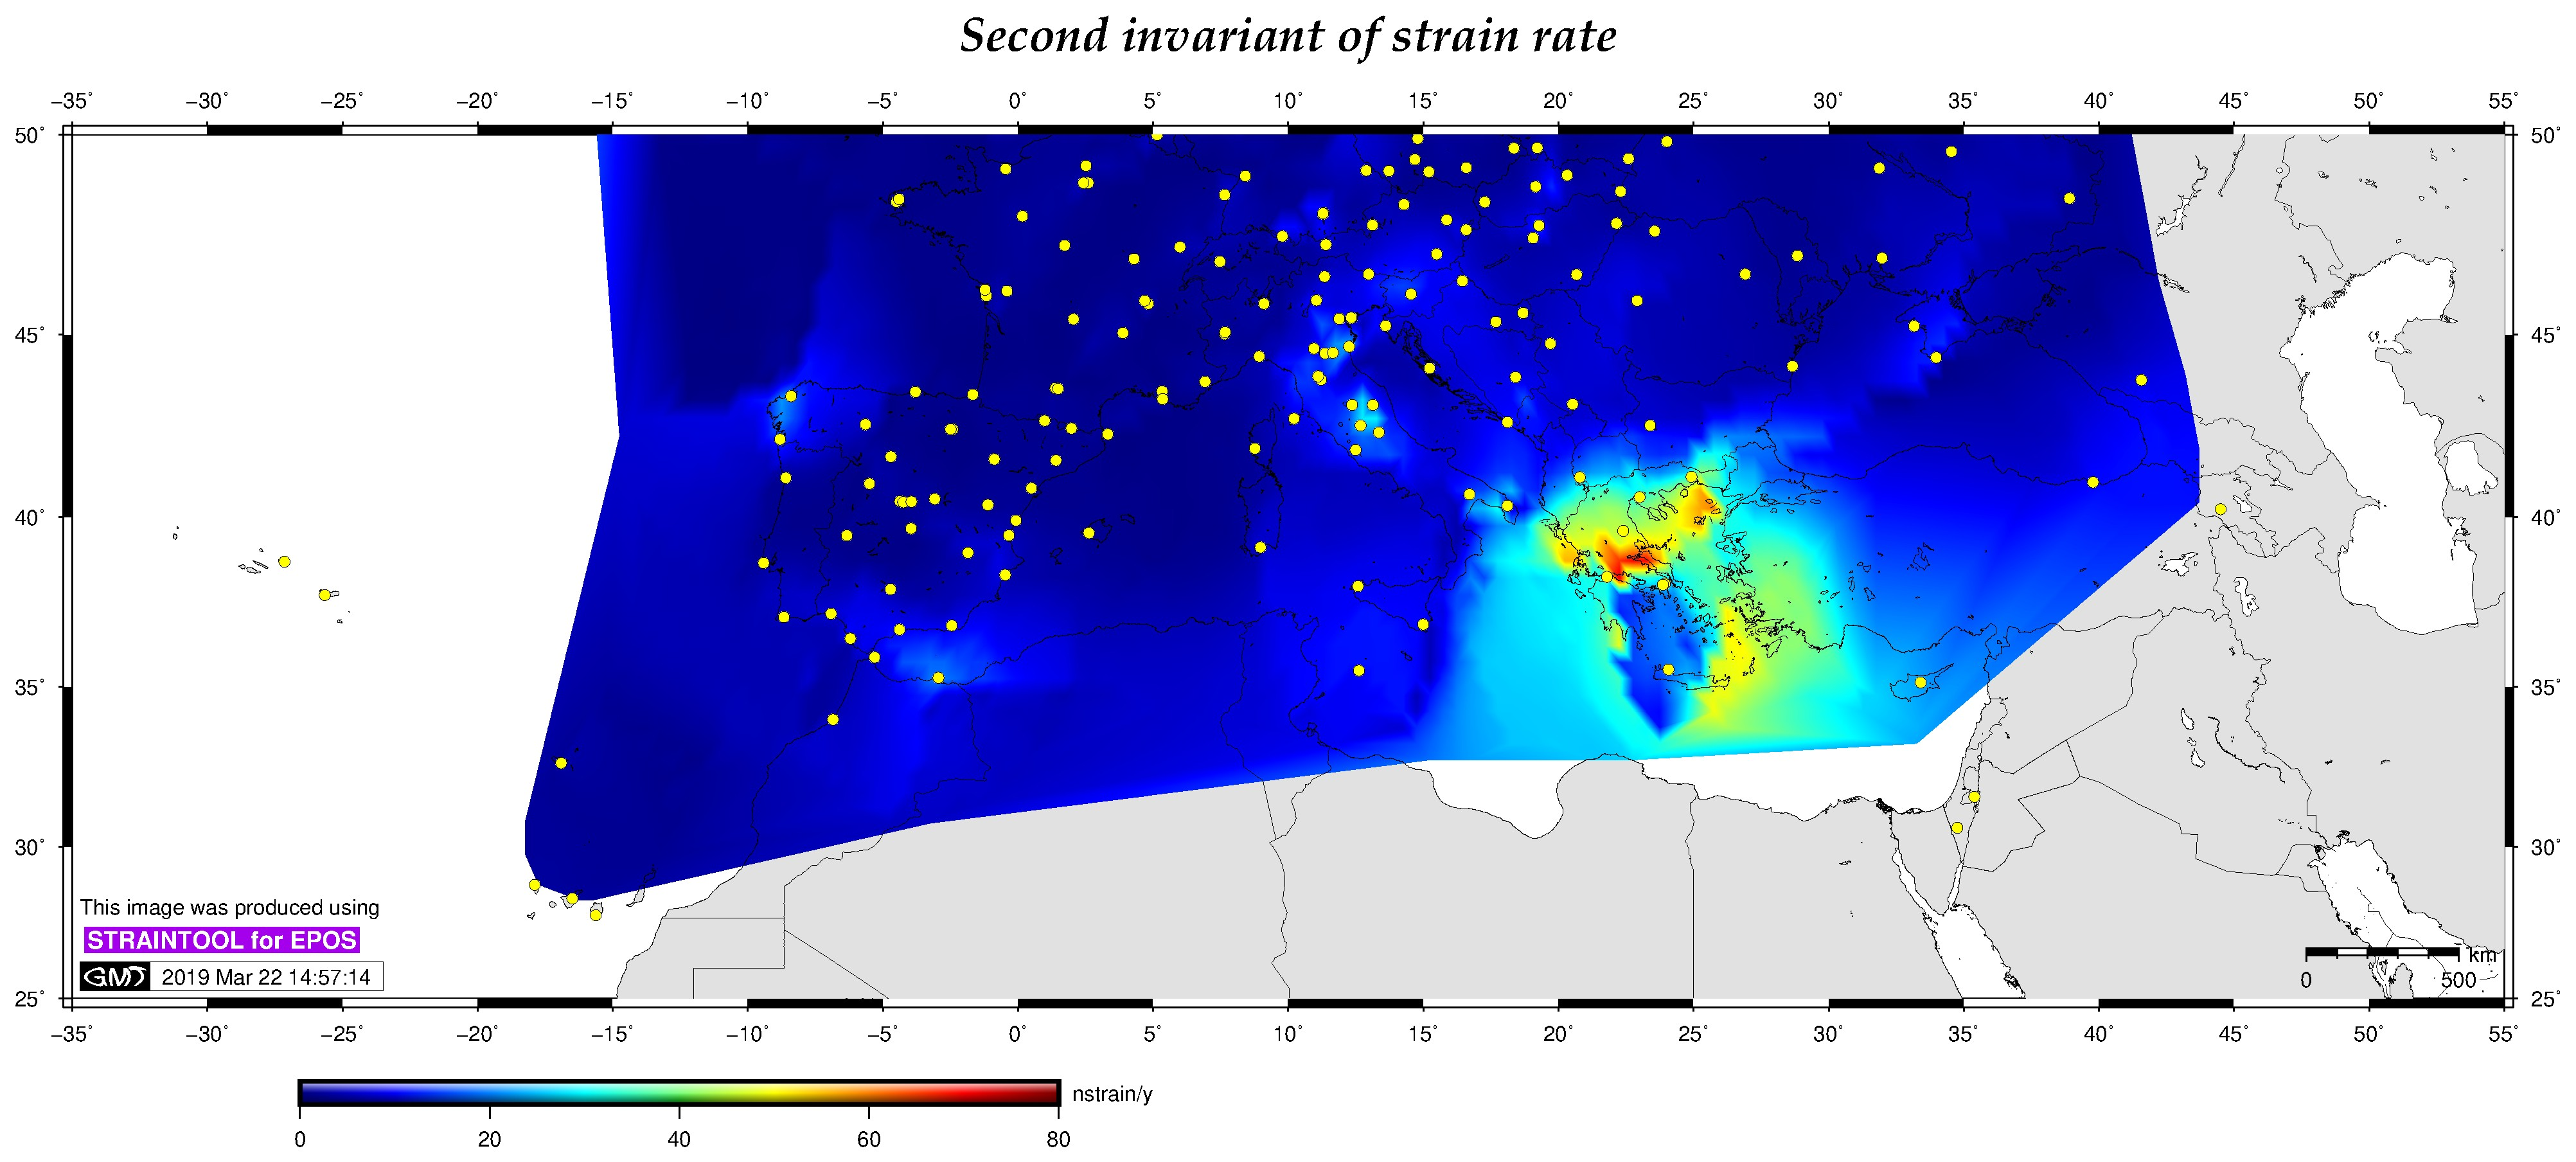
\includegraphics[width=\textwidth]{e14s050506-output_2inv-S.jpg}
%
%% \end{minipage}
%
%\end{minipage}\hfill
%\begin{minipage}[b]{0.36\linewidth}
%     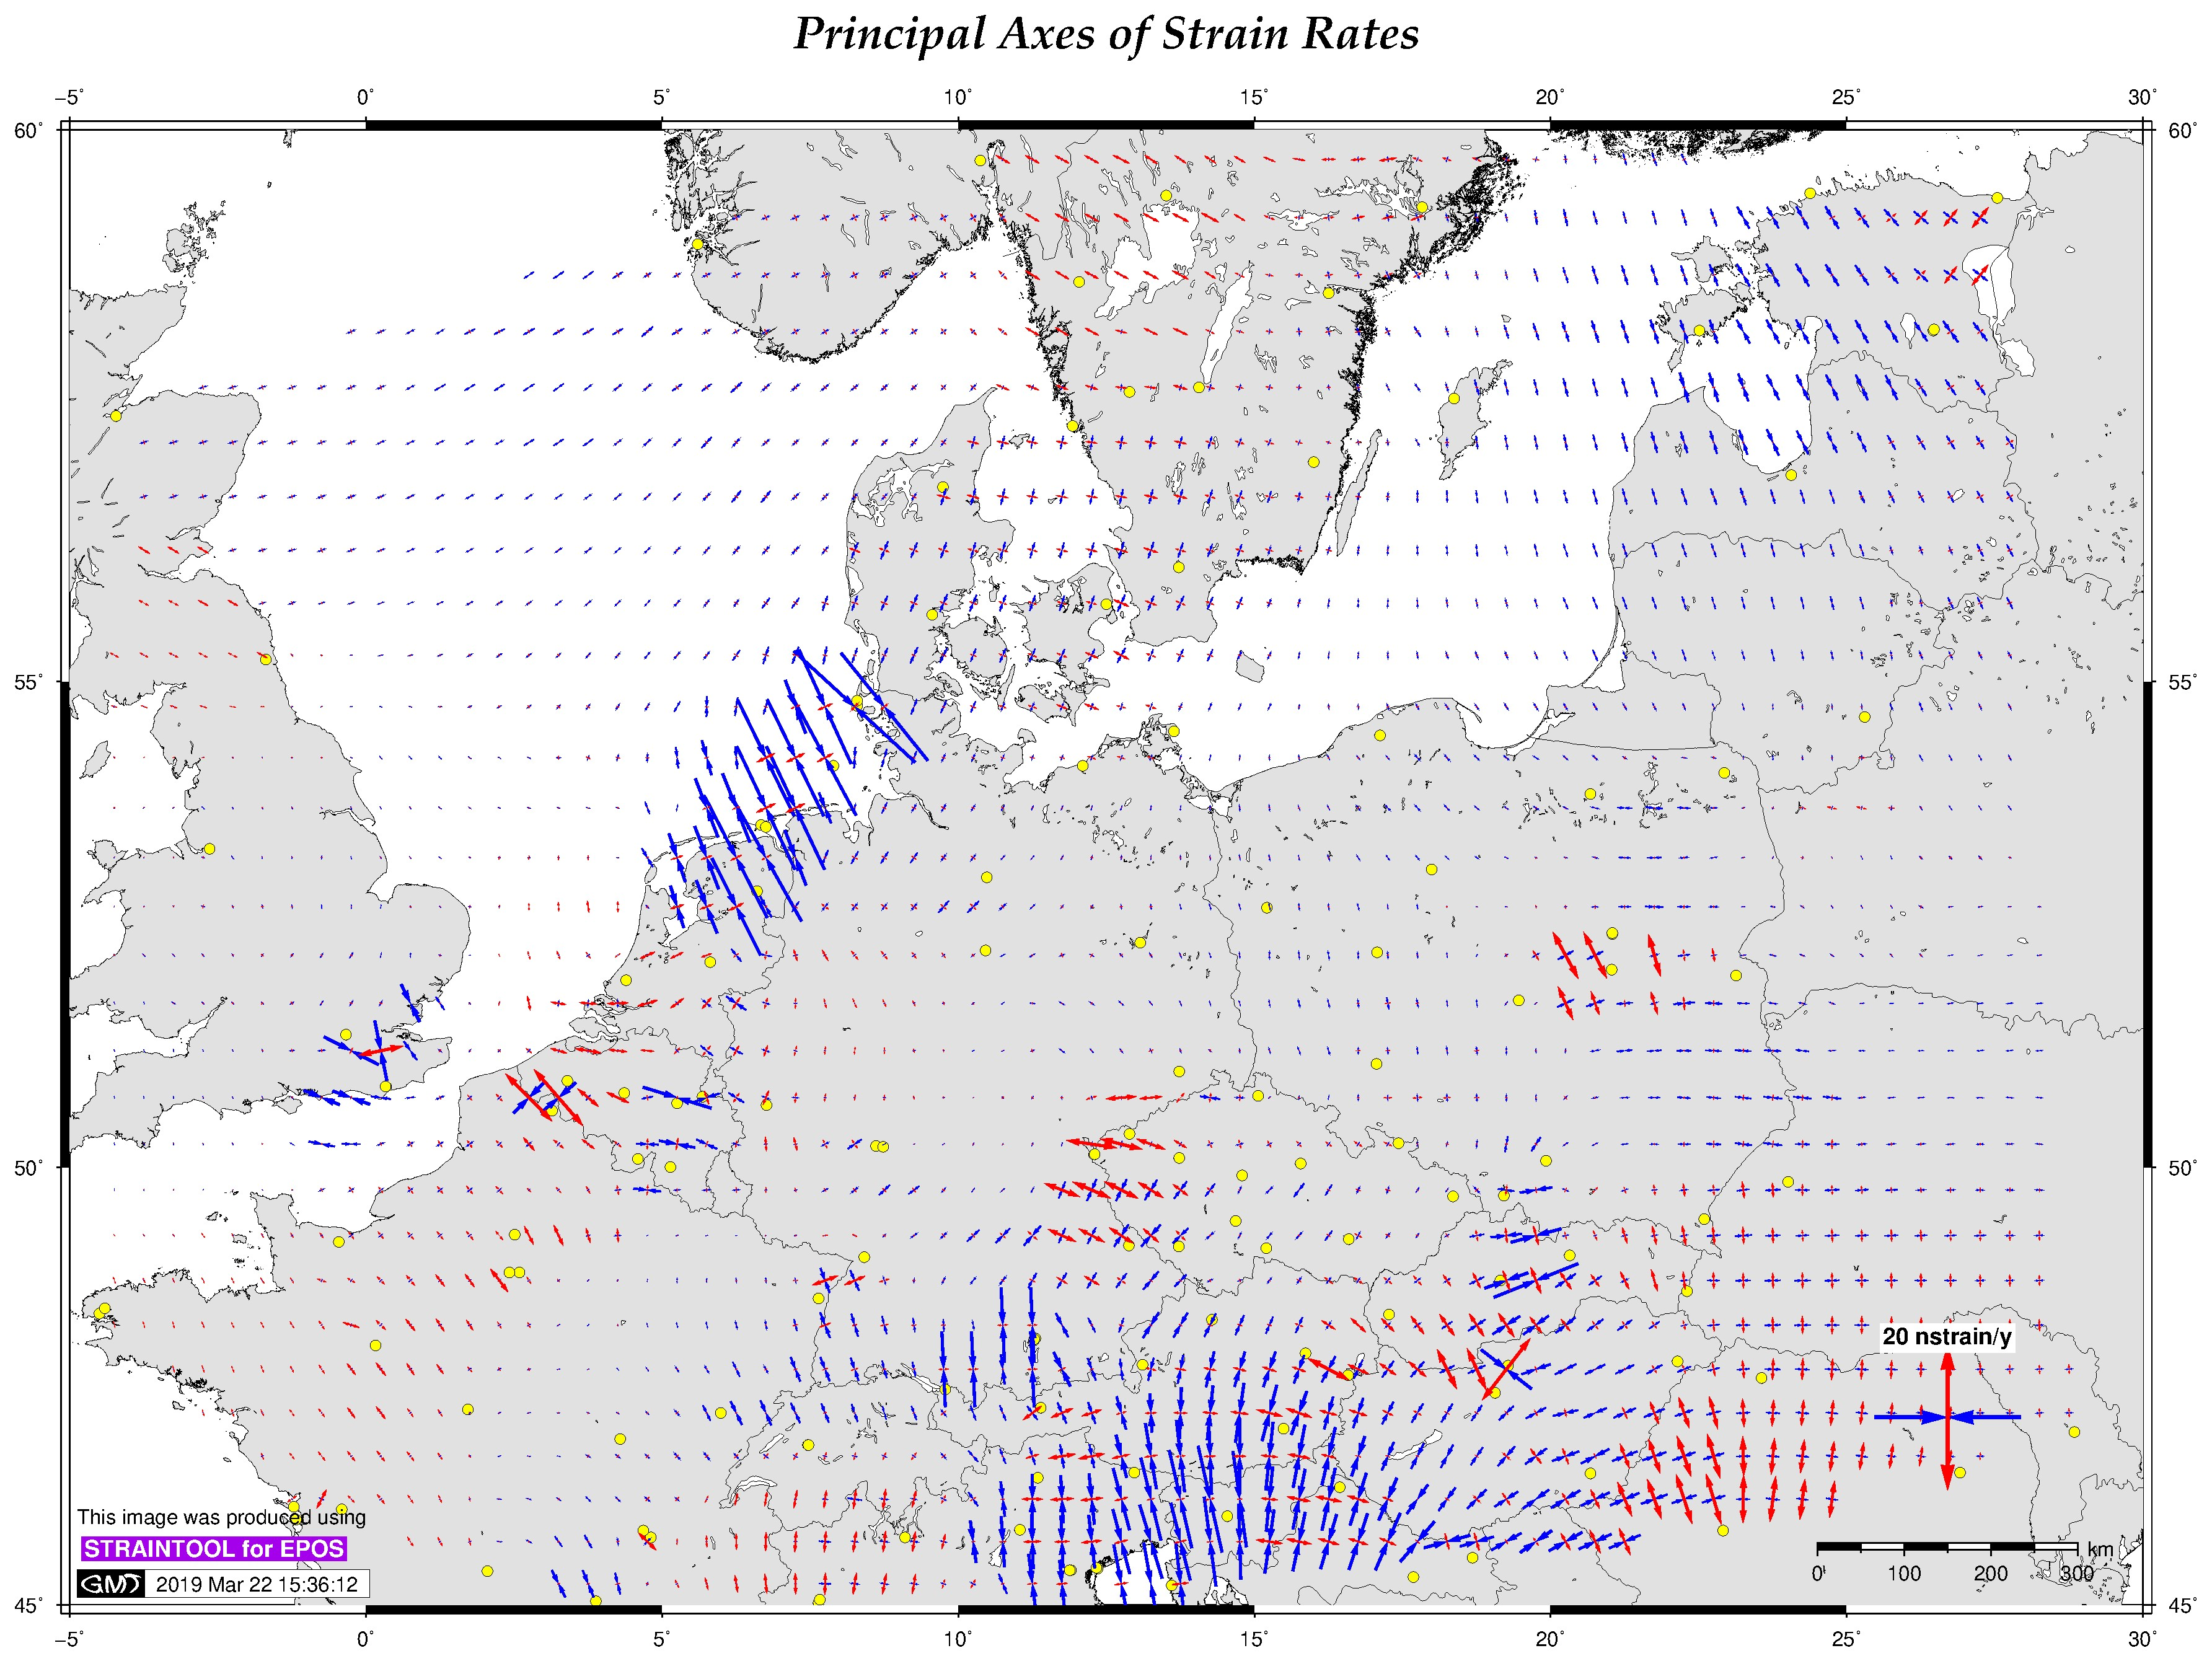
\includegraphics[width=.94\textwidth]{e14np050506e-output_str.jpg}
%     
%%      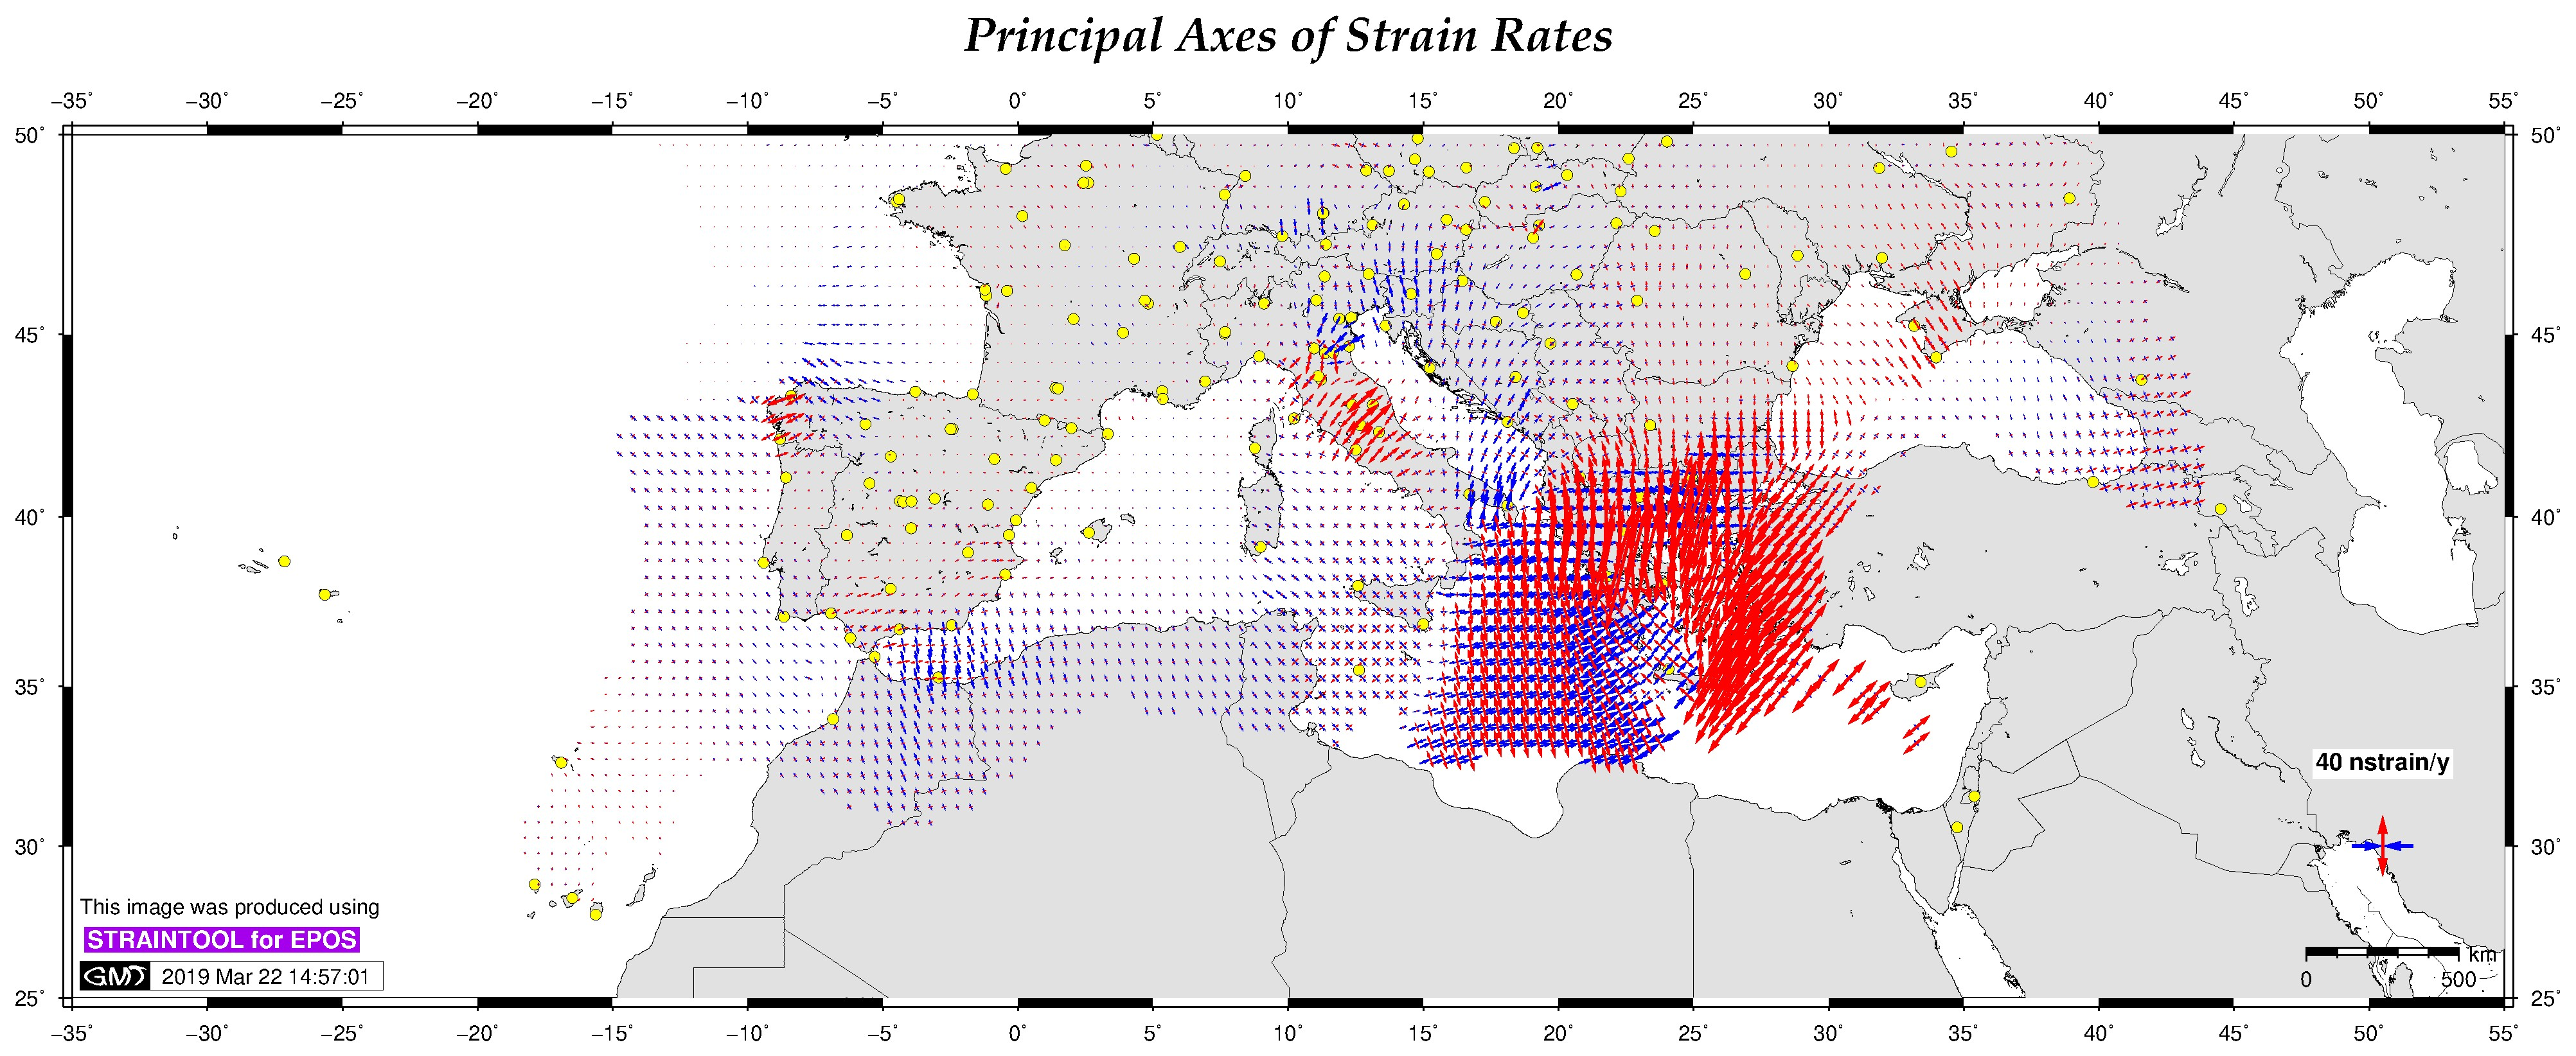
\includegraphics[width=\textwidth]{e14s050506-output_str-S.jpg}
%     
%     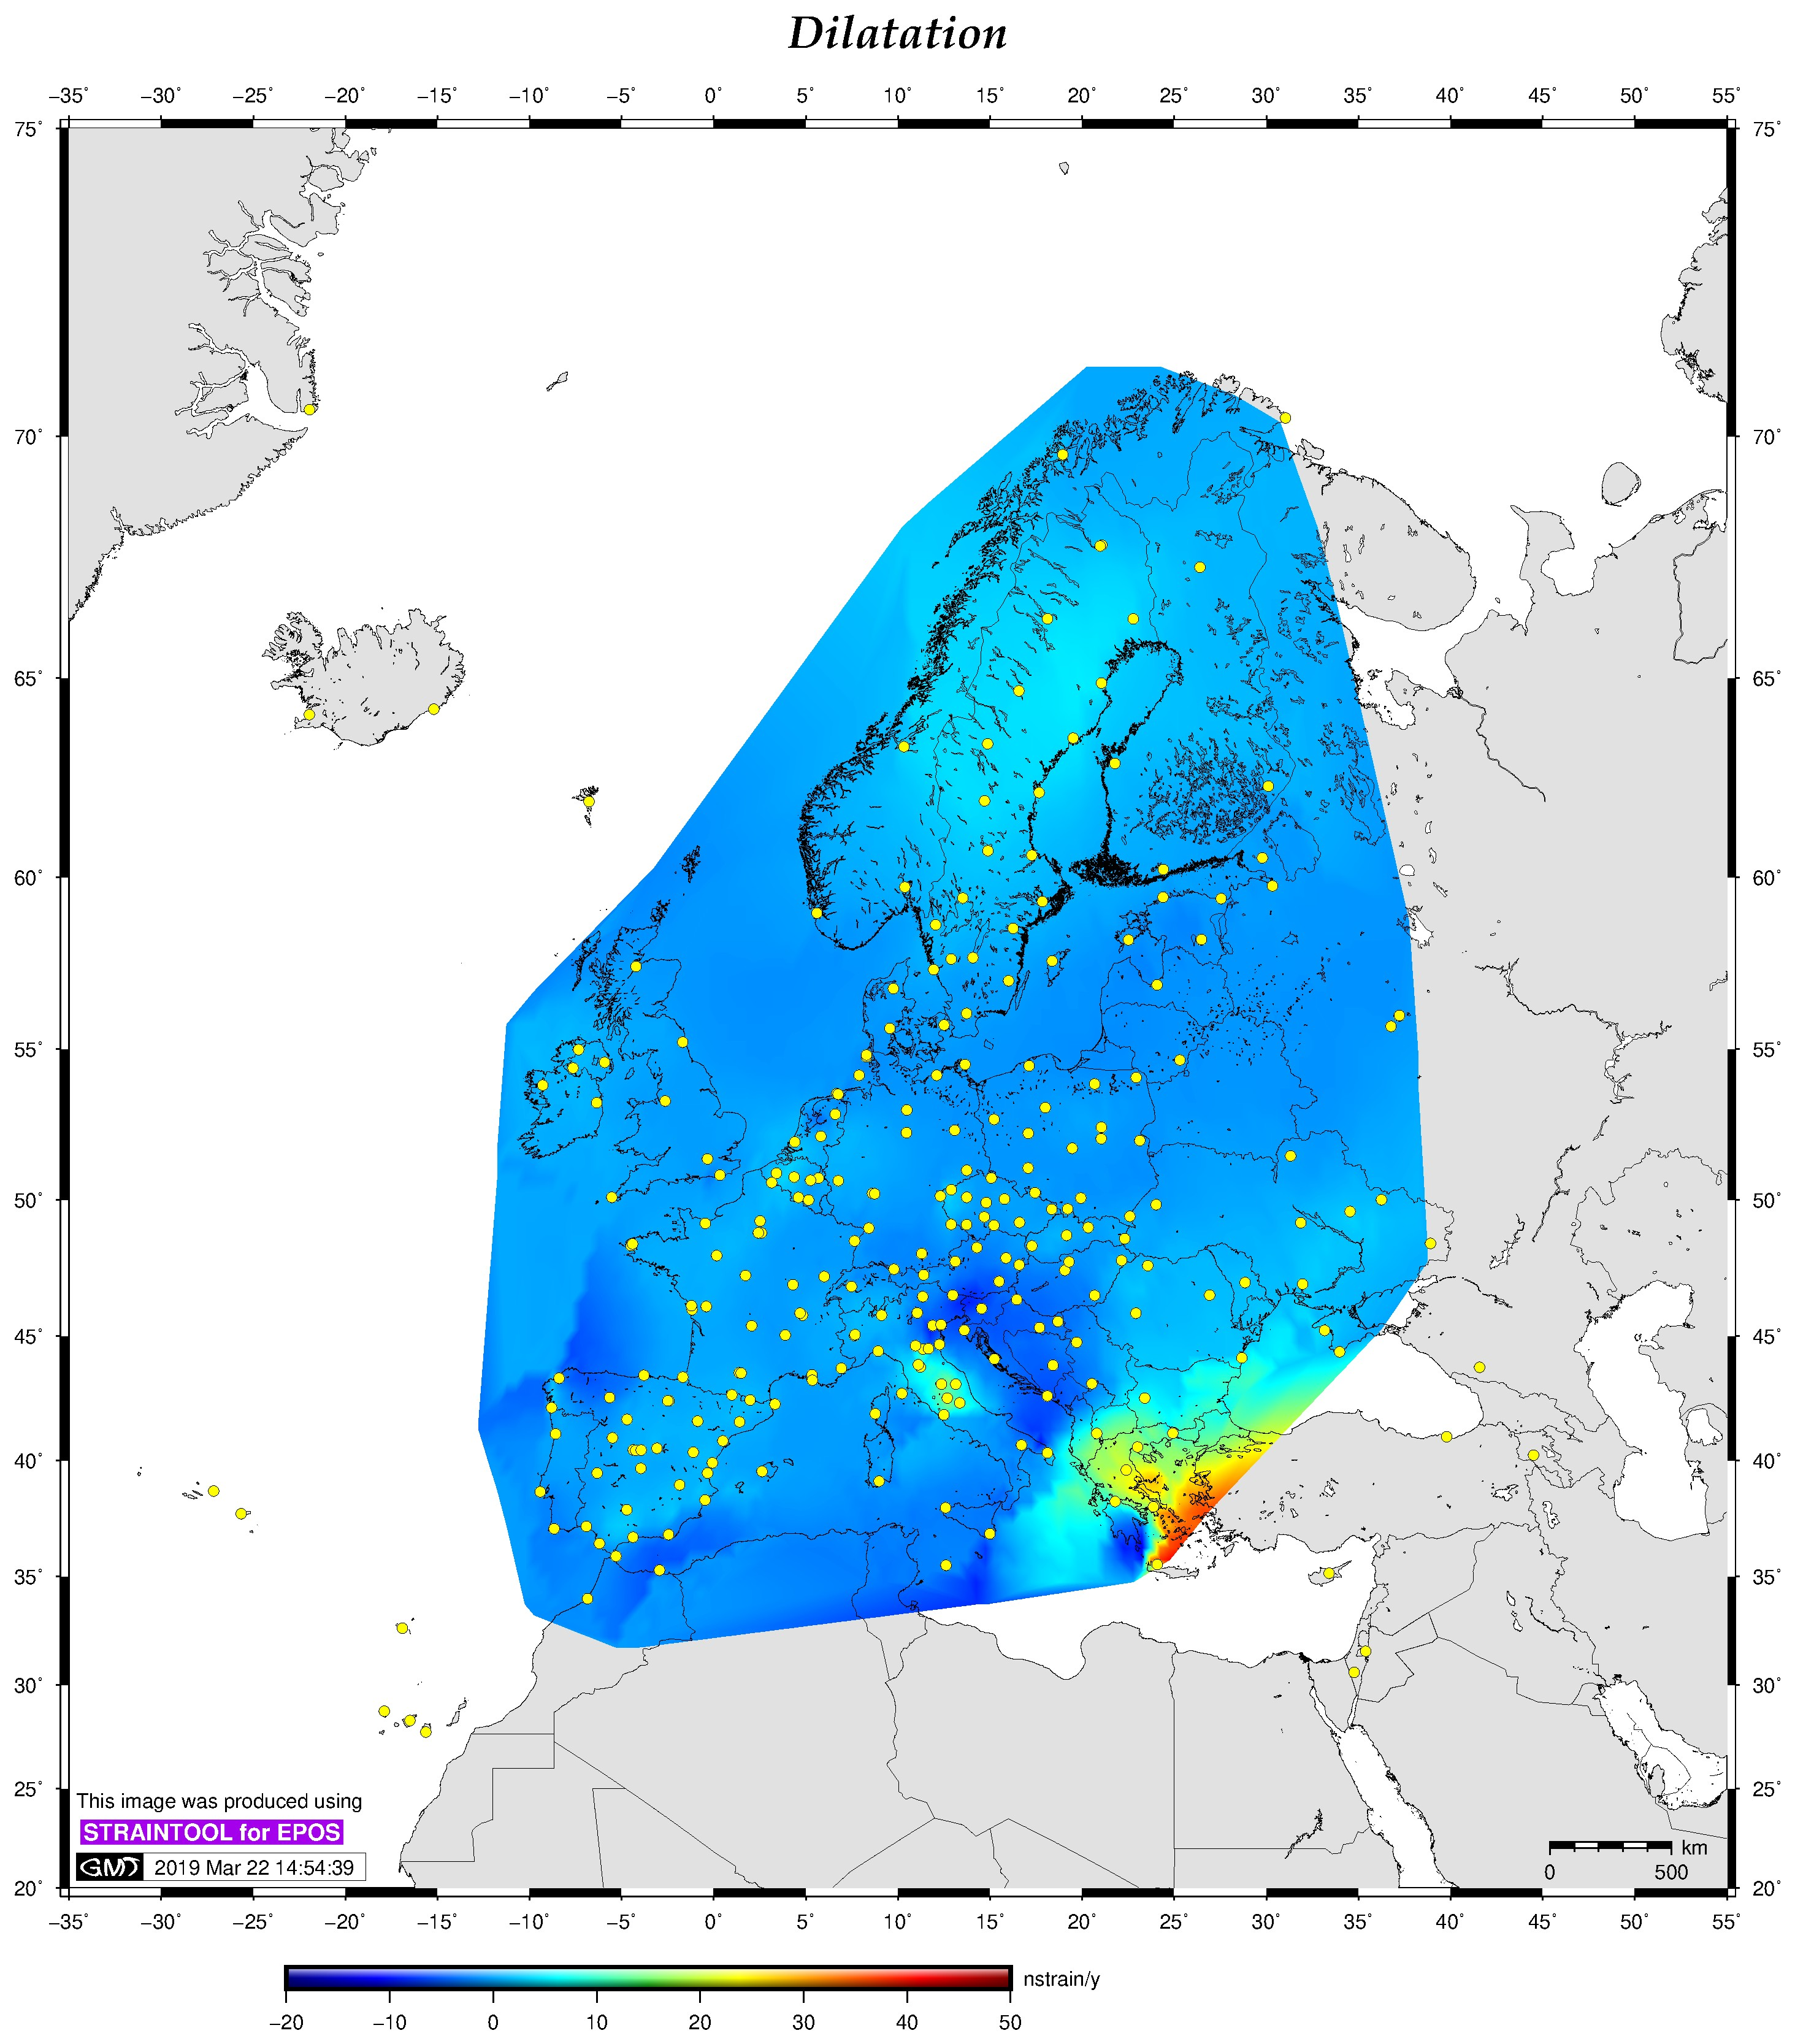
\includegraphics[width=.94\textwidth]{e14s050512-output_dil.jpg}
%\end{minipage}

}

%----------------------------------------------------------------------------------------
%	HEPOS NETWORK
%----------------------------------------------------------------------------------------

\headerbox{HEPOS Network}{name=heposnet,column=0,below=introduction,bottomaligned=resval}{ 
Hellenic Cadastre has since 2007 established a network of 98 continuous GPS sites,spatially
covering the whole country. The network is since maintened by the office, and its products and data used for surveying and supporting national infrastructure.
~\\[1em]
\begin{minipage}[c]{0.49\linewidth}
  \fbox{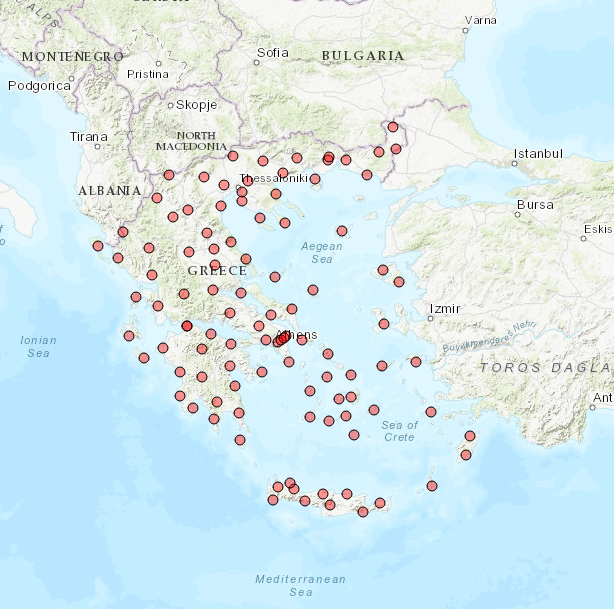
\includegraphics[width=.97\textwidth]{hepos.png}}
\end{minipage}
\begin{minipage}[c]{0.02\linewidth}

\end{minipage}
\begin{minipage}[c]{0.47\linewidth}
  In 2020, Hellenic Cadastre successefully concluded a large-scale upgrade of its network,     introducing a full switch to multi-GNSS. All network sites were equiped with modernized firmware and hardware to support all major GNSS systems (GPS, Glonass, Galileo and Beidou).
\end{minipage}
%In 2020, Hellenic Cadastre successefully concluded a large-scale upgrade of its network, introducing a full switch to multi-GNSS. All network sites were ecquiped with modernized firmware and hardware to support all major GNSS systems (GPS, Glonass, Galileo and Beidou).
~\\[1em]
For this study we analyzed daily RINEX (v.2) files of four individual years, namely 2011, 2015, 2021 and 2022. The data were provided under a special agreement from Hellenic Cadastre to DSO and were selected in a way that could enable the estimation of tectonic behaviour on the one hand, yet require minimum effort and align with the needs and interests of the cadastral office.



%\begin{center}
%  \fbox{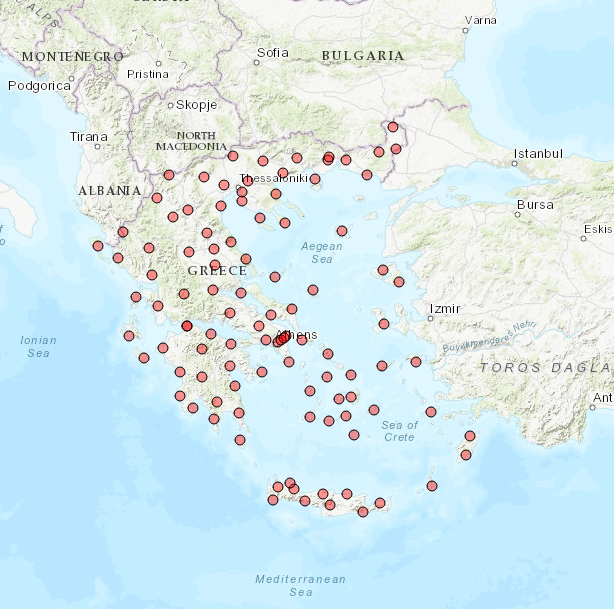
\includegraphics[width=.97\textwidth]{hepos.png}}
%\end{center}
%

}

%----------------------------------------------------------------------------------------
%	STRAIN ALGORITHMS
%----------------------------------------------------------------------------------------

\headerbox{Data Analysis}{name=algorithms,column=1,row=0,bottomaligned=resval}{ 

The data described above were analyzed using the Bernese GNSS Software (v. 5.2) (Dach et al., 2015). Both GPS and GLONASS
observation were used when available (most of 2021 and 2022). IGb14 was used as the frame of reference, using a set of 19 IGS stations for alignment. CODE final products were incorporated in the analysis, consistent with the frame of choice. The key parameter of interest was station coordinates.



%    \footnotesize{The core tool/software is \texttt{Bernese GNSS Software v5.2}.\\
%   %\medskip
%   Integration with
%   \begin{itemize}
%    \setlength\itemsep{.5em}
%     \item \textbf{MySQL} database,
%     \item \textbf{Python} module (product/data downloading, pre-processing, 
%      driving cron jobs, etc)\\
%%      \url{https://github.com/DSOlab/autobern}
%     \item \textbf{Time-series} analysis (integrated in routine processing on regular intervals)
%     \item \textbf{Strain Rates} via StrainTool (on user demand)
%   \end{itemize}}
 \begin{center}
    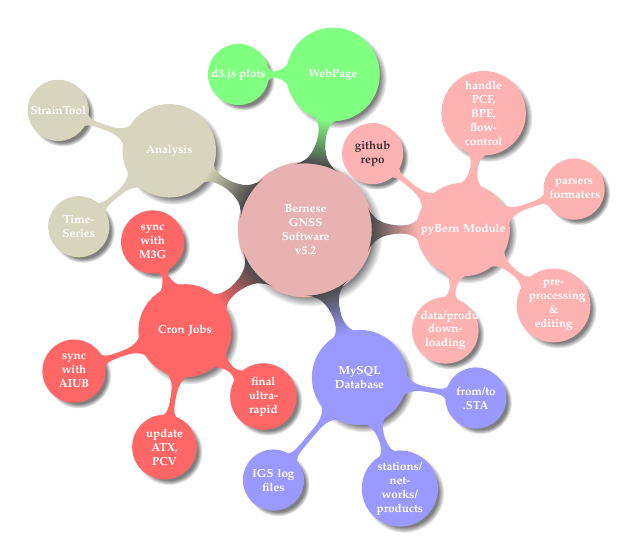
\begin{tikzpicture}[ every annotation/.style = {draw,
                      fill = white, font = \large}]

   \path[mindmap,concept color=black!70,text=white,
     every node/.style={concept,circular drop shadow, scale=.42},
     root/.style = {concept color=black!30!red!30,
font=\normalsize\bfseries,text width=5em},
     level 1 concept/.append style={
       font=\normalsize\bfseries, sibling angle=70,text width=7.7em,
       level distance=20mm,inner sep=0pt},
     level 2 concept/.append style={font=\bfseries,level distance=15mm},
   ]

   node[root] {Bernese GNSS Software v5.2} [clockwise from=0]
     child[concept color=red!30] {
       node {pyBern Module} [clockwise from=140]
       child  [color=black!80] { node {github repo} }
       child  { node {handle PCF, BPE, flow-control} }
       child  { node {parsers\\formaters} }
       child  { node {pre-processing \& editing} }
       child  [level distance=13mm] { node {data/product downloading} }
     }
     child[concept color=blue!40] {
       node[concept] {MySQL Database} [clockwise from=-10]
       child { node[concept] {from/to .STA} }
       child { node[concept] {stations/ networks/ products} }
       child [level distance=17mm] { node[concept] {IGS log files} }
     }
     child[concept color=red!60] {
       node[concept] {Cron Jobs} [clockwise from=-40]
       child [level distance=13mm] { node[concept] {final ultra-rapid} }
       child { node[concept] {update ATX, PCV } }
       child { node[concept] {sync with AIUB} }
       child [level distance=12mm, sibling angle=70] { node[concept]
{sync with M3G} }
     }
     child[concept color=yellow!40!black!30] {
       node[concept] { Analysis } [clockwise from=220]
       child { node[concept] {Time-Series} }
       child [text width=]{ node[concept] {StrainTool} }
     }
     child[concept color=green!50] {
       node[concept] { WebPage } [clockwise from=180]
       child [level distance=12mm, text width=] { node[concept] {d3.js
plots} }
     };
\end{tikzpicture}
 \end{center}
 Processing is consistent with EUREF standards (Guidelines for Analysis Centres).
  \begin{itemize}\setlength\itemsep{.1em}
    \item \texttt{SINEX} with required info/blocks,
    \item Reference frame \texttt{\textcolor{red}{IGb14}},
    \item \texttt{IERS} Conventions 2010,
    \item \texttt{IGS}/\texttt{CODE} products,
    \item ocean loading corrections (\texttt{\textcolor{red}{FES2004}}),
    %\item atmospheric tidal loading corrections,
    \item $3^{\circ}$ elevation cut-off angle; elevation dependent weighting,
    \item \texttt{GMF} and/or \texttt{\textcolor{red}{VMF1}}; \texttt{Chen-Herring} gradient parameter,
    \item amiguities fixed (length-dependent algorithm),
    \item use \texttt{GLONASS} obs (when available)
    \item use \texttt{ATX} files  (\textcolor{red}{epn\_14.atx}) - \textcolor{red}{individual calibrations}
  \end{itemize}


%  $\Rightarrow$ New release Bernese GNSS Software \textcolor{blue}{v5.4}\\[1em]
%  New values on processing options:
%  \begin{itemize}\setlength\itemsep{.5em}
%    \item Reference frame \texttt{\textcolor{blue}{IGS20}}
%    \item Oceans loading corrections (\texttt{\textcolor{blue}{FES2014}})
%    \item \texttt{\textcolor{blue}{VMF3}} for tropospheric modeling
%    \item \texttt{ATX} file: \texttt{\textcolor{blue}{igs20.atx}}
%    \item \textcolor{blue}{Long filename of products} according to new IGS convention
%  \end{itemize}
%  ~\\[.2em]
%  $\Rightarrow$  
%  $\Rightarrow$ Reprocess all available data from late '90s up to now
  
%  \begin{center}
%    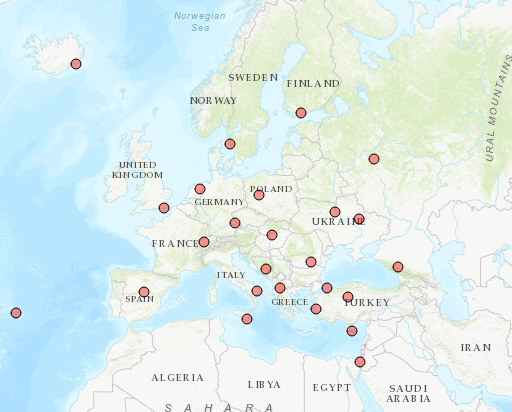
\includegraphics[width=.7\textwidth]{igs.png}
%  \end{center}

 
}

%----------------------------------------------------------------------------------------

\end{poster}

\end{document}
